\chapter{Analysis of processing results}
\label{analysis_processing}
In this chapter the result of the data processing will be evaluated. Starting with the evaluation processing, which clusters the FCD, forms congestion events, finds adjacent incident and exports a list of congestion-incident matched. The second section will elaborate on the results of the correlation processing and use the results for a further analysis of relations.

\section{Evaluation Processing}
\label{analysis_processing_evaluation}
The results of the clustering and matching algorithm where visually reviewed to verify the performance. Thought iterative adjustments of the input parameters the clustering and matching algorithm where calibrated to a sufficient representation level (see final input parameters in \cref{methodology_detection} and \cref{methodology_matching}).

\todo{Add Figures of clustering as proof} 

\section{Correlation Processing}
\label{analysis_processing_correlation}
The resulting datasets created by the evaluation tool (see section \cref{methodology_detection} \cref{methodology_matching} and \cref{methodology_data_processing}) which is tasked with the detection and clustering of jams and search for adjacent incidents, are then processed by the correlation tool (\cref{methodology_correlation_processing}). The correlation tool calculates multiple matrix tables with the correlation effect size, correlation significance and used correction coefficient for all variable combinations. From these tables and interpretation guidelines defined in \cref{correlation_coefficient_types} for each coefficient type, we can deviated the strength of correlation and significance (see \cref{correlation_significance}) for each variable combination. To recap \cref{correlation_coefficient_types}, \cref{tbl:correlation_interpretation_guidelines} shows the guidelines for a weak, moderate and strong correlation effect size of the coefficients $r$,$\eta$,$r_{pq}$,$\tau$ and $V$. The significance is evaluated by an $\alpha$-level of .05.
\begin{table}[ht!]
	\centering
	\begin{tabular}{r|c|c|c}  
		\toprule
		Coefficient & Weak 	& Moderate 	& Strong \\
		\midrule
		$r$ 		& .30	& .50		& .80 \\
		$\eta$ 		& < .06 & .06		& .14 \\
		$r_{pq}$	& < .30	& .30		& .50 \\
		$\tau$ 		& < .30	& .30		& .50 \\
		$V$ 		& < .30	& .30		& .40 \\
		\bottomrule
	\end{tabular}
	\caption{Correlation effect size interpretation for coefficient $r$,$\eta$,$r_{pq}$,$\tau$ and $V$}
	\label{tbl:correlation_interpretation_guidelines}
\end{table}
In the case of correlated and significant variables, it still needs to be determined what the found correlation predicates. This is done via the Post Hoc test, defined in \cref{correlation_posthoc}, which tests for for significance differences between the groups via the pairwise Wilcoxon $T$-test. The rest of this chapter is dedicated to elaborate on this tedious process of testing all groups for significance differences. This involves a enormous number of tables which need to be evaluated and involves repetitions, but is necessary to cover all assumptions and interpretations, referenced later on. For a summary of the significant differences and their interpretations, please forward to \cref{analysis_summary}.

% -------------------------
% -------- BAYSIS ---------
% -------------------------
% Global
% -----------------------------------
% -------- BAYSIS - Matched ---------
% -----------------------------------
\subsection{Congestion - Accidents in general}
\label{analysis_processing_correlation_baysis_matched}
The correlation matrix table for the complete congestion-accident matched dataset (see \cref{table:appendix_correlation_matrix_matched_cramers}) is visual presented in \cref{img:correlation_matrix_matched_cramers} showing the the correlation of each variable combination. When visual analyzing \cref{img:correlation_matrix_matched_cramers} and checking the guidelines for a strong correlation in reference to the applied coefficient (identifiable with \cref{table:appendix_coefficient_matrix_matched}) we get a list of strongly correlated variable combinations (see \cref{tbl:correlation_list_baysis_matched}). Since the focus of the thesis are the correlations between accidents and jams, these are only collected from the bottom-left corner of the matrix, where the congestion and accidents variables intersect. Correlations of the kind congestion - congestion or accident - accident are not considered.
\begin{table}[ht!]
	\centering
	\begin{tabular}{c|l}  
		\toprule
		Category & Strong \\
		\midrule
		Str & TMax, TAvg, SMax, SAvg, TDist, SDist, Cov \\ 
 		Kat & TMax, TAvg, SAvg, TDist \\
 		Typ & TDist, Cov \\
 		%Betei & & \\
 		UArt1 & SAvg, TDist, Cov \\ % + SMax
 		%UArt2 & & \\
 		AUrs1 & SAvg, TDist, SDist, Cov, TLHGV \\ % + SMax
 		%AUrs2 & & \\
 		AufHi & TMax, TAvg, TDist, Cov \\
 		%Alkoh & & \\
 		%Char1 & & \\ % -> Strasse
 		%Char2 & & \\
 		%Bes1 & & \\
 		Lich1 & Cov \\
 		Lich2 & Cov \\ % + Lich2
 		Zust1 & Cov \\ % % -> Strasse
 		%Zust2 & & \\
 		%Fstf & & \\ % -> Strasse
 		WoTag & Cov \\
 		%FeiTag & & \\
		Month & Cov \\ % + TMax. SMAx
		\bottomrule
	\end{tabular}
	\caption{List of incident variables and their strong correlated congestion variable from the congestion-accident matched data}
	\label{tbl:correlation_list_baysis_matched}
\end{table}
Next we need to verify that the correlation is significant and what the correlation predicates. Therefore each correlation will be evaluated with the Post Hoc test, defined in \cref{correlation_posthoc}. \secintroend{baysis}{matched}
\begin{figure}[!ht]
	\centering
	\makebox[\textwidth][c]{%
		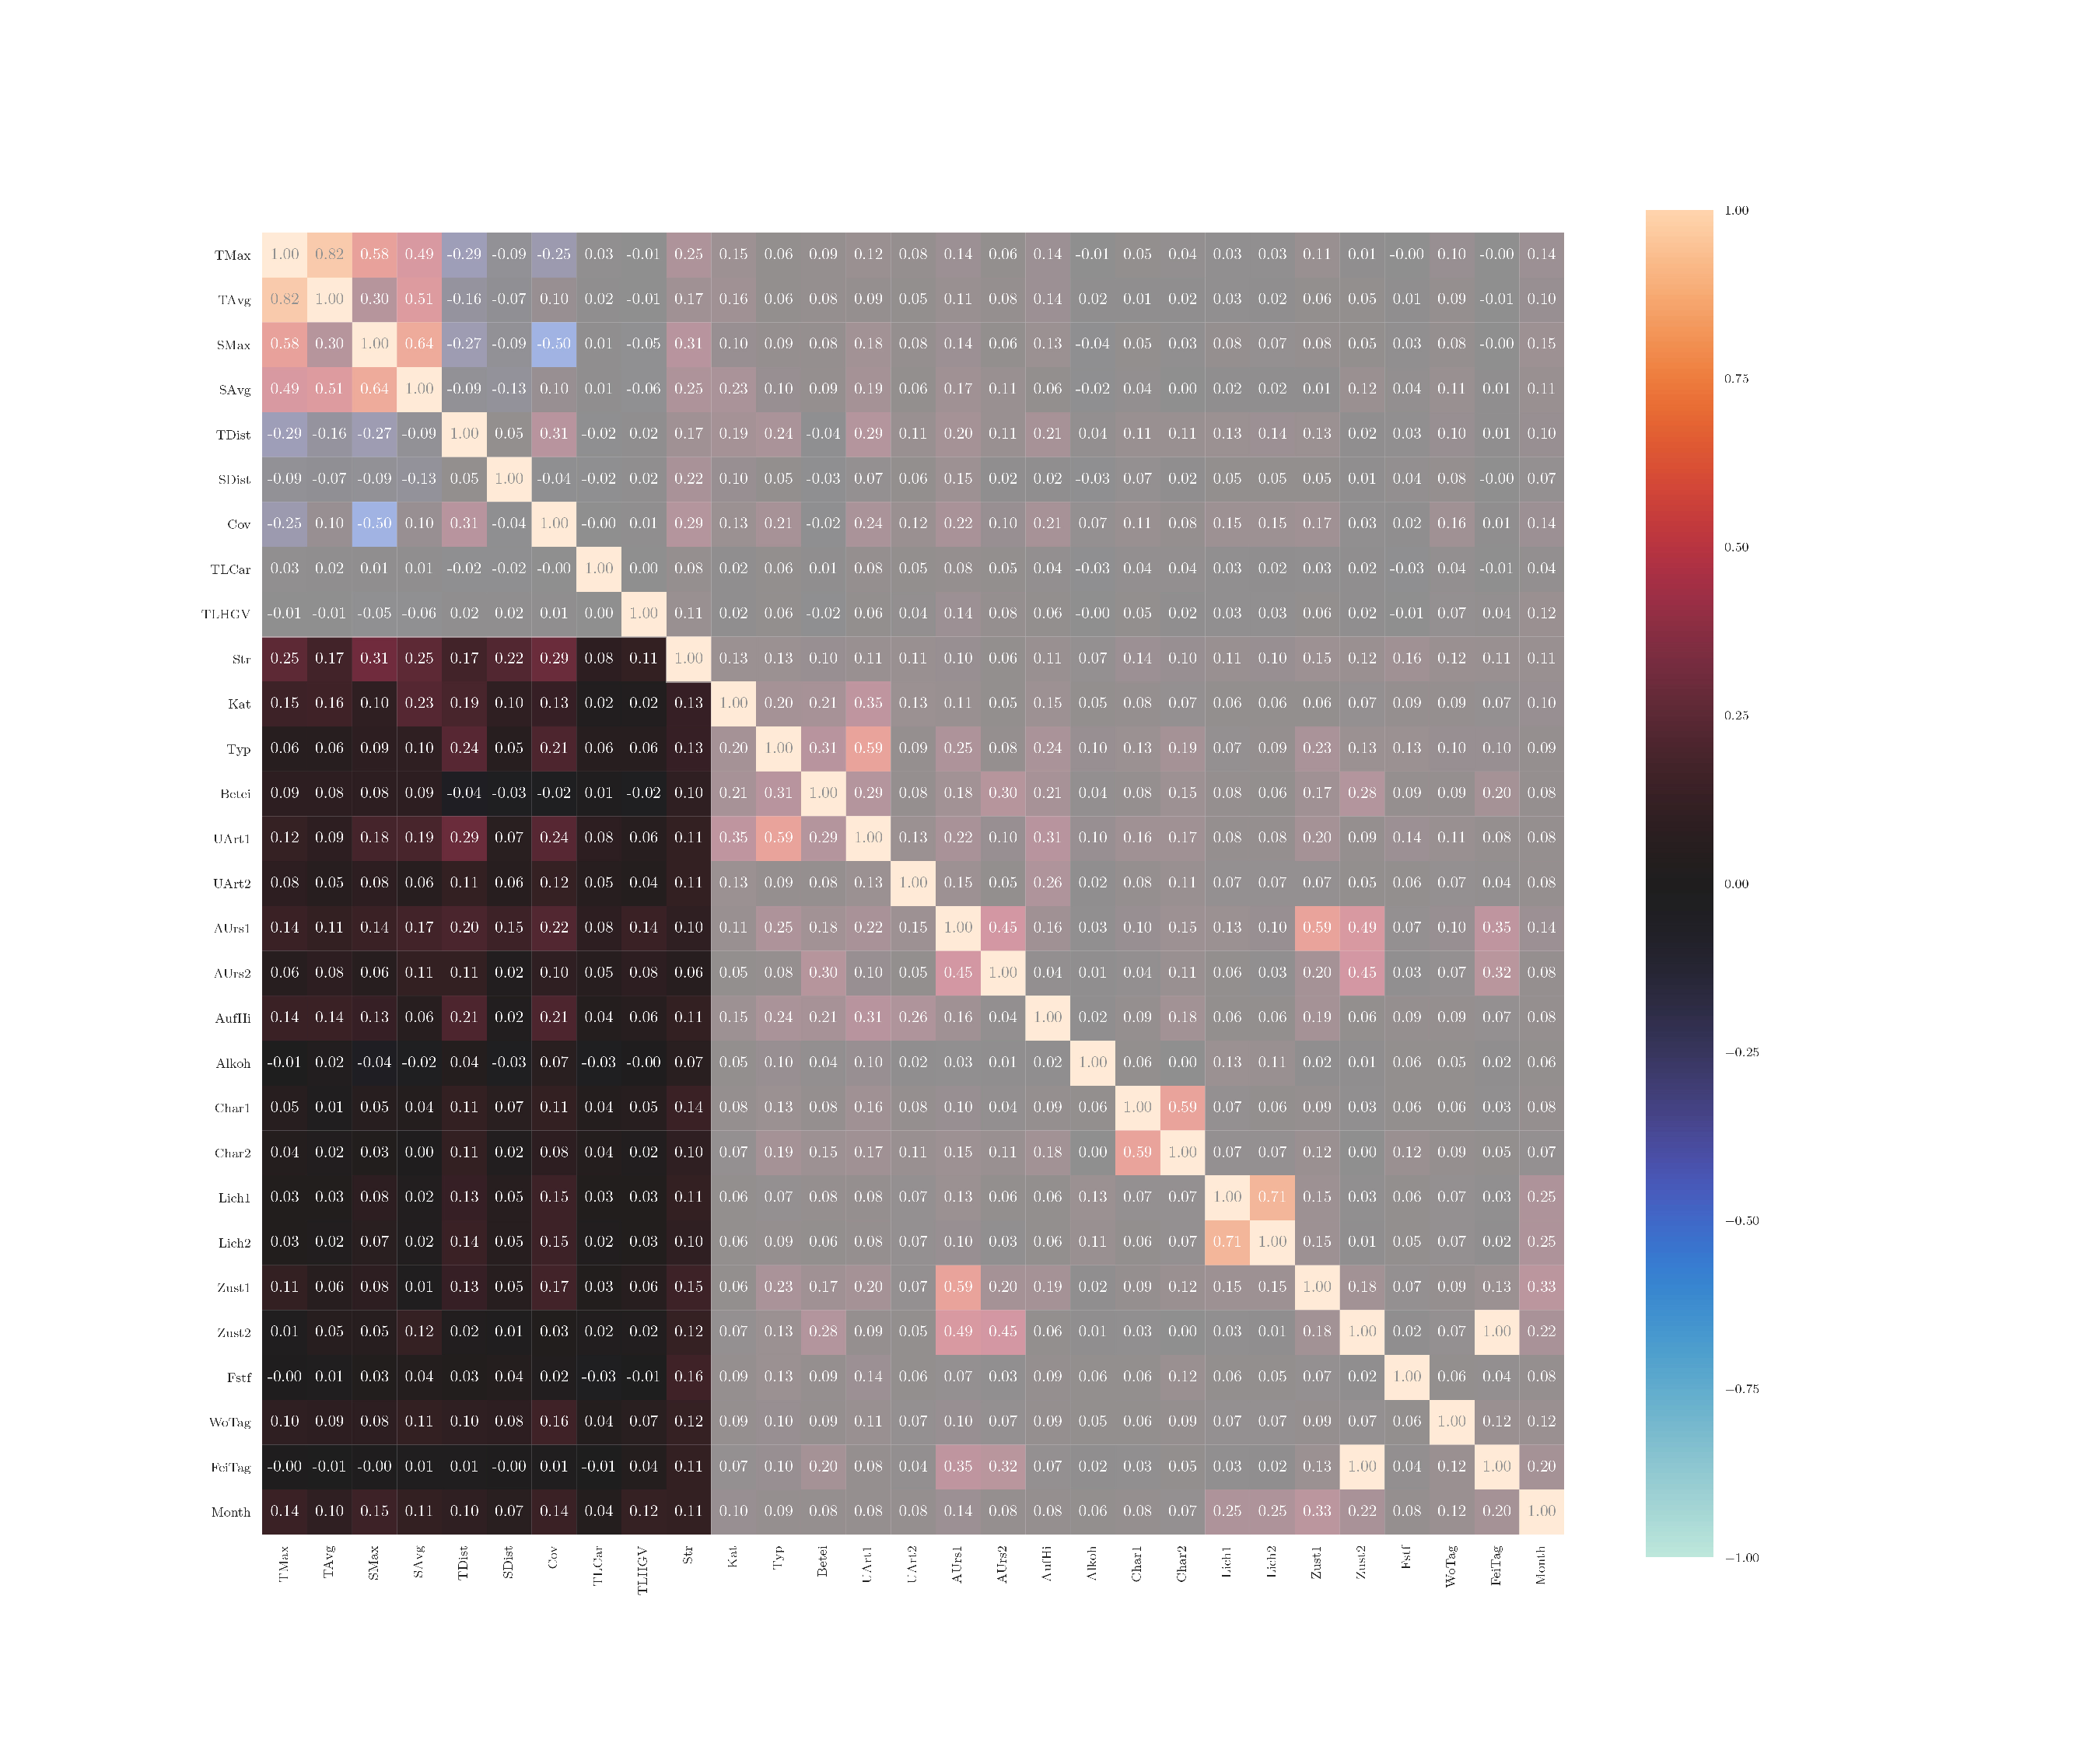
\includegraphics[width=1.4\textwidth, trim=0cm 2.5cm 6cm 3cm]{CorrAnalysis/data/BAYSIS/02_matched/plots/baysis_matched_corr_cramers_edited}%
	}
	\caption{Correlation matrix for congestion-accident matched data calculated with $V$, $\eta$, $\tau$, $r_{pq}$, $r$}
	\label{img:correlation_matrix_matched_cramers}
\end{figure}

% --------------------------
% -------- Strasse ---------
% --------------------------
\centerheading{Street}
\label{ana:baysis_matched_Str}
\varintrosimplewithsam{Str}
\varintronosigmul{Str}{\textit{Str} - \textit{TDist} and \textit{Str} - \textit{SDist}}

% ##############################################
\groupintrosigsig{Str}{TMax}{baysis}{matched}
\begin{table}[ht!]
	\tiny
	\setlength{\tabcolsep}{4pt}
	\centering
	\begin{tabular}{rrrrrrrrrrrrrrrrr}
		\toprule
				& A3 & A6 & A9 & A70 & A96 & A7 & A73 & A99 & A92 & A93 & A94 & A72 & A995 & A95 & A71 & A45 \\ 
		\midrule
		% A6 		& 0.00 &  &  &  &  &  &  &  &  &  &  &  &  &  &  &  \\ 
		A9 		& \red{0.01} & 1.00 &  &  &  &  &  &  &  &  &  &  &  &  &  &  \\ 
		A70 	& \red{0.03} & 1.00 & 1.00 &  &  &  &  &  &  &  &  &  &  &  &  &  \\ 
		A96 	& \red{0.00} & 1.00 & 0.27 & 1.00 &  &  &  &  &  &  &  &  &  &  &  &  \\ 
		A7 		& \red{0.00} & 1.00 & 1.00 & 1.00 & 1.00 &  &  &  &  &  &  &  &  &  &  &  \\ 
		A73 	& \red{0.00} & 1.00 & 0.31 & 1.00 & 1.00 & 1.00 &  &  &  &  &  &  &  &  &  &  \\ 
		% A99 	& 1.00 & 1.00 & 1.00 & 1.00 & 0.50 & 1.00 & 0.59 &  &  &  &  &  &  &  &  &  \\ 
		A92 	& \red{0.00} & 1.00 & 0.16 & 1.00 & 1.00 & 1.00 & 1.00 & 0.22 &  &  &  &  &  &  &  &  \\ 
		% A93 	& 1.00 & 1.00 & 1.00 & 1.00 & 1.00 & 1.00 & 1.00 & 1.00 & 1.00 &  &  &  &  &  &  &  \\ 
		A94 	& \red{0.01} & 1.00 & 1.00 & 1.00 & 1.00 & 1.00 & 1.00 & 1.00 & 1.00 & 1.00 &  &  &  &  &  &  \\ 
		% A72 	& 1.00 & 1.00 & 1.00 & 1.00 & 1.00 & 1.00 & 1.00 & 1.00 & 1.00 & 1.00 & 1.00 &  &  &  &  &  \\ 
		% A995 	& 1.00 & 1.00 & 1.00 & 1.00 & 1.00 & 1.00 & 1.00 & 1.00 & 1.00 & 1.00 & 1.00 & 1.00 &  &  &  &  \\ 
		% A95 	& 1.00 & 1.00 & 1.00 & 1.00 & 1.00 & 1.00 & 1.00 & 1.00 & 1.00 & 1.00 & 1.00 & 1.00 & 1.00 &  &  &  \\ 
		% A71 	& 1.00 & 1.00 & 1.00 & 1.00 & 1.00 & 1.00 & 1.00 & 1.00 & 1.00 & 1.00 & 1.00 & 1.00 & 1.00 & 1.00 &  &  \\ 
		% A45 	& 1.00 & 1.00 & 1.00 & 1.00 & 1.00 & 1.00 & 1.00 & 1.00 & 1.00 & 1.00 & 1.00 & 1.00 & 1.00 & 1.00 & 1.00 &  \\ 
		% A980 	& 1.00 & 1.00 & 1.00 & 1.00 & 1.00 & 1.00 & 1.00 & 1.00 & 1.00 & 1.00 & 1.00 & 1.00 & 1.00 & 1.00 & 1.00 & 1.00 \\ 
		\bottomrule
	\end{tabular}
	\caption{Pairwise Wilcoxon $T$-test for \textit{Street} and \textit{Maximal Temporal Extent}, see \cref{tbl:wilcoxon_baysis_matched_Str_TMax_complete} for complete table}
	\label{tbl:wilcoxon_baysis_matched_Str_TMax}
\end{table}
It shows that the groups A6, A9, A7, A70, A73, A92, A94 and A96 differ significantly from group A3, but there is no distinctive general trend.
% #### START: Table and Plot
\pgfplotstableread[col sep=comma,header=false]{
	A3  , 559 , 225.76 , 210.36 , 156.0 , 9  , 1323 , 1314 
	A6  , 127 , 153.05 , 150.42 , 108.0 , 12 , 864  , 852  
	A9  , 466 , 170.85 , 151.33 , 118.5 , 9  , 1194 , 1185 
	A70 , 31  , 106.55 , 79.42  , 81.0 , 24 , 369  , 345  
	A96 , 155 , 118.32 , 81.05  , 108.0 , 12 , 384  , 372  
	A7  , 130 , 153.37 , 194.10 , 102.0 , 9  , 1341 , 1332 
	A73 , 129 , 125.95 , 135.01 , 93.0 , 12 , 1323 , 1311 
	A99 , 116 , 169.09 , 136.72 , 138.0 , 15 , 681  , 666  
	A92 , 66  , 103.86 , 65.69  , 87.0 , 18 , 354  , 336  
	A93 , 21  , 163.57 , 155.71 , 111.0 , 36 , 588  , 552  
	A94 , 37  , 101.59 , 54.60  , 99.0 , 15 , 249  , 234  
}\data
\pgfplotstablecreatecol[
  create col/expr={\thisrow{1} + \thisrow{2} + \thisrow{3} + \thisrow{4}}
]{sum}{\data}
\begin{figure}[ht!]
	\centering
	\begin{minipage}{0.5\textwidth}
		\tiny
		\setlength{\tabcolsep}{4pt}
		\centering
		\begin{tabular}{c|c|c|c|c|c|c|c}
			\toprule
			Group & $n$ & $\bar{x}$ & $\sigma$ & $\tilde{x}$ & $min$ & $max$ & $\Delta$ \\
			\midrule
			A3  & 559 & 225.76 & 210.36 & 156.0 & 9  & 1323 & 1314 \\ 
			A6  & 127 & 153.05 & 150.42 & 108.0 & 12 & 864  & 852  \\ 
			A9  & 466 & 170.85 & 151.33 & 118.5 & 9  & 1194 & 1185 \\ 
			A70 & 31  & 106.55 & 79.42  & 81.0 & 24 & 369  & 345  \\ 
			A96 & 155 & 118.32 & 81.05  & 108.0 & 12 & 384  & 372  \\ 
			A7  & 130 & 153.37 & 194.10 & 102.0 & 9  & 1341 & 1332 \\ 
			A73 & 129 & 125.95 & 135.01 & 93.0 & 12 & 1323 & 1311 \\ 
			A99 & 116 & 169.09 & 136.72 & 138.0 & 15 & 681  & 666  \\ 
			A92 & 66  & 103.86 & 65.69  & 87.0 & 18 & 354  & 336  \\ 
			A93 & 21  & 163.57 & 155.71 & 111.0 & 36 & 588  & 552  \\ 
			A94 & 37  & 101.59 & 54.60  & 99.0 & 15 & 249  & 234  \\ 
			\bottomrule
			% \bar{x} - sum = , mean = 
			% \sigma - sum = , mean = 
			% \tilde{x}
		\end{tabular}
		\subcaption[second caption.]{Table of all descriptives}\label{tbl:descriptives_baysis_matched_Str_TMax}
	\end{minipage}%
	\begin{minipage}{0.55\textwidth}
		\tiny
		\centering
		\begin{tikzpicture}
			\begin{axis}[
				% Gitterlinien für y-Ticks
				width=\textwidth,
				height=4.7cm,
				xmajorgrids=true,
				ymajorgrids=true,
				xtick=data,
				xmin=0,xmax=10,
				xticklabels from table={\data}{[index]0},
				% zusätzliche Beschriftung an y-Achse
				every extra y tick/.style={
					tick0/.initial=blue,
					tick1/.initial=red,
					yticklabel style={
						color=\pgfkeysvalueof{/pgfplots/tick\ticknum}
					},
				},
				% extra y ticks={201,161},
			]
			\addplot table [absolute series=2] {\data};
			\addplot table [absolute series=3] {\data};
			\addplot table [absolute series=4] {\data};
			\legend{
				$\bar{x}$,$\sigma$,$\tilde{x}$}
			\end{axis}
		 \end{tikzpicture}\vfill
		\subcaption[second caption.]{Plot of descriptives $\bar{x}$, $\sigma$ and $\tilde{x}$}\label{fig:descriptives_baysis_matched_Str_TMax}
	\end{minipage}%
	\caption{Group descriptives of \textit{Street} and \textit{Maximal Temporal Extent}}
	%\vspace{-8mm}
\end{figure}
% #### END: Table and Plot
The descriptives from \cref{tbl:descriptives_baysis_matched_Str_TMax,fig:descriptives_baysis_matched_Str_TMax} show that the mean length of A3 is 27\,\% - 57\,\% higher than the means of A6, A7, A9, A70, A73, A92, and A94. Therefore it can be interpreted that accidents on the A3 are associated with significantly longer (temporal) jams than on the A6, A9, A7, A70, A73, A92, and A94. $\sigma$ and $\tilde{x}$ supports this interpretation with similar features. The descriptives also show three ranked groups of short (A70, A92, A94), medium (A99, A73, A7, A96, A9, A6) and long (A3).

% ##############################################
\groupintrosig{Str}{TAvg}{0.0004}{baysis}{matched}
\begin{table}[ht!]
	\tiny
	\setlength{\tabcolsep}{4pt}
	\centering
	\begin{tabular}{rrrrrrrrrrrrrrrrr}
		\toprule
				& A3 & A6 & A9 & A70 & A96 & A7 & A73 & A99 & A92 & A93 & A94 & A72 & A995 & A95 & A71 & A45 \\ 
		\midrule
		% A6 	 & 0.84 &  &  &  &  &  &  &  &  &  &  &  &  &  &  &  \\ 
		% A9 	 & 0.36 & 1.00 &  &  &  &  &  &  &  &  &  &  &  &  &  &  \\ 
		% A70	 & 1.00 & 1.00 & 1.00 &  &  &  &  &  &  &  &  &  &  &  &  &  \\ 
		% A96  & 0.10 & 1.00 & 1.00 & 1.00 &  &  &  &  &  &  &  &  &  &  &  &  \\ 
		% A7 	 & 1.00 & 1.00 & 1.00 & 1.00 & 1.00 &  &  &  &  &  &  &  &  &  &  &  \\ 
		A73  & \red{0.00} & 1.00 & 0.51 & 1.00 & 1.00 & 1.00 &  &  &  &  &  &  &  &  &  &  \\ 
		A99  & \red{0.02} & 1.00 & 1.00 & 1.00 & 1.00 & 1.00 & 1.00 &  &  &  &  &  &  &  &  &  \\ 
		% A92  & 0.26 & 1.00 & 1.00 & 1.00 & 1.00 & 1.00 & 1.00 & 1.00 &  &  &  &  &  &  &  &  \\ 
		% A93  & 1.00 & 1.00 & 1.00 & 1.00 & 1.00 & 1.00 & 1.00 & 1.00 & 1.00 &  &  &  &  &  &  &  \\ 
		% A94  & 0.28 & 1.00 & 1.00 & 1.00 & 1.00 & 1.00 & 1.00 & 1.00 & 1.00 & 1.00 &  &  &  &  &  &  \\ 
		% A72  & 1.00 & 1.00 & 1.00 & 1.00 & 1.00 & 1.00 & 1.00 & 1.00 & 1.00 & 1.00 & 1.00 &  &  &  &  &  \\ 
		% A995 & 1.00 & 1.00 & 1.00 & 1.00 & 1.00 & 1.00 & 1.00 & 1.00 & 1.00 & 1.00 & 1.00 & 1.00 &  &  &  &  \\ 
		% A95  & 1.00 & 1.00 & 1.00 & 1.00 & 1.00 & 1.00 & 1.00 & 1.00 & 1.00 & 1.00 & 1.00 & 1.00 & 1.00 &  &  &  \\ 
		% A71	 & 1.00 & 1.00 & 1.00 & 1.00 & 1.00 & 1.00 & 1.00 & 1.00 & 1.00 & 1.00 & 1.00 & 1.00 & 1.00 & 1.00 &  &  \\ 
		% A45  & 1.00 & 1.00 & 1.00 & 1.00 & 1.00 & 1.00 & 1.00 & 1.00 & 1.00 & 1.00 & 1.00 & 1.00 & 1.00 & 1.00 & 1.00 &  \\ 
		% A980 & 1.00 & 1.00 & 1.00 & 1.00 & 1.00 & 1.00 & 1.00 & 1.00 & 1.00 & 1.00 & 1.00 & 1.00 & 1.00 & 1.00 & 1.00 & 1.00 \\
		\bottomrule
	\end{tabular}
	\caption{Pairwise Wilcoxon $T$-test for \textit{Street} and \textit{Average Temporal Extent}, see \cref{tbl:wilcoxon_baysis_matched_Str_TAvg_complete} for complete table}
	\label{tbl:wilcoxon_baysis_matched_Str_TAvg}
\end{table}
The table shows that the groups A73 and A99 differ significantly from group A3, but there is no distinctive general trend.
% #### START: Table and Plot
\pgfplotstableread[col sep=comma,header=false]{
	A3  , 559 , 89.66 , 98.94  , 65.00 , 4  , 1260 , 1256 
	A6  , 127 , 69.94 , 65.86  , 56.00 , 3  , 376  , 373  
	A9  , 466 , 72.92 , 64.55  , 54.00 , 4  , 575  , 571  
	A70 , 31  , 50.10 , 23.99  , 49.00 , 10 , 99   , 89   
	A96 , 155 , 61.37 , 44.31  , 52.50 , 5  , 247  , 242  
	A7  , 130 , 86.55 , 146.82 , 59.50 , 6  , 1326 , 1320 
	A73 , 129 , 54.78 , 42.48  , 45.00 , 6  , 274  , 268  
	A99 , 116 , 58.97 , 48.35  , 47.50 , 4  , 295  , 291  
	A92 , 66  , 55.24 , 36.43  , 51.50 , 8  , 235  , 227  
	A93 , 21  , 82.33 , 91.10  , 48.00 , 7  , 343  , 336  
	A94 , 37  , 49.86 , 31.63  , 44.00 , 14 , 145  , 131   
}\data
\pgfplotstablecreatecol[
  create col/expr={\thisrow{1} + \thisrow{2} + \thisrow{3} + \thisrow{4}}
]{sum}{\data}
\begin{figure}[ht!]
	\centering
	\begin{minipage}{0.5\textwidth}
		\tiny
		\setlength{\tabcolsep}{4pt}
		\centering
		\begin{tabular}{c|c|c|c|c|c|c|c}
			\toprule
			Group & $n$ & $\bar{x}$ & $\sigma$ & $\tilde{x}$ & $min$ & $max$ & $\Delta$ \\
			\midrule
			A3  & 559 & 89.66 & 98.94  & 65.00 & 4  & 1260 & 1256 \\ 
			A6  & 127 & 69.94 & 65.86  & 56.00 & 3  & 376  & 373  \\ 
			A9  & 466 & 72.92 & 64.55  & 54.00 & 4  & 575  & 571  \\ 
			A70 & 31  & 50.10 & 23.99  & 49.00 & 10 & 99   & 89   \\ 
			A96 & 155 & 61.37 & 44.31  & 52.50 & 5  & 247  & 242  \\ 
			A7  & 130 & 86.55 & 146.82 & 59.50 & 6  & 1326 & 1320 \\ 
			A73 & 129 & 54.78 & 42.48  & 45.00 & 6  & 274  & 268  \\ 
			A99 & 116 & 58.97 & 48.35  & 47.50 & 4  & 295  & 291  \\ 
			A92 & 66  & 55.24 & 36.43  & 51.50 & 8  & 235  & 227  \\ 
			A93 & 21  & 82.33 & 91.10  & 48.00 & 7  & 343  & 336  \\ 
			A94 & 37  & 49.86 & 31.63  & 44.00 & 14 & 145  & 131  \\ 
			\bottomrule
			% \bar{x} - sum = , mean = 
			% \sigma - sum = , mean = 
			% \tilde{x}
		\end{tabular}
		\subcaption[second caption.]{Table of all descriptives}\label{tbl:descriptives_baysis_matched_Str_TAvg}
	\end{minipage}%
	\begin{minipage}{0.55\textwidth}
		\tiny
		\centering
		\begin{tikzpicture}
			\begin{axis}[
				% Gitterlinien für y-Ticks
				width=\textwidth,
				height=4.7cm,
				xmajorgrids=true,
				ymajorgrids=true,
				xtick=data,
				xmin=0,xmax=10,
				xticklabels from table={\data}{[index]0},
				% zusätzliche Beschriftung an y-Achse
				every extra y tick/.style={
					tick0/.initial=blue,
					tick1/.initial=red,
					yticklabel style={
						color=\pgfkeysvalueof{/pgfplots/tick\ticknum}
					},
				},
				% extra y ticks={201,161},
			]
			\addplot table [absolute series=2] {\data};
			\addplot table [absolute series=3] {\data};
			\addplot table [absolute series=4] {\data};
			\legend{
				$\bar{x}$,$\sigma$,$\tilde{x}$}
			\end{axis}
		 \end{tikzpicture}\vfill
		\subcaption[second caption.]{Plot of descriptives $\bar{x}$, $\sigma$ and $\tilde{x}$}\label{fig:descriptives_baysis_matched_Str_TAvg}
	\end{minipage}%
	\caption{Group descriptives of \textit{Street} and \textit{Average Temporal Extent}}
	%\vspace{-8mm}
\end{figure}
% #### END: Table and Plot
The descriptives from \cref{tbl:descriptives_baysis_matched_Str_TAvg,fig:descriptives_baysis_matched_Str_TAvg} show that the mean value of A3 is about 30\,\% higher than the means of A73 and A96. We can interpret that accidents on the A3 are associated with significantly longer (temporal) jams than on A73 and A96. The descriptives also show general increase of $\bar{x}$ and $\sigma$ around 35\,\% between the roads A94, A92, A73 and A70 to A3, A6, A7 and A9.

% ##############################################
\groupintrosigsig{Str}{TAvg}{baysis}{matched}
\begin{table}[ht!]
	\tiny
	\setlength{\tabcolsep}{4pt}
	\centering
	\begin{tabular}{rrrrrrrrrrrrrrrrr}
		\toprule
				& A3   & A6   & A9   & A70  & A96  & A7   & A73   & A99 & A92 & A93 & A94 & A72 & A995 & A95 & A71 & A45 \\ 
		\midrule
		% A6 		& 0.40 &  &  &  &  &  &  &  &  &  &  &  &  &  &  &  \\ 
		A9 		& \red{0.00} & 1.00 &  &  &  &  &  &  &  &  &  &  &  &  &  &  \\ 
		A70 	& \red{0.00} & 0.83 & 0.54 &  &  &  &  &  &  &  &  &  &  &  &  &  \\ 
		A96 	& \red{0.00} & 1.00 & 0.14 & 1.00 &  &  &  &  &  &  &  &  &  &  &  &  \\ 
		A7 		& \red{0.00} & 1.00 & 1.00 & 1.00 & 1.00 &  &  &  &  &  &  &  &  &  &  &  \\ 
		A73 	& \red{0.00} & \red{0.00} & \red{0.00} & 1.00 & 1.00 & 0.59 &  &  &  &  &  &  &  &  &  &  \\ 
		A99 	& 1.00 & 1.00 & 1.00 & 0.80 & 0.31 & 1.00 & \red{0.00} &  &  &  &  &  &  &  &  &  \\ 
		A92 	& \red{0.00} & \red{0.00} & \red{0.00} & 1.00 & 1.00 & 1.00 & 1.00 & \red{0.00} &  &  &  &  &  &  &  &  \\ 
		A93 	& \red{0.03} & 1.00 & 1.00 & 1.00 & 1.00 & 1.00 & 1.00 & 1.00 & 1.00 &  &  &  &  &  &  &  \\ 
		A94 	& \red{0.00} & 0.11 & \red{0.03} & 1.00 & 1.00 & 1.00 & 1.00 & 0.09 & 1.00 & 1.00 &  &  &  &  &  &  \\ 
		% A72 	& 1.00 & 1.00 & 1.00 & 1.00 & 1.00 & 1.00 & 1.00 & 1.00 & 1.00 & 1.00 & 1.00 &  &  &  &  &  \\ 
		% A995 	& 1.00 & 1.00 & 1.00 & 1.00 & 1.00 & 1.00 & 1.00 & 1.00 & 1.00 & 1.00 & 1.00 & 1.00 &  &  &  &  \\ 
		% A95 	& 1.00 & 1.00 & 1.00 & 1.00 & 1.00 & 1.00 & 1.00 & 1.00 & 1.00 & 1.00 & 1.00 & 1.00 & 1.00 &  &  &  \\ 
		% A71 	& 1.00 & 1.00 & 1.00 & 1.00 & 1.00 & 1.00 & 1.00 & 1.00 & 1.00 & 1.00 & 1.00 & 1.00 & 1.00 & 1.00 &  &  \\ 
		% A45 	& 1.00 & 1.00 & 1.00 & 1.00 & 1.00 & 1.00 & 1.00 & 1.00 & 1.00 & 1.00 & 1.00 & 1.00 & 1.00 & 1.00 & 1.00 &  \\ 
		% A980 	& 1.00 & 1.00 & 1.00 & 1.00 & 1.00 & 1.00 & 1.00 & 1.00 & 1.00 & 1.00 & 1.00 & 1.00 & 1.00 & 1.00 & 1.00 & 1.00 \\ 
		\bottomrule
	\end{tabular}
	\caption{Pairwise Wilcoxon $T$-test for \textit{Street} and \textit{Maximal Spatial Extent}, see \cref{tbl:wilcoxon_baysis_matched_Str_SMax_complete} for complete table}
	\label{tbl:wilcoxon_baysis_matched_Str_SMax}
\end{table}
It shows, that the groups A7, A9, A70, A73, A92, A94 and A96 differ from group A3. The groups A73 and A92 further differ from group A6 and A9. The group A99 differs from group A73 and group A92 differs from A99, but there is no distinctive general trend.
% #### START: Table and Plot
\pgfplotstableread[col sep=comma,header=false]{
	A3  , 559 , 13874.96 , 10064.51 , 11014.00 , 1084 , 46328 , 45244 
	A6  , 127 , 11067.98 , 8428.07  , 8634.00  , 965  , 43156 , 42191 
	A9  , 466 , 10680.48 , 7724.45  , 8977.50  , 832  , 49765 , 48933 
	A70 , 31  , 6676.39  , 3640.24  , 6136.00  , 1841 , 13058 , 11217 
	A96 , 155 , 8551.75  , 6431.18  , 6238.00  , 971  , 27965 , 26994 
	A7  , 130 , 9018.27  , 7293.14  , 7051.50  , 1108 , 43244 , 42136 
	A73 , 129 , 6502.88  , 5033.20  , 5327.00  , 1036 , 33764 , 32728 
	A99 , 116 , 13244.02 , 11313.27 , 9439.50  , 1280 , 48278 , 46998 
	A92 , 66  , 6186.80  , 4000.10  , 4936.50  , 1176 , 23291 , 22115 
	A93 , 21  , 6765.00  , 4403.32  , 5323.00  , 1244 , 16922 , 15678 
	A94 , 37  , 6220.38  , 3984.46  , 5768.00  , 1167 , 15550 , 14383   
}\data
\pgfplotstablecreatecol[
  create col/expr={\thisrow{1} + \thisrow{2} + \thisrow{3} + \thisrow{4}}
]{sum}{\data}
\begin{figure}[ht!]
	\centering
	\begin{minipage}{0.5\textwidth}
		\tiny
		\setlength{\tabcolsep}{4pt}
		\centering
		\begin{tabular}{c|c|c|c|c|c|c|c}
			\toprule
			Group & $n$ & $\bar{x}$ & $\sigma$ & $\tilde{x}$ & $min$ & $max$ & $\Delta$ \\
			\midrule
			A3  & 559 & 13874.96 & 10064.51 & 11014.00 & 1084 & 46328 & 45244 \\ 
			A6  & 127 & 11067.98 & 8428.07  & 8634.00  & 965  & 43156 & 42191 \\ 
			A9  & 466 & 10680.48 & 7724.45  & 8977.50  & 832  & 49765 & 48933 \\ 
			A70 & 31  & 6676.39  & 3640.24  & 6136.00  & 1841 & 13058 & 11217 \\ 
			A96 & 155 & 8551.75  & 6431.18  & 6238.00  & 971  & 27965 & 26994 \\ 
			A7  & 130 & 9018.27  & 7293.14  & 7051.50  & 1108 & 43244 & 42136 \\ 
			A73 & 129 & 6502.88  & 5033.20  & 5327.00  & 1036 & 33764 & 32728 \\ 
			A99 & 116 & 13244.02 & 11313.27 & 9439.50  & 1280 & 48278 & 46998 \\ 
			A92 & 66  & 6186.80  & 4000.10  & 4936.50  & 1176 & 23291 & 22115 \\ 
			A93 & 21  & 6765.00  & 4403.32  & 5323.00  & 1244 & 16922 & 15678 \\ 
			A94 & 37  & 6220.38  & 3984.46  & 5768.00  & 1167 & 15550 & 14383 \\ 
			\bottomrule
			% \bar{x} - sum = , mean = 
			% \sigma - sum = , mean = 
			% \tilde{x}
		\end{tabular}
		\subcaption[second caption.]{Table of all descriptives}\label{tbl:descriptives_baysis_matched_Str_SMax}
	\end{minipage}%
	\begin{minipage}{0.55\textwidth}
		\tiny
		\centering
		\begin{tikzpicture}
			\begin{axis}[
				% Gitterlinien für y-Ticks
				width=\textwidth,
				height=4.7cm,
				xmajorgrids=true,
				ymajorgrids=true,
				xtick=data,
				xmin=0,xmax=10,
				xticklabels from table={\data}{[index]0},
				% zusätzliche Beschriftung an y-Achse
				every extra y tick/.style={
					tick0/.initial=blue,
					tick1/.initial=red,
					yticklabel style={
						color=\pgfkeysvalueof{/pgfplots/tick\ticknum}
					},
				},
				% extra y ticks={201,161},
			]
			\addplot table [absolute series=2] {\data};
			\addplot table [absolute series=3] {\data};
			\addplot table [absolute series=4] {\data};
			\legend{
				$\bar{x}$,$\sigma$,$\tilde{x}$}
			\end{axis}
		 \end{tikzpicture}\vfill
		\subcaption[second caption.]{Plot of descriptives $\bar{x}$, $\sigma$ and $\tilde{x}$}\label{fig:descriptives_baysis_matched_Str_SMax}
	\end{minipage}%
	\caption{Group descriptives of \textit{Street} and \textit{Maximal Spatial Extent}}
	%\vspace{-8mm}
\end{figure}
% #### END: Table and Plot
The descriptives from \cref{tbl:descriptives_baysis_matched_Str_SMax,fig:descriptives_baysis_matched_Str_SMax} show that the mean of A3 is 44\,\% - 66\,\% higher than the means of A7, A9, A70, A73, A92, A94 and A96. It also shows that the groups A6, A9 and A99 have a up to 50\,\% higher mean than the groups A73 and A92. We can interpret that accidents on the A3, A6, A9 and A99 are associated with significantly longer (spatial) jams than on A7, A73, A92, A94 and A96. Based on the $\bar{x}$ and $\sigma$ the roads can be separated into three groups of short (A94, A93, A92, A73 and A70), medium (A96 and A7) and long (A3, A6, A9 and A99).

% ##############################################
\groupintrosig{Str}{SAvg}{0.0027}{baysis}{matched}
\begin{table}[ht!]
	\tiny
	\setlength{\tabcolsep}{4pt}
	\centering
	\begin{tabular}{rrrrrrrrrrrrrrrrr}
		\toprule
	 		 & A3 & A6 & A9 & A70 & A96 & A7 & A73 & A99 & A92 & A93 & A94 & A72 & A995 & A95 & A71 & A45 \\ 
		\midrule
		% A6   & 1.00 &  &  &  &  &  &  &  &  &  &  &  &  &  &  &  \\ 
	  	% A9   & 1.00 & 1.00 &  &  &  &  &  &  &  &  &  &  &  &  &  &  \\ 
	  	A70  & \red{0.05} & 0.83 & 0.71 &  &  &  &  &  &  &  &  &  &  &  &  &  \\ 
	  	A96  & \red{0.05} & 1.00 & 1.00 & 1.00 &  &  &  &  &  &  &  &  &  &  &  &  \\ 
	  	% A7   & 1.00 & 1.00 & 1.00 & 1.00 & 1.00 &  &  &  &  &  &  &  &  &  &  &  \\ 
	  	A73  & \red{0.00} & \red{0.00} & \red{0.00} & 1.00 & \red{0.00} & \red{0.00} &  &  &  &  &  &  &  &  &  &  \\ 
	  	A99  & \red{0.00} & 1.00 & 0.06 & 1.00 & 1.00 & 1.00 & 0.51 &  &  &  &  &  &  &  &  &  \\ 
	  	A92  & \red{0.00} & 0.61 & \red{0.03} & 1.00 & 1.00 & 1.00 & 1.00 & 1.00 &  &  &  &  &  &  &  &  \\ 
	  	A93  & \red{0.03} & 0.46 & 0.16 & 1.00 & 1.00 & 1.00 & 1.00 & 1.00 & 1.00 &  &  &  &  &  &  &  \\ 
	  	A94  & \red{0.00} & 0.07 & 0.01 & 1.00 & 0.36 & 0.31 & 1.00 & 1.00 & 1.00 & 1.00 &  &  &  &  &  &  \\ 
	  	% A72  & 1.00 & 1.00 & 1.00 & 1.00 & 1.00 & 1.00 & 1.00 & 1.00 & 1.00 & 1.00 & 1.00 &  &  &  &  &  \\ 
	  	% A995 & 1.00 & 1.00 & 1.00 & 1.00 & 1.00 & 1.00 & 1.00 & 1.00 & 1.00 & 1.00 & 1.00 & 1.00 &  &  &  &  \\ 
	  	% A95  & 1.00 & 1.00 & 1.00 & 1.00 & 1.00 & 1.00 & 1.00 & 1.00 & 1.00 & 1.00 & 1.00 & 1.00 & 1.00 &  &  &  \\ 
	  	% A71  & 1.00 & 1.00 & 1.00 & 1.00 & 1.00 & 1.00 & 1.00 & 1.00 & 1.00 & 1.00 & 1.00 & 1.00 & 1.00 & 1.00 &  &  \\ 
	  	% A45  & 1.00 & 1.00 & 1.00 & 1.00 & 1.00 & 1.00 & 1.00 & 1.00 & 1.00 & 1.00 & 1.00 & 1.00 & 1.00 & 1.00 & 1.00 &  \\ 
	  	% A980 & 1.00 & 1.00 & 1.00 & 1.00 & 1.00 & 1.00 & 1.00 & 1.00 & 1.00 & 1.00 & 1.00 & 1.00 & 1.00 & 1.00 & 1.00 & 1.00 \\ 
		\bottomrule
	\end{tabular}
	\caption{Pairwise Wilcoxon $T$-test for \textit{Street} and \textit{Average Spatial Extent}, see \cref{tbl:wilcoxon_baysis_matched_Str_SAvg_complete} for complete table}
	\label{tbl:wilcoxon_baysis_matched_Str_SAvg}
\end{table}
\cref{tbl:wilcoxon_baysis_matched_Str_SAvg} shows, that the groups A70, A73, A92, A93, A94, A96 and A99 differ from group A3. The groups A73, A94 further differ from group A6 as well as A73, A99, A92 and A94 from group A9, but there is no distinctive general trend.
% #### START: Table and Plot
\pgfplotstableread[col sep=comma,header=false]{
	A3  , 559 , 4537.56 , 2735.62 , 3986.0 , 135  , 17805 , 17670
	A6  , 127 , 4361.50 , 3042.71 , 3235.0 , 458  , 16851 , 16393
	A9  , 466 , 4187.15 , 2569.83 , 3700.5 , 393  , 15132 , 14739
	A70 , 31  , 3010.45 , 2067.63 , 1974.0 , 1008 , 9937  , 8929 
	A96 , 155 , 3678.39 , 2172.99 , 3299.0 , 387  , 10182 , 9795 
	A7  , 130 , 4141.68 , 3026.58 , 3537.5 , 643  , 16571 , 15928
	A73 , 129 , 2683.97 , 1981.91 , 2232.0 , 544  , 11832 , 11288
	A99 , 116 , 3240.97 , 1878.87 , 2978.0 , 583  , 8426  , 7843 
	A92 , 66  , 2926.15 , 1521.59 , 2931.5 , 455  , 8970  , 8515 
	A93 , 21  , 2525.43 , 1443.21 , 2338.0 , 664  , 6779  , 6115 
	A94 , 37  , 2691.68 , 2023.38 , 2307.0 , 358  , 10393 , 10035
}\data
\pgfplotstablecreatecol[
  create col/expr={\thisrow{1} + \thisrow{2} + \thisrow{3} + \thisrow{4}}
]{sum}{\data}
\begin{figure}[ht!]
	\centering
	\begin{minipage}{0.5\textwidth}
		\tiny
		\setlength{\tabcolsep}{4pt}
		\centering
		\begin{tabular}{c|c|c|c|c|c|c|c}
			\toprule
			Group & $n$ & $\bar{x}$ & $\sigma$ & $\tilde{x}$ & $min$ & $max$ & $\Delta$ \\
			\midrule
			A3  & 559 & 4537.56 & 2735.62 & 3986.0 & 135  & 17805 & 17670 \\ 
			A6  & 127 & 4361.50 & 3042.71 & 3235.0 & 458  & 16851 & 16393 \\ 
			A9  & 466 & 4187.15 & 2569.83 & 3700.5 & 393  & 15132 & 14739 \\ 
			A70 & 31  & 3010.45 & 2067.63 & 1974.0 & 1008 & 9937  & 8929 \\ 
			A96 & 155 & 3678.39 & 2172.99 & 3299.0 & 387  & 10182 & 9795 \\ 
			A7  & 130 & 4141.68 & 3026.58 & 3537.5 & 643  & 16571 & 15928 \\ 
			A73 & 129 & 2683.97 & 1981.91 & 2232.0 & 544  & 11832 & 11288 \\ 
			A99 & 116 & 3240.97 & 1878.87 & 2978.0 & 583  & 8426  & 7843 \\ 
			A92 & 66  & 2926.15 & 1521.59 & 2931.5 & 455  & 8970  & 8515 \\ 
			A93 & 21  & 2525.43 & 1443.21 & 2338.0 & 664  & 6779  & 6115 \\ 
			A94 & 37  & 2691.68 & 2023.38 & 2307.0 & 358  & 10393 & 10035 \\ 
			\bottomrule
			% \bar{x} - sum = , mean = 
			% \sigma - sum = , mean = 
			% \tilde{x}
		\end{tabular}
		\subcaption[second caption.]{Table of all descriptives}\label{tbl:descriptives_baysis_matched_Str_SAvg}
	\end{minipage}%
	\begin{minipage}{0.55\textwidth}
		\tiny
		\centering
		\begin{tikzpicture}
			\begin{axis}[
				% Gitterlinien für y-Ticks
				width=\textwidth,
				height=4.7cm,
				xmajorgrids=true,
				ymajorgrids=true,
				xtick=data,
				xmin=0,xmax=10,
				xticklabels from table={\data}{[index]0},
				% zusätzliche Beschriftung an y-Achse
				every extra y tick/.style={
					tick0/.initial=blue,
					tick1/.initial=red,
					yticklabel style={
						color=\pgfkeysvalueof{/pgfplots/tick\ticknum}
					},
				},
				% extra y ticks={201,161},
			]
			\addplot table [absolute series=2] {\data};
			\addplot table [absolute series=3] {\data};
			\addplot table [absolute series=4] {\data};
			\legend{
				$\bar{x}$,$\sigma$,$\tilde{x}$}
			\end{axis}
		 \end{tikzpicture}\vfill
		\subcaption[second caption.]{Plot of descriptives $\bar{x}$, $\sigma$ and $\tilde{x}$}\label{fig:descriptives_baysis_matched_Str_SAvg}
	\end{minipage}%
	\caption{Group descriptives of \textit{Street} and \textit{Average Spatial Extent}}
	%\vspace{-8mm}
\end{figure}
% #### END: Table and Plot
The descriptives from \cref{tbl:descriptives_baysis_matched_Str_SAvg,fig:descriptives_baysis_matched_Str_SAvg} show that the mean of A3 is 45\,\% - 55\,\% higher the means of A70, A73, A92, A93, A94, A96 and A99. It also shows that the means of the groups A6, A9 and A99 is about 30\,\% higher mean than the groups A73 and A94. We can interpret that accidents on the A3, A6, A9 and A99 lead are associated with significantly longer (spatial) jams than on A70, A73, A92, A93, A94, A96 and A99. The groups can be separated into two groups based on $\bar{x}$ and $\sigma$. A3, A6, A9 and A7 tend to have longer (spatial) longer jams when A70, A96, A73, A99, A92, A93 and A94 tend to have shorter (spatial) jams.

% ##############################################
\groupintrosig{Str}{Cov}{0.0018}{baysis}{matched}
\begin{table}[ht!]
	\tiny
	\setlength{\tabcolsep}{4pt}
	\centering
	\begin{tabular}{rrrrrrrrrrrrrrrrr}
	  	\toprule
				& A3   & A6   & A9   & A70  & A96  & A7   & A73 & A99 & A92 & A93 & A94 & A72 & A995 & A95 & A71 & A45 \\ 
	  	\midrule
		A6 		& \red{0.05} &  &  &  &  &  &  &  &  &  &  &  &  &  &  &  \\ 
	  	A9 		& \red{0.00} & 1.00 &  &  &  &  &  &  &  &  &  &  &  &  &  &  \\ 
	  	% A70 	& 1.00 & 1.00 & 1.00 &  &  &  &  &  &  &  &  &  &  &  &  &  \\ 
	  	A96 	& \red{0.00} & 1.00 & \red{0.00} & 1.00 &  &  &  &  &  &  &  &  &  &  &  &  \\ 
	  	A7 		& \red{0.00} & 1.00 & \red{0.01} & 1.00 & 1.00 &  &  &  &  &  &  &  &  &  &  &  \\ 
	  	A73 	& \red{0.04} & 1.00 & 1.00 & 1.00 & 1.00 & 1.00 &  &  &  &  &  &  &  &  &  &  \\ 
	  	A99 	& 0.88 & \red{0.00} & \red{0.00} & 0.09 & \red{0.00} & \red{0.00} & \red{0.00} &  &  &  &  &  &  &  &  &  \\ 
	  	A92 	& \red{0.00} & 1.00 & 0.12 & 1.00 & 1.00 & 1.00 & 1.00 & \red{0.00} &  &  &  &  &  &  &  &  \\ 
	  	% A93 	& 1.00 & 1.00 & 1.00 & 1.00 & 1.00 & 1.00 & 1.00 & 1.00 & 1.00 &  &  &  &  &  &  &  \\ 
	  	% A94 	& 1.00 & 1.00 & 1.00 & 1.00 & 1.00 & 1.00 & 1.00 & 0.13 & 1.00 & 1.00 &  &  &  &  &  &  \\ 
	  	% A72 	& 1.00 & 1.00 & 1.00 & 1.00 & 1.00 & 1.00 & 1.00 & 1.00 & 1.00 & 1.00 & 1.00 &  &  &  &  &  \\ 
	  	% A995 	& 1.00 & 1.00 & 1.00 & 1.00 & 1.00 & 1.00 & 1.00 & 1.00 & 1.00 & 1.00 & 1.00 & 1.00 &  &  &  &  \\ 
	  	% A95 	& 1.00 & 1.00 & 1.00 & 1.00 & 1.00 & 1.00 & 1.00 & 1.00 & 1.00 & 1.00 & 1.00 & 1.00 & 1.00 &  &  &  \\ 
	  	% A71 	& 1.00 & 1.00 & 1.00 & 1.00 & 1.00 & 1.00 & 1.00 & 1.00 & 1.00 & 1.00 & 1.00 & 1.00 & 1.00 & 1.00 &  &  \\ 
	  	% A45 	& 1.00 & 1.00 & 1.00 & 1.00 & 1.00 & 1.00 & 1.00 & 1.00 & 1.00 & 1.00 & 1.00 & 1.00 & 1.00 & 1.00 & 1.00 &  \\ 
	  	% A980 	& 1.00 & 1.00 & 1.00 & 1.00 & 1.00 & 1.00 & 1.00 & 1.00 & 1.00 & 1.00 & 1.00 & 1.00 & 1.00 & 1.00 & 1.00 & 1.00 \\ 
	   	\bottomrule
	\end{tabular}
	\caption{Pairwise Wilcoxon $T$-test for \textit{Street} and \textit{Coverage}, see \cref{tbl:wilcoxon_baysis_matched_Str_Cov_complete} for complete table}
	\label{tbl:wilcoxon_baysis_matched_Str_Cov}
\end{table}
\cref{tbl:wilcoxon_baysis_matched_Str_SAvg} shows, that the groups A6, A7, A9, A73, A92 and A96 differ from group A3. The group A99 differs from group A6 and groups A96, AA7, A99, A92 differ from group A9. The group A99 also differs from the groups A70, A96, A7 and A73, but there is no distinctive general trend. 
% #### START: Table and Plot
\pgfplotstableread[col sep=comma,header=false]{
	A3  , 559 , 38.44 , 19.04 , 36.0 , 2  , 100 , 98 
	A6  , 127 , 46.99 , 24.06 , 44.0 , 9  , 100 , 91 
	A9  , 466 , 43.93 , 18.49 , 41.0 , 6  , 100 , 94 
	A70 , 31  , 50.29 , 25.00 , 44.0 , 9  , 92  , 83 
	A96 , 155 , 51.94 , 21.38 , 54.0 , 2  , 100 , 98 
	A7  , 130 , 53.46 , 24.19 , 54.0 , 6  , 100 , 94 
	A73 , 129 , 46.49 , 22.88 , 42.0 , 7  , 100 , 93 
	A99 , 116 , 33.21 , 18.03 , 31.0 , 5  , 85  , 80 
	A92 , 66  , 53.15 , 21.80 , 52.5 , 14 , 98  , 84 
	A93 , 21  , 40.81 , 17.72 , 37.0 , 13 , 70  , 57 
	A94 , 37  , 47.76 , 23.69 , 44.0 , 11 , 88  , 77 
}\data
\pgfplotstablecreatecol[
  create col/expr={\thisrow{1} + \thisrow{2} + \thisrow{3} + \thisrow{4}}
]{sum}{\data}
\begin{figure}[ht!]
	\centering
	\begin{minipage}{0.5\textwidth}
		\tiny
		\setlength{\tabcolsep}{4pt}
		\centering
		\begin{tabular}{c|c|c|c|c|c|c|c}
			\toprule
			Group & $n$ & $\bar{x}$ & $\sigma$ & $\tilde{x}$ & $min$ & $max$ & $\Delta$ \\
			\midrule
			A3  & 559 & 38.44 & 19.04 & 36.0 & 2  & 100 & 98 \\ 
			A6  & 127 & 46.99 & 24.06 & 44.0 & 9  & 100 & 91 \\ 
			A9  & 466 & 43.93 & 18.49 & 41.0 & 6  & 100 & 94 \\ 
			A70 & 31  & 50.29 & 25.00 & 44.0 & 9  & 92  & 83 \\ 
			A96 & 155 & 51.94 & 21.38 & 54.0 & 2  & 100 & 98 \\ 
			A7  & 130 & 53.46 & 24.19 & 54.0 & 6  & 100 & 94 \\ 
			A73 & 129 & 46.49 & 22.88 & 42.0 & 7  & 100 & 93 \\ 
			A99 & 116 & 33.21 & 18.03 & 31.0 & 5  & 85  & 80 \\ 
			A92 & 66  & 53.15 & 21.80 & 52.5 & 14 & 98  & 84 \\ 
			A93 & 21  & 40.81 & 17.72 & 37.0 & 13 & 70  & 57 \\ 
			A94 & 37  & 47.76 & 23.69 & 44.0 & 11 & 88  & 77 \\ 
			\bottomrule
			% \bar{x} - sum = , mean = 
			% \sigma - sum = , mean = 
			% \tilde{x}
		\end{tabular}
		\subcaption[second caption.]{Table of all descriptives}\label{tbl:descriptives_baysis_matched_Str_Cov}
	\end{minipage}%
	\begin{minipage}{0.55\textwidth}
		\tiny
		\centering
		\begin{tikzpicture}
			\begin{axis}[
				% Gitterlinien für y-Ticks
				width=\textwidth,
				height=4.7cm,
				xmajorgrids=true,
				ymajorgrids=true,
				xtick=data,
				xmin=0,xmax=10,
				xticklabels from table={\data}{[index]0},
				% zusätzliche Beschriftung an y-Achse
				every extra y tick/.style={
					tick0/.initial=blue,
					tick1/.initial=red,
					yticklabel style={
						color=\pgfkeysvalueof{/pgfplots/tick\ticknum}
					},
				},
				% extra y ticks={201,161},
			]
			\addplot table [absolute series=2] {\data};
			\addplot table [absolute series=3] {\data};
			\addplot table [absolute series=4] {\data};
			\legend{
				$\bar{x}$,$\sigma$,$\tilde{x}$}
			\end{axis}
		 \end{tikzpicture}\vfill
		\subcaption[second caption.]{Plot of descriptives $\bar{x}$, $\sigma$ and $\tilde{x}$}\label{fig:descriptives_baysis_matched_Str_Cov}
	\end{minipage}%
	\caption{Group descriptives of \textit{Street} and \textit{Coverage}}
	%\vspace{-8mm}
\end{figure}
% #### END: Table and Plot
The descriptives from \cref{tbl:descriptives_baysis_matched_Str_Cov} show that the mean of A3 is 20\,\% - 30\,\% lower than the means of A6, A7, A9, A73, A92 and A96. It also shows that the mean of A6 is about $\frac{1}{3}$ higher than the mean of A99. We can interpret that accidents on the A3, A99 are associated with significantly less denser jams than on A6, A7, A9, A73, A70, A92 and A96.

% ----------------------
% -------- Kat ---------
% ----------------------
\centerheading{Kat}
\label{ana:baysis_global_Kat}
\varintrosimplewithsam{Kat} \varintronosigsing{Kat}{SAvg}

% ##############################################
\groupintrosig{Kat}{TMax}{0.0068}{baysis}{matched}
\begin{table}[ht!]
	\tiny
	\centering
	\begin{tabular}{rrrr}
	  	\toprule
	 	& 1 & 2 & 3 \\ 
	  	\midrule
		2 & \red{0.00} &  &  \\ 
	  	3 & \red{0.00} & \red{0.01} &  \\ 
	  	7 & \red{0.00} & \red{0.02} & 0.78 \\ 
	   	\bottomrule
	\end{tabular}
	\caption{Pairwise Wilcoxon $T$-test for \textit{Kat} and \textit{Maximal Temporal Extent}}
	\label{tbl:wilcoxon_baysis_matched_Kat_TMax}
\end{table}
\cref{tbl:wilcoxon_baysis_matched_Kat_TMax} shows that all groups, besides of group 7 to group 3, have significant differences. 
% #### START: Table and Plot
\pgfplotstableread[col sep=comma,header=false]{
	1 , 36  , 317.67 , 215.10 , 279 , 27 , 987  , 960 
	2 , 216 , 189.03 , 164.93 , 135 , 9  , 1257 , 1248 
	3 , 881 , 155.26 , 141.87 , 111 , 9  , 1323 , 1314 
	7 , 718 , 179.35 , 192.33 , 117 , 9  , 1341 , 1332 
}\data
\pgfplotstablecreatecol[
  create col/expr={\thisrow{1} + \thisrow{2} + \thisrow{3} + \thisrow{4}}
]{sum}{\data}
\begin{figure}[ht!]
	\centering
	\begin{minipage}{0.5\textwidth}
		\tiny
		\setlength{\tabcolsep}{4pt}
		\centering
		\begin{tabular}{c|c|c|c|c|c|c|c}
			\toprule
			Group & $n$ & $\bar{x}$ & $\sigma$ & $\tilde{x}$ & $min$ & $max$ & $\Delta$ \\
			\midrule
			1 & 36  & 317.67 & 215.10 & 279 & 27 & 987  & 960 \\ 
			2 & 216 & 189.03 & 164.93 & 135 & 9  & 1257 & 1248 \\ 
			3 & 881 & 155.26 & 141.87 & 111 & 9  & 1323 & 1314 \\ 
			7 & 718 & 179.35 & 192.33 & 117 & 9  & 1341 & 1332 \\ 
			\bottomrule
			% \bar{x} - sum = , mean = 
			% \sigma - sum = , mean = 
			% \tilde{x}
			%
			% 189+155+179 / 3 = 174
			% diff 317,174 = 143
			% mean diff 189,155,179 = 29
		\end{tabular}
		\subcaption[second caption.]{Table of all descriptives}\label{tbl:descriptives_baysis_matched_Kat_TMax}
	\end{minipage}%
	\begin{minipage}{0.55\textwidth}
		\tiny
		\centering
		\begin{tikzpicture}
			\begin{axis}[
				% Gitterlinien für y-Ticks
				width=\textwidth,
				height=4.7cm,
				xmajorgrids=true,
				ymajorgrids=true,
				xtick=data,
				xmin=0,xmax=10,
				xticklabels from table={\data}{[index]0},
				% zusätzliche Beschriftung an y-Achse
				every extra y tick/.style={
					tick0/.initial=blue,
					tick1/.initial=red,
					yticklabel style={
						color=\pgfkeysvalueof{/pgfplots/tick\ticknum}
					},
				},
				% extra y ticks={201,161},
			]
			\addplot table [absolute series=2] {\data};
			\addplot table [absolute series=3] {\data};
			\addplot table [absolute series=4] {\data};
			\legend{
				$\bar{x}$,$\sigma$,$\tilde{x}$}
			\end{axis}
		 \end{tikzpicture}\vfill
		\subcaption[second caption.]{Plot of descriptives $\bar{x}$, $\sigma$ and $\tilde{x}$}\label{fig:descriptives_baysis_matched_Kat_TMax}
	\end{minipage}%
	\caption{Group descriptives of  \textit{Kat} and \textit{Maximal Temporal Extent}}
	%\vspace{-8mm}
\end{figure}
% #### END: Table and Plot
The descriptives from \cref{tbl:descriptives_baysis_matched_Kat_TMax,fig:descriptives_baysis_matched_Kat_TMax} present increasing means from lightly injured to deathly accident. We can interpret that the maximal temporal jam length  increases with the gravity of the accident. Also the difference of group 1 to group 2, 3 and 7 is quite substantial, which means that the accidents with deaths are associated with 143\,min longer jams, than others. The group of accidents with property damage does significantly differ from the others, but does not fit into the trend. A comparisons of means puts the property damage group in-between of accidents with slightly and heavily injured. The groups 2, 3 and 7 differ by 29\,min on average.

The Kruskal-Wallis test of \textit{Kat} - \textit{TAvg} produces a $p$-value of 0.0005, which is below $\alpha$. The null hypothesis can therefore be rejected, which means there is a significant difference between the groups of \textit{Kat}. To identify the significant groups, a pairwise Wilcoxon $T$-test for \textit{Kat} - \textit{TAvg} is run, which produces \cref{tbl:wilcoxon_baysis_matched_Kat_TAvg}.
\begin{table}[ht!]
	\tiny
	\centering
	\begin{tabular}{rrrr}
	  	\toprule
	 	& 1 & 2 & 3 \\ 
	  	\midrule
		2 & \red{0.00} &  &  \\ 
	  	3 & \red{0.00} & \red{0.00} &  \\ 
	  	7 & \red{0.00} & \red{0.00} & \red{0.05} \\ 
	   	\bottomrule
	\end{tabular}
	\caption{Pairwise Wilcoxon $T$-test for \textit{Kat} and \textit{Average Temporal Extent}}
	\label{tbl:wilcoxon_baysis_matched_Kat_TAvg}
\end{table}
\cref{tbl:wilcoxon_baysis_matched_Kat_TAvg} shows that all groups have significant differences. The descriptives from \cref{tbl:descriptives_baysis_matched_Kat_TAvg} present increasing means from group 3 to 1.
\begin{table}[ht!]
	\tiny
	\centering
	\begin{tabular}{c|c|c|c|c|c|c|c}
	  	\toprule
		Group & $n$ & $\bar{x}$ & $\sigma$ & $\tilde{x}$ & $min$ & $max$ & $\Delta$ \\ 
	  	\midrule
		1 & 36  & 156.06 & 104.55 & 143.00 & 20 & 502  & 482  \\ 
	  	2 & 216 & 88.31  & 79.73  & 66.50  & 7  & 703  & 696  \\ 
	  	3 & 881 & 67.32  & 53.98  & 54.00  & 3  & 469  & 466  \\ 
	  	7 & 718 & 74.08  & 103.32 & 51.00  & 4  & 1326 & 1322 \\ 
	   	\bottomrule
	\end{tabular}
	\caption{Group descriptives of \textit{Kat} and \textit{Average Temporal Extent}}
	\label{tbl:descriptives_baysis_matched_Kat_TAvg}
	%\vspace{-8mm}
\end{table}
% 88+67+74 / 3 = 76
% diff 156,76 = 80
% mean diff 88,67,74 = 10
We can interpret that the average temporal jam length increases with the gravity of the accident. Also the difference of group 1 to group 2, 3 and 7 is quite substantial, which means that the accidents with deaths are associated with 80\,min longer jams than others. The group of accidents with property damage does significantly differ from the others, but does not fit into the trend. A comparisons of means puts the group in-between of accidents with slightly and heavily injured. The groups 2, 3 and 7 differ by 10\,min on average. 

The Kruskal-Wallis test of \textit{Kat} - \textit{TDist} produces a $p$-value below 0.0001, which is way below the $\alpha$-level. The null hypothesis can therefore be rejected, which means there is a significant difference between the groups of \textit{Kat}. To identify the significant groups, a pairwise Wilcoxon $T$-test for \textit{Kat} - \textit{TDist} is run, which produces \cref{tbl:wilcoxon_baysis_matched_Kat_TDist}. 
\begin{table}[ht!]
	\tiny
	\centering
	\begin{tabular}{rrrr}
		\toprule
		& 1 & 2 & 3 \\ 
		\midrule
		2 & \red{0.05} &  &  \\ 
		3 & \red{0.00} & \red{0.00} &  \\ 
		7 & \red{0.00} & \red{0.00} & \red{0.00} \\ 
		\bottomrule
	\end{tabular}
	\caption{Pairwise Wilcoxon $T$-test for \textit{Kat} and \textit{Temporal Distance}}
	\label{tbl:wilcoxon_baysis_matched_Kat_TDist}
\end{table}
\cref{tbl:wilcoxon_baysis_matched_Kat_TDist} shows that all groups have significant differences. 
\begin{table}[ht!]
	\tiny
	\centering
	\begin{tabular}{c|c|c|c|c|c|c|c}
	  	\toprule
		Group & $n$ & $\bar{x}$ & $\sigma$ & $\tilde{x}$ & $min$ & $max$ & $\Delta$ \\ 
	  	\midrule
		1 & 36  & 10.39 & 7.36 & 10.00 & 0.00 & 22.00 & 22.00 \\ 
	  	2 & 216 & 7.91 & 6.92 & 7.00 & 0.00 & 24.00 & 24.00 \\ 
	  	3 & 881 & 5.81 & 6.82 & 4.00 & 0.00 & 24.00 & 24.00 \\ 
	  	7 & 718 & 4.33 & 6.63 & 0.00 & 0.00 & 24.00 & 24.00 \\ 
	   	\bottomrule
	\end{tabular}
	\caption{Group descriptives of \textit{Kat} and \textit{Temporal Distance}}
	\label{tbl:descriptives_baysis_matched_Kat_TDist}
	%\vspace{-8mm}
\end{table}
The descriptives from \cref{tbl:descriptives_baysis_matched_Kat_TDist} present increasing means from group 4 to 1. We can interpret that the temporal distance from accidents to jams increases with the gravity of the accident.

% ----------------------
% -------- Typ ---------
% ----------------------
\centerheading{Typ}
This section analyzes the correlated relations of the accident variable \textit{Typ}. Groups with an insufficient sample size (see \cref{correlation_uncertainty} are neglected and not considered. The encoding and description of the variable \textit{Typ} is shown in \cref{tbl:baysis_dataset_Typ}. The Kruskal-Wallis rank sum test of \textit{Typ} - \textit{Cov} produces a $p$-value above $\alpha$. The null hypothesis can't be rejected and there is no significant difference between the groups of \textit{Typ} in this relation.

The Kruskal-Wallis rank sum test of \textit{Typ}-\textit{TDist} produces a $p$-value of 0.0005, which is below $\alpha$. The null hypothesis can therefore be rejected, which means there is a significant difference between the groups of \textit{Typ}. To identify the significant groups, a pairwise Wilcoxon $T$-test for \textit{Typ}-\textit{TDist} is run, which produces \cref{tbl:wilcoxon_baysis_matched_Typ_TDist}. 
\begin{table}[ht!]
	\tiny
	\centering
	\begin{tabular}{rrrrrr}
		\toprule
		& 1 & 3 & 4 & 5 & 6 \\ 
		\midrule
		3 & \red{0.00} &  &  &  &  \\ 
		4 & 0.54 & \red{0.01} &  &  &  \\ 
		5 & 0.54 & 0.58 & 0.23 &  &  \\ 
		6 & \red{0.00} & \red{0.00} & \red{0.05} & 1.00 &  \\ 
		7 & 1.00 & \red{0.00} & 0.54 & 0.54 & \red{0.00} \\ 
		\bottomrule
	\end{tabular}
	\caption{Pairwise Wilcoxon $T$-test for \textit{Typ} and \textit{Temporal Distance}}
	\label{tbl:wilcoxon_baysis_matched_Typ_TDist}
\end{table}
The $p$-values in \cref{tbl:wilcoxon_baysis_matched_Kat_TDist} show the groups 3 and 6 differ from 1, group 6 and 7 differ from 3 and group 7 differs from 6.
\begin{table}[ht!]
	\tiny
	\centering
	\begin{tabular}{c|c|c|c|c|c|c|c}
		\toprule
		Group & $n$ & $\bar{x}$ & $\sigma$ & $\tilde{x}$ & $min$ & $max$ & $\Delta$ \\ 
		\midrule
		1 & 300  & 8.33 & 7.39 & 7 & 0 & 24 & 24 \\ 
		3 & 120  & 2.91 & 5.46 & 0 & 0 & 22 & 22 \\ 
		6 & 1299 & 4.78 & 6.49 & 1 & 0 & 24 & 24 \\ 
		7 & 117  & 8.70 & 8.15 & 7 & 0 & 24 & 24 \\ 
		\bottomrule
	\end{tabular}
	\caption{Group descriptives of \textit{Typ} and \textit{Temporal Distance}}
	\label{tbl:descriptives_baysis_matched_Typ_TDist}
	%\vspace{-8mm}
\end{table}
The descriptives in \cref{tbl:descriptives_baysis_matched_Typ_TDist} reveal that the groups 1 and 7 have a higher $\bar{x}$ than group 3 and 6. We can interpret that temporal distance of \textit{driving} and \textit{other} (average of 8\,min) accidents is substantial higher than for \textit{merging}, \textit{crossing} and \textit{straight traffic} (average of 3.5\,min) accidents. 

% -----------------------
% -------- UArt ---------
% -----------------------
\centerheading{UArt}
This section analyzes the correlated relations of the accident variable \textit{UArt}. Groups with an insufficient sample size (see \cref{correlation_uncertainty} are neglected and not considered. The encoding and description of the variable \textit{UArt} is shown in \cref{tbl:baysis_dataset_UArt}. The Kruskal-Wallis rank sum test of \textit{UArt}-\textit{SAvg} produces a $p$-value of 0.2081, which is above the $\alpha$-level. The null hypothesis can't be rejected and there is \textit{no} significant difference between the groups of \textit{UArt}. There are no significant groups to identify.

The Kruskal-Wallis test of \textit{UArt}-\textit{TDist} produces a $p$-value of below 0.0001, which is way below $\alpha$. The null hypothesis can therefore be rejected, which means there is a significant difference between the groups of \textit{UArt}. To identify the significant groups, a pairwise Wilcoxon $T$-test for \textit{UArt}-\textit{TDist} is run, which produces \cref{tbl:wilcoxon_baysis_matched_UArt_TDist}. 
\begin{table}[ht!]
	\tiny
	\centering
	\begin{tabular}{rrrrrrrrrr}
  		\toprule
		  & 0 & 1 & 2 & 3 & 4 & 5 & 6 & 7 & 8 \\ 
		\midrule
		% 1 & 1.00 &  &  &  &  &  &  &  &  \\ 
		% 2 & 1.00 & 1.00 &  &  &  &  &  &  &  \\ 
		% 3 & 1.00 & 1.00 & 1.00 &  &  &  &  &  &  \\ 
		% 4 & 0.57 & 0.22 & 0.31 & 0.17 &  &  &  &  &  \\ 
		5 & \red{0.04} & 0.17 & \red{0.00} & \red{0.00} & \red{0.01} &  &  &  &  \\ 
		6 & 0.40 & 0.19 & 0.23 & 0.16 & 1.00 & \red{0.01} &  &  &  \\ 
		7 & \red{0.00} & \red{0.00} & \red{0.00} & \red{0.00} & 1.00 & \red{0.00} & 1.00 &  &  \\ 
		8 & \red{0.02} & \red{0.00} & \red{0.00} & \red{0.00} & 1.00 & \red{0.00} & 1.00 & 0.32 &  \\ 
		9 & \red{0.01} & \red{0.00} & \red{0.00} & \red{0.00} & 1.00 & \red{0.00} & 1.00 & 0.50 & 1.00 \\ 
		\bottomrule
	\end{tabular}
	\caption{Pairwise Wilcoxon $T$-test for \textit{UArt} and \textit{Temporal Distance}}
	\label{tbl:wilcoxon_baysis_matched_UArt_TDist}
\end{table}
The $p$-values in \cref{tbl:wilcoxon_baysis_matched_UArt_TDist} show that group 5 differs from 2, 3 and 4. The groups 7, 8 and 9 differ from the groups 0, 1, 2, 3 and 5.
\begin{table}[ht!]
	\tiny
	\centering
	\begin{tabular}{c|c|c|c|c|c|c|c}
		\hline
		Group & $n$ & $\bar{x}$ & $\sigma$ & $\tilde{x}$ & $min$ & $max$ & $\Delta$ \\
		\hline
		0 & 63  & 5.30  & 6.83 & 0.00  & 0 & 22 & 22 \\ 
		1 & 86  & 4.44  & 6.58 & 0.00  & 0 & 24 & 24 \\ 
		2 & 831 & 5.05  & 6.53 & 1.00  & 0 & 24 & 24 \\ 
		3 & 447 & 4.53  & 6.30 & 0.00  & 0 & 24 & 24 \\ 
		5 & 90  & 2.44  & 5.48 & 0.00  & 0 & 24 & 24 \\  
		7 & 35  & 12.63 & 8.62 & 14.00 & 0 & 24 & 24 \\ 
		8 & 165 & 8.79  & 7.55 & 8.00  & 0 & 24 & 24 \\ 
		9 & 124 & 9.10  & 7.00 & 9.00  & 0 & 24 & 24 \\ 
		\hline
	\end{tabular}
	\caption{Group descriptives of \textit{UArt} and \textit{Temporal Distance}}
	\label{tbl:descriptives_baysis_matched_UArt_TDist}
	%\vspace{-8mm}
\end{table}
The descriptives in \cref{tbl:descriptives_baysis_matched_UArt_TDist} reveal that group 5 has the lowest $\bar{x}$ and $\sigma$ of all groups and the groups 7, 8 and 9 have the highest. This can be interpreted as accident collisions with \textit{turning} and \textit{crossing} vehicles have a close temporal reaction, when jams of accident collisions with \textit{obstacles} or \textit{left/right} nearby vehicles take longer to create (average of 8\,min). The categories describing \textit{starting}, \textit{standing}, \textit{stopping}, \textit{ahead and waiting vehicle} and \textit{vehicle on separate lane in same direction} have an average of 5\,min.

The Kruskal-Wallis test of \textit{UArt}-\textit{Cov} produces a $p$-value of 0.0001, which is below $\alpha$. The null hypothesis can therefore be rejected, which means there is a significant difference between the groups of \textit{UArt}. To identify the significant groups, a pairwise Wilcoxon $T$-test for \textit{UArt}-\textit{Cov} is run, which produces \cref{tbl:wilcoxon_baysis_matched_UArt_Cov}.
\begin{table}[ht!]
	\tiny
	\centering
	\begin{tabular}{rrrrrrrrrr}
		\toprule
		  & 0 & 1 & 2 & 3 & 4 & 5 & 6 & 7 & 8 \\ 
		\midrule
		% 1 & 1.00 &  &  &  &  &  &  &  &  \\ 
		% 2 & 1.00 & 1.00 &  &  &  &  &  &  &  \\ 
		% 3 & 1.00 & 1.00 & 1.00 &  &  &  &  &  &  \\ 
		% 4 & 1.00 & 1.00 & 1.00 & 1.00 &  &  &  &  &  \\ 
		5 & 0.41 & 0.10 & \red{0.00} & \red{0.01} & 0.65 &  &  &  &  \\ 
		% 6 & 1.00 & 1.00 & 1.00 & 1.00 & 1.00 & 1.00 &  &  &  \\ 
		7 & 0.30 & 0.36 & 0.12 & \red{0.05} & 1.00 & \red{0.00} & 1.00 &  &  \\ 
		8 & \red{0.01} & \red{0.01} & \red{0.00} & \red{0.00} & 1.00 & \red{0.00} & 1.00 & 1.00 &  \\ 
		9 & \red{0.05} & 0.07 & \red{0.00} & \red{0.00} & 1.00 & \red{0.00} & 1.00 & 1.00 & 1.00 \\ 
		\bottomrule
	\end{tabular}
	\caption{Pairwise Wilcoxon $T$-test for \textit{UArt} and \textit{Coverage}}
	\label{tbl:wilcoxon_baysis_matched_UArt_Cov}
\end{table}
The $p$-values in \cref{tbl:wilcoxon_baysis_matched_UArt_Cov} show that group 5 differs from 2, 3 and group 7 differs from group 3. Further does the group 8 differs from groups 0, 1 ,2 , 3 and 5. Group 9 differs from 2, 3 and 4.
\begin{table}[ht!]
	\tiny
	\centering
	\begin{tabular}{c|c|c|c|c|c|c|c}
		\toprule
		Group & $n$ & $\bar{x}$ & $\sigma$ & $\tilde{x}$ & $min$ & $max$ & $\Delta$ \\ 
		\midrule
		0 & 63  & 41.40 & 20.09 & 37.00 & 5  & 96  & 91 \\ 
		1 & 86  & 42.29 & 20.19 & 40.50 & 2  & 96  & 94 \\ 
		2 & 831 & 42.86 & 20.00 & 41.00 & 2  & 100 & 98 \\ 
		3 & 447 & 41.21 & 19.59 & 39.00 & 2  & 98  & 96 \\  
		5 & 90  & 33.81 & 18.18 & 30.00 & 10 & 88  & 78 \\ 
		7 & 35  & 56.31 & 26.88 & 56.00 & 11 & 100 & 89 \\ 
		8 & 165 & 53.96 & 24.35 & 53.00 & 7  & 100 & 93 \\ 
		9 & 124 & 52.44 & 23.26 & 49.00 & 3  & 100 & 97 \\ 
		\bottomrule
	\end{tabular}
	\caption{Group descriptives of \textit{UArt} and \textit{Coverage}}
	\label{tbl:descriptives_baysis_matched_UArt_Cov}
	%\vspace{-8mm}
\end{table}
The descriptives in \cref{tbl:descriptives_baysis_matched_UArt_Cov} reveal that group 5 has the lowest $\bar{x}$ of all groups. The groups 7, 8 and 9 have the highest $\sigma$. This can be interpreted as accident collisions with \textit{turning} and \textit{crossing} vehicles are associated with lesser dense jams, when accident collisions with \textit{obstacles} or \textit{left/right} nearby vehicles are related with 20\,\% denser jams (average of 65\,\%). The categories describing \textit{starting}, \textit{standing}, \textit{stopping}, \textit{ahead and waiting vehicle} and \textit{vehicle on separate lane in same direction} have an average of 41\,\%.

% -----------------------
% -------- AUrs ---------
% -----------------------
\centerheading{AUrs}
\varintrowithsam{baysis}{AUrs} The variable value of group 0, which occurs in the dataset is undefined by BAYSIS and will be therefore neglected for the interpretation. \varintronosigmul{AUrs}{SDist}{\textit{AUrs}-\textit{SDist} and \textit{AUrs}-\textit{TLHGV}} 

\groupintrosig{AUrs}{SAvg}{0.0228}{baysis}{matched}
\begin{table}[ht!]
	\tiny
	\centering
	\begin{tabular}{rrrrrrrrrrrrrrr}
		\toprule
		& 0 & 72 & 73 & 75 & 76 & 77 & 80 & 81 & 82 & 83 & 84 & 86 & 87 & 88 \\ 
		\midrule
		% 72 & 1.00 &  &  &  &  &  &  &  &  &  &  &  &  &  \\ 
		% 73 & 0.14 & 0.16 &  &  &  &  &  &  &  &  &  &  &  &  \\ 
		% 75 & 1.00 & 1.00 & 1.00 &  &  &  &  &  &  &  &  &  &  &  \\ 
		% 76 & 1.00 & 1.00 & 1.00 & 1.00 &  &  &  &  &  &  &  &  &  &  \\ 
		% 77 & 1.00 & 1.00 & 1.00 & 1.00 & 1.00 &  &  &  &  &  &  &  &  &  \\ 
		% 80 & 1.00 & 1.00 & 1.00 & 1.00 & 1.00 & 1.00 &  &  &  &  &  &  &  &  \\ 
		% 81 & 1.00 & 1.00 & 1.00 & 1.00 & 1.00 & 1.00 & 1.00 &  &  &  &  &  &  &  \\ 
		% 82 & 1.00 & 1.00 & 1.00 & 1.00 & 1.00 & 1.00 & 1.00 & 0.33 &  &  &  &  &  &  \\ 
		% 83 & 1.00 & 1.00 & 1.00 & 1.00 & 1.00 & 1.00 & 1.00 & 1.00 & 1.00 &  &  &  &  &  \\ 
		% 84 & 1.00 & 1.00 & 1.00 & 1.00 & 1.00 & 1.00 & 1.00 & 1.00 & 1.00 & 1.00 &  &  &  &  \\ 
		% 86 & 1.00 & 1.00 & 1.00 & 1.00 & 1.00 & 1.00 & 1.00 & 1.00 & 1.00 & 1.00 & 1.00 &  &  &  \\ 
		% 87 & 1.00 & 1.00 & 1.00 & 1.00 & 1.00 & 1.00 & 1.00 & 1.00 & 1.00 & 1.00 & 1.00 & 1.00 &  &  \\ 
		88 & \red{0.03} & \red{0.03} & 0.18 & 1.00 & 1.00 & 1.00 & 1.00 & 1.00 & 0.06 & 1.00 & 1.00 & 1.00 & 1.00 &  \\ 
		% 89 & 1.00 & 1.00 & 0.06 & 1.00 & 1.00 & 1.00 & 1.00 & 0.71 & 1.00 & 1.00 & 1.00 & 1.00 & 1.00 & 0.10 \\ 
		\bottomrule
	\end{tabular}
	\caption{Pairwise Wilcoxon $T$-test for \textit{AUrs} and \textit{Average Spatial Extent}}
	\label{tbl:wilcoxon_baysis_matched_AUrs_SAvg}
\end{table}
It shows that only group 88 differs from 0 and 72. This is to be expected, because of the retained variable (see \cref{baysis_dataset_AUrs}). 
\begin{table}[ht!]
	\small
	\centering
	\begin{tabular}{c|c|c|c|c|c|c|c}
		\toprule
		Group & $n$ & $\bar{x}$ & $\sigma$ & $\tilde{x}$ & $min$ & $max$ & $\Delta$ \\ 
		\midrule
		0  & 1660 & 3968.31 & 2523.71 & 3414 & 135  & 17805 & 17670 \\ 
		72 & 41   & 5542.00 & 4347.10 & 4092 & 1009 & 16571 & 15562 \\ 
		73 & 95   & 3190.11 & 2152.19 & 2498 & 652  & 12288 & 11636 \\ 
		82 & 13   & 4610.15 & 2205.44 & 4119 & 1660 & 8426  & 6766  \\ 
		89 & 18   & 6106.22 & 3883.86 & 4648 & 347  & 12353 & 12006 \\ 
		\bottomrule
	\end{tabular}
	\caption{Group descriptives of \textit{AUrs} and \textit{Average Spatial Extent}}
	\label{tbl:descriptives_baysis_matched_AUrs_SAvg}
	%\vspace{-8mm}
\end{table}
A comparison of $\bar{x}$ from \cref{tbl:descriptives_baysis_matched_AUrs_SAvg} shows that are about 1000\,m longer than jams associated with group 72. Since group 88 represents accident cause with \textit{other obstacles}, a meaningful interpretation is not really possible. 

The Kruskal-Wallis test of \textit{AUrs}-\textit{TDist} produces a $p$-value below 0.0001, which is way below $\alpha$. The null hypothesis can therefore be rejected, which means there is a significant difference between the groups of \textit{AUrs}. To identify the significant groups, a pairwise Wilcoxon $T$-test for \textit{AUrs}-\textit{TDist} is run, which produces \cref{tbl:wilcoxon_baysis_matched_AUrs_TDist}.
\begin{table}[ht!]
	\tiny
	\centering
	\begin{tabular}{rrrrrrrrrrrrrrr}
        \toprule
        & 0 & 72 & 73 & 75 & 76 & 77 & 80 & 81 & 82 & 83 & 84 & 86 & 87 & 88 \\ 
        \midrule
        % 72 & 1.00 &  &  &  &  &  &  &  &  &  &  &  &  &  \\ 
        73 & \red{0.00} & 1.00 &  &  &  &  &  &  &  &  &  &  &  &  \\ 
        % 75 & 1.00 & 1.00 & 1.00 &  &  &  &  &  &  &  &  &  &  &  \\ 
        % 76 & 1.00 & 1.00 & 1.00 & 1.00 &  &  &  &  &  &  &  &  &  &  \\ 
        % 77 & 1.00 & 1.00 & 1.00 & 1.00 & 1.00 &  &  &  &  &  &  &  &  &  \\ 
        % 80 & 1.00 & 1.00 & 1.00 & 1.00 &  & 1.00 &  &  &  &  &  &  &  &  \\ 
        % 81 & 1.00 & 1.00 & 1.00 & 1.00 & 1.00 & 1.00 & 1.00 &  &  &  &  &  &  &  \\ 
        % 82 & 1.00 & 1.00 & 1.00 & 1.00 & 1.00 & 1.00 & 1.00 & 1.00 &  &  &  &  &  &  \\ 
        % 83 & 1.00 & 1.00 & 1.00 & 1.00 & 1.00 & 1.00 & 1.00 & 1.00 & 1.00 &  &  &  &  &  \\ 
        % 84 & 1.00 & 1.00 & 1.00 & 1.00 & 1.00 & 1.00 & 1.00 & 1.00 & 1.00 & 1.00 &  &  &  &  \\ 
        % 86 & 0.57 & 1.00 & 1.00 & 1.00 & 1.00 & 1.00 & 1.00 & 1.00 & 1.00 & 1.00 & 1.00 &  &  &  \\ 
        % 87 & 1.00 & 1.00 & 1.00 & 1.00 & 1.00 & 1.00 & 1.00 & 1.00 & 1.00 & 1.00 & 1.00 & 1.00 &  &  \\ 
        % 88 & 0.08 & 1.00 & 0.54 & 1.00 & 1.00 & 1.00 & 1.00 & 1.00 & 1.00 & 1.00 & 1.00 & 1.00 & 1.00 &  \\ 
        % 89 & 1.00 & 1.00 & 1.00 & 1.00 & 1.00 & 1.00 & 1.00 & 1.00 & 1.00 & 1.00 & 1.00 & 1.00 & 1.00 & 1.00 \\ 
        \bottomrule
	  \end{tabular}
	\caption{Pairwise Wilcoxon $T$-test for \textit{AUrs} and \textit{Temporal Distance}}
	\label{tbl:wilcoxon_baysis_matched_AUrs_TDist}
\end{table}
The significances in \cref{tbl:wilcoxon_baysis_matched_AUrs_TDist} show that the only significant $p$-values are with group 0. Since the group is undefined from BAYSIS, there is no further interpretation possible. \todo{Add descriptives}

The Kruskal-Wallis test of \textit{AUrs}-\textit{Cov} produces a $p$-value below 0.0001, which is way below the $\alpha$-level. The null hypothesis can therefore be rejected, which means there is a significant difference between the groups of \textit{Cov}. To identify the significant groups, a pairwise Wilcoxon $T$-test for \textit{AUrs}-\textit{Cov} is run, which produces \cref{tbl:wilcoxon_baysis_matched_AUrs_Cov}.
\begin{table}[ht!]
	\tiny
	\centering
    \begin{tabular}{rrrrrrrrrrrrrrr}
        \toprule
        & 0 & 72 & 73 & 75 & 76 & 77 & 80 & 81 & 82 & 83 & 84 & 86 & 87 & 88 \\ 
        \midrule
        72 & \red{0.02} &  &  &  &  &  &  &  &  &  &  &  &  &  \\ 
        73 & \red{0.00} & 1.00 &  &  &  &  &  &  &  &  &  &  &  &  \\ 
        % 75 & 1.00 & 1.00 & 1.00 &  &  &  &  &  &  &  &  &  &  &  \\ 
        % 76 & 1.00 & 1.00 & 1.00 & 1.00 &  &  &  &  &  &  &  &  &  &  \\ 
        % 77 & 1.00 & 1.00 & 1.00 & 1.00 & 1.00 &  &  &  &  &  &  &  &  &  \\ 
        % 80 & 1.00 & 1.00 & 1.00 & 1.00 & 1.00 & 1.00 &  &  &  &  &  &  &  &  \\ 
        % 81 & 1.00 & 1.00 & 1.00 & 1.00 & 1.00 & 1.00 & 1.00 &  &  &  &  &  &  &  \\ 
        % 82 & 1.00 & 1.00 & 1.00 & 1.00 & 1.00 & 1.00 & 1.00 & 1.00 &  &  &  &  &  &  \\ 
        % 83 & 1.00 & 1.00 & 1.00 & 1.00 & 1.00 & 1.00 & 1.00 & 1.00 & 1.00 &  &  &  &  &  \\ 
        % 84 & 1.00 & 1.00 & 1.00 & 1.00 & 1.00 & 1.00 & 1.00 & 1.00 & 1.00 & 1.00 &  &  &  &  \\ 
        % 86 & 0.79 & 1.00 & 1.00 & 1.00 & 1.00 & 1.00 & 1.00 & 1.00 & 1.00 & 1.00 & 1.00 &  &  &  \\ 
        % 87 & 1.00 & 1.00 & 1.00 & 1.00 & 1.00 & 1.00 & 1.00 & 1.00 & 1.00 & 1.00 & 1.00 & 1.00 &  &  \\ 
        % 88 & 0.46 & 1.00 & 1.00 & 1.00 & 1.00 & 1.00 & 1.00 & 1.00 & 1.00 & 1.00 & 1.00 & 1.00 & 1.00 &  \\ 
        % 89 & 1.00 & 1.00 & 1.00 & 1.00 & 1.00 & 1.00 & 1.00 & 1.00 & 1.00 & 1.00 & 1.00 & 0.78 & 1.00 & 1.00 \\ 
        \bottomrule
      \end{tabular}
	\caption{Pairwise Wilcoxon $T$-test for \textit{AUrs} and \textit{Coverage}}
	\label{tbl:wilcoxon_baysis_matched_AUrs_Cov}
\end{table}
As with the variable \textit{TDist}, the significances in \cref{tbl:wilcoxon_baysis_matched_AUrs_Cov} show that the only significant $p$-values are with group 0 and there is no further interpretation possible. \todo{Add descriptives}

% ------------------------
% -------- AufHi ---------
% ------------------------
\centerheading{AufHi}
This section analyzes the correlated relations of the accident variable \textit{AufHi} and introduces a initial interpretation of each significant correlation. Groups with an insufficient sample size (see \cref{correlation_uncertainty} are neglected and not considered. The encoding and description of the variable \textit{AufHi} is shown in \cref{tbl:baysis_dataset_AufHi}. The Kruskal-Wallis test of \textit{AufHi} - \textit{TMax} and \textit{AufHi} - \textit{TAvg} produce a $p$-value above the $\alpha$-level. The null hypothesis can't be rejected and there are no significant differences between the groups of \textit{AufHi} in these relations.

The Kruskal-Wallis test of \textit{AUrs} - \textit{TDist} produces a $p$-value of $p < 0.0001$, which is way below $\alpha$. The null hypothesis can therefore be rejected, which means there is a significant difference between the groups of \textit{AUrs}. A pairwise Wilcoxon $T$-test for \textit{AUrs} - \textit{TDist} produces \cref{tbl:wilcoxon_baysis_matched_AufHi_TDist}.
\begin{table}[ht!]
	\tiny
	\centering
    \begin{tabular}{rrrrrrrr}
        \toprule
        & 0 & 1 & 2 & 3 & 4 & 5 & 8 \\ 
        \midrule
        % 1 & 1.00 &  &  &  &  &  &  \\ 
        % 2 & 1.00 & 1.00 &  &  &  &  &  \\ 
        3 & \red{0.00} & 1.00 & 1.00 &  &  &  &  \\ 
        4 & \red{0.03} & 1.00 & 1.00 & 1.00 &  &  &  \\ 
        % 5 & 0.28 & 1.00 & 1.00 & 1.00 & 1.00 &  &  \\ 
        % 8 & 1.00 & 1.00 & 1.00 & 1.00 & 1.00 & 1.00 &  \\ 
        % 9 & 1.00 & 1.00 & 1.00 & 1.00 & 1.00 & 1.00 & 1.00 \\ 
        \bottomrule
      \end{tabular}
	\caption{Pairwise Wilcoxon $T$-test for \textit{AufHi} and \textit{Temporal Distance}}
	\label{tbl:wilcoxon_baysis_matched_AufHi_TDist}
\end{table}
As \cref{tbl:wilcoxon_baysis_matched_AufHi_TDist} shows, the groups of 3 and 4 differ significantly from 0. 
\begin{table}[ht!]
	\tiny
	\centering
    \begin{tabular}{c|c|c|c|c|c|c|c}
        \toprule
        Group & $n$ & $\bar{x}$ & $\sigma$ & $\tilde{x}$ & $min$ & $max$ & $\Delta$ \\ 
        \midrule
        0 & 1404 & 4.77 & 6.65 & 0.00 & 0 & 24 & 24 \\ 
        3 & 380 & 7.92 & 6.87 & 7.00 & 0 & 24 & 24 \\ 
        4 & 44   & 8.43 & 8.13 & 7.00 & 0 & 24 & 24 \\ 
        5 & 16   & 8.44 & 7.87 & 7.50 & 0 & 21 & 21 \\ 
        \bottomrule
      \end{tabular}
	\caption{Group descriptives of \textit{AufHi} and \textit{Temporal Distance}}
	\label{tbl:descriptives_baysis_matched_AufHi_TDist}
	%\vspace{-8mm}
\end{table}
When comparing $\bar{x}$ of the named groups, it becomes clear that the accidents with \textit{trees} ($\bar{x}$ of 4.7\,min) have a much shorter distance to the adjacent jam, than accidents with the \textit{guardrail} or \textit{other obstacles} ($\bar{x}$ of 8.4\,min).

The Kruskal-Wallis test of \textit{AufHi} - \textit{Cov} produces a $p$-value of $p < 0.0001$, which is way below $\alpha$. The null hypothesis can therefore be rejected, which means there is a significant difference between the groups of \textit{AufHi}. To identify the significant groups, a pairwise Wilcoxon $T$-test for \textit{AufHi} - \textit{Cov} is run, which produces \cref{tbl:wilcoxon_baysis_matched_AufHi_Cov}. 
\begin{table}[ht!]
	\tiny
	\centering
    \begin{tabular}{rrrrrrrr}
        \toprule
        & 0 & 1 & 2 & 3 & 4 & 5 & 8 \\ 
        \midrule
        % 1 & 1.00 &  &  &  &  &  &  \\ 
        % 2 & 1.00 & 1.00 &  &  &  &  &  \\ 
        3 & \red{0.00} & 1.00 & 1.00 &  &  &  &  \\ 
        % 4 & 0.51 & 1.00 & 1.00 & 1.00 &  &  &  \\ 
        % 5 & 1.00 & 1.00 & 1.00 & 1.00 & 1.00 &  &  \\ 
        % 8 & 1.00 & 1.00 & 1.00 & 1.00 & 1.00 & 1.00 &  \\ 
        % 9 & 1.00 & 1.00 & 1.00 & 1.00 & 1.00 & 1.00 & 1.00 \\ 
        \bottomrule
      \end{tabular}
	\caption{Pairwise Wilcoxon $T$-test for \textit{AufHi} and \textit{Coverage}}
	\label{tbl:wilcoxon_baysis_matched_AufHi_Cov}
\end{table}
As \cref{tbl:wilcoxon_baysis_matched_AufHi_Cov} shows, only groups of 3 differs significantly from 0. 
\begin{table}[ht!]
	\tiny
	\centering
    \begin{tabular}{c|c|c|c|c|c|c|c}
        \toprule
        Group & $n$ & $\bar{x}$ & $\sigma$ & $\tilde{x}$ & $min$ & $max$ & $\Delta$ \\ 
        \midrule
        0 & 1404 & 41.49 & 20.26 & 38.00 & 2  & 100 & 98 \\ 
        3 & 380  & 51.55 & 22.22 & 50.00 & 3  & 100 & 97 \\ 
        4 & 44   & 50.18 & 23.51 & 48.50 & 10 & 100 & 90 \\ 
        5 & 16   & 51.50 & 20.07 & 42.00 & 22 & 89  & 67 \\ 
        \bottomrule
      \end{tabular}
	\caption{Group descriptives of \textit{AufHi} and \textit{Coverage}}
	\label{tbl:descriptives_baysis_matched_AufHi_Cov}
	%\vspace{-8mm}
\end{table}
The $\bar{x}$ of group 3 and 0, show that accidents collisions with \textit{trees} have a 10\,\% shorter distance to the adjacent jam, than accidents with the \textit{guardrail} or \textit{other obstacles}.

% -----------------------
% -------- Lich ---------
% -----------------------
\centerheading{Lich}
This section analyzes the correlated relations of the accident variable \textit{Lich1} as well as \textit{Lich2}. The encoding and description of the variable \textit{Lich} is shown in \cref{tbl:baysis_dataset_AufHi}.

The Kruskal-Wallis rank sum test of \textit{Lich1} - \textit{Cov} produces a $p$-value of 0.0021, which is below $\alpha$. The null hypothesis can therefore be rejected, which means there is a significant difference between the groups of \textit{Lich1}. To identify the significant groups, a pairwise Wilcoxon $T$-test for \textit{Lich1}-\textit{Cov} is run, which produces \cref{tbl:wilcoxon_baysis_matched_Lich1_Cov}. 
\begin{table}[ht!]
	\tiny
	\centering
    \begin{tabular}{rrr}
        \toprule
        & 0 & 1 \\ 
        \midrule
        1 & 0.19 &  \\ 
        2 & \red{0.00} & \red{0.05} \\ 
        \bottomrule
      \end{tabular}
	\caption{Pairwise Wilcoxon $T$-test for \textit{Lich1} and \textit{Coverage}}
	\label{tbl:wilcoxon_baysis_matched_Lich1_Cov}
\end{table}
\cref{tbl:wilcoxon_baysis_matched_Lich1_Cov} shows that only group 2 differs significantly from group 0. 
\begin{table}[ht!]
	\tiny
	\centering
    \begin{tabular}{c|c|c|c|c|c|c|c}
        \toprule
        Group & $n$ & $\bar{x}$ & $\sigma$ & $\tilde{x}$ & $min$ & $max$ & $\Delta$ \\  
        \midrule
        0 & 1492 & 42.42 & 20.62 & 40 & 2  & 100 & 95 \\ 
        1 & 97   & 45.69 & 22.58 & 44 & 10 & 100 & 90 \\ 
        2 & 262  & 51.77 & 22.37 & 48 & 3  & 100 & 93 \\ 
        \bottomrule
      \end{tabular}
	\caption{Group descriptives of \textit{Lich1} and \textit{Coverage}}
	\label{tbl:descriptives_baysis_matched_Lich1_Cov}
	%\vspace{-8mm}
\end{table}
With the descriptives from \cref{tbl:descriptives_baysis_matched_Lich1_Cov} it can be stated that accidents during \textit{darkness} are associated with 10\,\% denser jams than in \textit{daylight}.

The Kruskal-Wallis rank sum test of \textit{Lich2}-\textit{Cov} produces a $p$-value of 0.0018, which is below $\alpha$. The null hypothesis can therefore be rejected, which means there is a significant difference between the groups of \textit{Lich2}. To identify the significant groups, a pairwise Wilcoxon $T$-test for \textit{Lich2}-\textit{Cov} is run, which produces \cref{tbl:wilcoxon_baysis_matched_Lich2_Cov}. 
\begin{table}[ht!]
	\tiny
	\centering
    \begin{tabular}{rrr}
        \toprule
        & 0 & 3 \\ 
        \midrule
        3 & 0.98 &  \\ 
        4 & \red{0.00} & 0.18 \\ 
        \hline
      \end{tabular}
	\caption{Pairwise Wilcoxon $T$-test for \textit{Lich2} and \textit{Coverage}}
	\label{tbl:wilcoxon_baysis_matched_Lich2_Cov}
\end{table}
Similar to \textit{Lich1} the \cref{tbl:wilcoxon_baysis_matched_Lich2_Cov} only group 4 differs significantly from group 0. 
\begin{table}[ht!]
	\tiny
	\centering
    \begin{tabular}{c|c|c|c|c|c|c|c}
        \toprule
        Group & $n$ & $\bar{x}$ & $\sigma$ & $\tilde{x}$ & $min$ & $max$ & $\Delta$ \\   
        \midrule
        0 & 1492 & 42.42 & 20.62 & 40 & 2  & 100 & 95 \\ 
        3 & 16   & 41.06 & 14.67 & 37 & 18 & 75  & 57 \\ 
        4 & 343  & 50.55 & 22.78 & 48 & 3  & 100 & 93 \\ 
        \bottomrule
      \end{tabular}
	\caption{Group descriptives of \textit{Lich2} and \textit{Coverage}}
	\label{tbl:descriptives_baysis_matched_Lich2_Cov}
	%\vspace{-8mm}
\end{table}
With the descriptives from \cref{tbl:descriptives_baysis_matched_Lich2_Cov} it can state like for that accidents in ares where street light are disabled are associated with 8\,\% denser jams than in daylight, like \textit{Lich1}.

% -----------------------
% -------- Zust ---------
% -----------------------
\centerheading{Zust}
This section analyzes the correlated relations of the accident variable \textit{Zust} and introduces a initial interpretation of each significant correlation. The encoding and description of the variable \textit{Zust} is shown in \cref{tbl:baysis_dataset_Zust}.

The Kruskal-Wallis rank sum test of \textit{Zust1}-\textit{Cov} produces a $p$-value of 0.0013, which is way $\alpha=.05$. The null hypothesis can therefore be rejected, which means there is a significant difference between the groups of \textit{Zust1}. To identify the significant groups, a pairwise Wilcoxon $T$-test for \textit{Zust1}-\textit{Cov} is run, which produces \cref{tbl:wilcoxon_baysis_matched_Zust_Cov}. 
\begin{table}[ht!]
	\tiny
	\centering
    \begin{tabular}{rrr}
        \toprule
        & 0 & 1 \\ 
        \midrule
        1 & \red{0.00} &  \\ 
        2 & \red{0.00} & \red{0.00} \\ 
        \bottomrule
      \end{tabular}
	\caption{Pairwise Wilcoxon $T$-test for \textit{Zust} and \textit{Coverage}}
	\label{tbl:wilcoxon_baysis_matched_Zust_Cov}
\end{table}
The significances in \cref{tbl:wilcoxon_baysis_matched_Zust_Cov} show that all groups differ significantly. This means there is a general trend, which can be interpreted with \cref{tbl:descriptives_baysis_matched_Zust_Cov}, that the jam coverage increased with accidents in \textit{dry} - \textit{wet} - \textit{ice} road conditions by 20\,\%.
\begin{table}[ht!]
	\tiny
	\centering
    \begin{tabular}{c|c|c|c|c|c|c|c}
        \toprule
        Group & $n$ & $\bar{x}$ & $\sigma$ & $\tilde{x}$ & $min$ & $max$ & $\Delta$ \\ 
        \midrule
        0 & 1398 & 42.19 & 20.22 & 39.00 & 2  & 100 & 94 \\ 
        1 & 413  & 48.09 & 22.63 & 46.00 & 3  & 100 & 95 \\ 
        2 & 40   & 60.85 & 27.02 & 64.50 & 13 & 100 & 87 \\ 
        \bottomrule
      \end{tabular}
	\caption{Group descriptives of \textit{Zust} and \textit{Coverage}}
	\label{tbl:descriptives_baysis_matched_Zust_Cov}
	%\vspace{-8mm}
\end{table}

% ------------------------
% -------- WoTag ---------
% ------------------------
\centerheading{WoTag}
This section analyzes the correlated relations of the accident variable \textit{WoTag} and introduces a initial interpretation of each significant correlation. The Kruskal-Wallis rank sum test of \textit{WoTag}-\textit{Cov} produces a $p$-value of 0.00009, which is way below $\alpha$. The null hypothesis can therefore be rejected, which means there is a significant difference between the groups of \textit{WoTag}. To identify the significant groups, a pairwise Wilcoxon $T$-test for \textit{WoTag} - \textit{Cov} is run, which produces \cref{tbl:wilcoxon_baysis_matched_WoTag_Cov}. 
\begin{table}[ht!]
	\tiny
	\centering
    \begin{tabular}{rrrrrrrr}
        \toprule
        & Di & Mi & Do & Fr & Sa & So & Mo \\ 
        \midrule
        % Mi & 1.00 &  &  &  &  &  &  \\ 
        % Do & 1.00 & 1.00 &  &  &  &  &  \\ 
        % Fr & 1.00 & 1.00 & 1.00 &  &  &  &  \\ 
        % Sa & 0.20 & 0.48 & 0.20 & 1.00 &  &  &  \\ 
        So & \red{0.00} & \red{0.02} & \red{0.00} & 0.14 & 1.00 &  &  \\ 
        Mo & \red{0.00} & \red{0.01} & \red{0.00} & 0.10 & 1.00 & 1.00 &  \\ 
        \bottomrule
      \end{tabular}
	\caption{Pairwise Wilcoxon $T$-test for \textit{WoTag} and \textit{Coverage}}
	\label{tbl:wilcoxon_baysis_matched_WoTag_Cov}
\end{table}
The significances in \cref{tbl:wilcoxon_baysis_matched_WoTag_Cov} show that the groups \textit{So} and \textit{Mo} differ from groups \textit{Di}, \textit{Mi}, \textit{Do} and \textit{Fr}. With the descriptives in \cref{tbl:descriptives_baysis_matched_WoTag_Cov} we can interpret that accidents on Sundays and Mondays are associated with jams 15\,\% denser than on other week days.
\begin{table}[ht!]
	\tiny
	\centering
    \begin{tabular}{c|c|c|c|c|c|c|c}
        \toprule
        Group & $n$ & $\bar{x}$ & $\sigma$ & $\tilde{x}$ & $min$ & $max$ & $\Delta$ \\ 
        \midrule
        Mo & 256 & 47.95 & 21.99 & 45.00 & 2  & 100 & 98 \\ 
        Di & 280 & 40.62 & 20.88 & 37.00 & 6  & 100 & 94 \\ 
        Mi & 287 & 41.47 & 18.91 & 39.00 & 6  & 90  & 84 \\ 
        Do & 293 & 40.83 & 20.48 & 38.00 & 8  & 100 & 93 \\ 
        Fr & 330 & 43.22 & 20.23 & 40.00 & 6  & 100 & 94 \\ 
        Sa & 190 & 46.62 & 23.33 & 41.50 & 6  & 100 & 94 \\ 
        So & 204 & 48.82 & 22.31 & 45.00 & 12 & 100 & 88 \\ 
        \bottomrule
      \end{tabular}
	\caption{Group descriptives of \textit{WoTag} and \textit{Coverage}}
	\label{tbl:descriptives_baysis_matched_WoTag_Cov}
	%\vspace{-8mm}
\end{table}

% ------------------------
% -------- Month ---------
% ------------------------
\centerheading{Month}
This section analyzes the correlated relations of the accident variable \textit{Month}. The Kruskal-Wallis rank sum test of \textit{Month} - \textit{Cov} produces a $p$-value of 0.1244, which is above $\alpha=.05$. The null hypothesis can't be rejected and there is \textit{no} significant difference between the groups of \textit{Cov}. There are no significant groups to identify.
\clearpage
% Initiator
% -----------------------------------------------------
% -------- BAYSIS - Selected as Jam Initiator ---------
% -----------------------------------------------------
\subsection{BAYSIS - Selected as Jam Initiator}
\label{analysis_processing_correlation_baysis_initiator}
The correlation matrix table for the congestion-accident \textit{Jam Initiator} dataset (see \cref{table:appendix_correlation_matrix_matched_cramers}) is visual presented in \cref{img:correlation_matrix_selected_initiator_cramers} showing the the correlation of each variable combination. When visual analyzing \cref{img:correlation_matrix_matched_cramers} and checking the guidelines for a strong correlation in reference to the applied coefficient (identifiable with \cref{table:appendix_coefficient_matrix_matched}) we get a list of strongly correlated variable combinations (see \cref{tbl:correlation_list_baysis_initiator})

\noindent
\begin{table}[ht]
	\centering
	\begin{tabular}{c|l}  
		\toprule
		\textbf{Category} & \textbf{Strong} \\
		\midrule
		Strasse & TMax, TAvg, SMax, SAvg, Cov, TLCar \\ 
 		Kat & TMax, TAvg, SMax, SAvg \\ 
 		Typ & SAvg, TDist, Cov \\
 		%Betei & \\
 		UArt1 & TMax, TAvg, SMax, SAvg, TDist, Cov, TLCar \\
 		%UArt2 & \\
 		AUrs1 & TMax, TAvg, SMax, SAvg, TDist, Cov, TLHGV \\
 		AUrs2 & TMax, TAvg, SAvg, TDist \\
 		AufHi & TMax, TAvg, TDist, Cov \\
 		%Alkoh & \\
 		Char1 & TDist \\
 		%Char2 & \\
 		%Bes1 & \\
 		Lich1 & TDist \\
 		Lich2 & TDist \\
 		Zust1 & Cov \\
 		Zust2 & TAvg, SAvg \\
 		%Fstf & \\
 		%WoTag & \\
 		%FeiTag & \\
 		Month & SMax, Cov, TLHGV \\
 		\bottomrule
	\end{tabular}
	\caption{List of incident variables and their strong correlated congestion variable from the congestion-accident matched data which are classified as \textit{Jam Initiator}}
	\label{tbl:correlation_list_baysis_initiator}
\end{table}

% \newgeometry{left=1.5cm,right=1cm}
% 	\pagestyle{empty}
% 	\begin{figure}[ht]
% 		\centering
% 		\includegraphics[scale=0.52, trim=3cm 2cm 0cm 0cm]{../CorrAnalysis/data/BAYSIS/02_matched/plots/baysis_matched_corr_cramers}
% 		\caption{Correlation matrix for BAYSIS matched data, with $V$, $\eta$, $\tau$, $r_{pq}$, $r$}
% 		\label{img:correlation_matrix_matched_cramers}
% 	\end{figure}
% \restoregeometry
\begin{figure}[!ht]
	\centering
	\makebox[\textwidth][c]{%
		\includegraphics[width=1.4\textwidth, trim=0cm 2.5cm 6cm 3cm]{CorrAnalysis/data/BAYSIS/03_selected_01_startJam/plots/baysis_selected_corr_cramers}%
	}
	\caption{Correlation matrix for congestion-accident matched data classified as \textit{Jam Initiator}, with $V$, $\eta$, $\tau$, $r_{pq}$, $r$}
	\label{img:correlation_matrix_selected_initiator_cramers}
\end{figure}

% --------------------------
% -------- Strasse ---------
% --------------------------
\Large
\centerline{\textbf{Strasse}}
\normalsize

\paragraph{Maximal Temporal Extent}
% chi-squared = 151.97, df = 131
The Kruskal-Wallis rank sum test of \textbf{Strasse}-\textbf{TMax} produces a $p$-value of 0.1015, which is above $\alpha=.05$. The null hypothesis can't be rejected and there is no significant difference between the groups of \textbf{Strasse}. There are no significant groups to identify.

\paragraph{Average Temporal Extent}
% chi-squared = 173.3, df = 175
The Kruskal-Wallis rank sum test of \textbf{Strasse}-\textbf{TAvg} produces a $p$-value of 0.5221, which is above $\alpha=.05$. The null hypothesis can't be rejected and there is no significant difference between the groups of \textbf{Strasse}. There are no significant groups to identify.

\paragraph{Maximal Spatial Extent}
% chi-squared = 752.87, df = 720
The Kruskal-Wallis rank sum test of \textbf{Strasse}-\textbf{SMax} produces a $p$-value of 0.1919, which is above $\alpha=.05$. The null hypothesis can't be rejected and there is no significant difference between the groups of \textbf{Strasse}. There are no significant groups to identify.

\paragraph{Average Spatial Extent}
% chi-squared = 753.78, df = 727
The Kruskal-Wallis rank sum test of \textbf{Strasse}-\textbf{SAvg} produces a $p$-value of 0.2385, which is above $\alpha=.05$. The null hypothesis can't be rejected and there is no significant difference between the groups of \textbf{Strasse}. There are no significant groups to identify.

\paragraph{Coverage}
% chi-squared = 112, df = 93
The Kruskal-Wallis rank sum test of \textbf{Strasse}-\textbf{Cov} produces a $p$-value of 0.0875, which is above $\alpha=.05$. The null hypothesis can't be rejected and there is no significant difference between the groups of \textbf{Strasse}. There are no significant groups to identify.

\paragraph{Time-loss Car}
% chi-squared = 547.62, df = 529
The Kruskal-Wallis rank sum test of \textbf{Strasse}-\textbf{TLCar} produces a $p$-value of 0.2788, which is above $\alpha=.05$. The null hypothesis can't be rejected and there is no significant difference between the groups of \textbf{Strasse}. There are no significant groups to identify.

% ----------------------
% -------- Kat ---------
% ----------------------
\Large
\centerline{\textbf{Kat}}
\normalsize
This section analyzes the correlated relations of the variable \textbf{Kat} and introduces a initial interpretation of each significant correlation. Groups with an insufficient sample size (see \cref{correlation_uncertainty} are neglected and not considered. The encoding and description of the variable \textbf{Typ} is shown in \cref{tbl:baysis_dataset_Typ}.
% \begin{table}[!ht]
% 	\centering
% 	\tiny
% 	\begin{tabular}{c|l} 
% 		\toprule
% 		Code & Description \\ 
% 		\midrule
%  		0 	& Minor Accident  \\
%  		1 	& Accident with deaths  \\ 
%  		2 	& Accident with heavily injured  \\
%  		3 	& Accident with lightly injured  \\
% 		7 	& Accident with property damage  \\
% 		\bottomrule
% 	\end{tabular}
% 	\caption{Encoding of \textbf{Kat}}
% 	\label{table:analysis_encoding_Kat}
% 	%\vspace{-8mm}
% \end{table}

\paragraph{Maximal Temporal Extent}
% chi-squared = 196.02, df = 131
The Kruskal-Wallis rank sum test of \textbf{Kat}-\textbf{TMax} produces a $p$-value of 0.0002, which is below $\alpha=.05$. The null hypothesis can therefore be rejected, which means there is a significant difference between the groups of \textbf{Kat}. To identify the significant groups, a pairwise Wilcoxon $T$-test for \textbf{Kat}-\textbf{TMax} is run, which produces \cref{tbl:wilcoxon_baysis_initiator_Kat_TMax}. 
\begin{table}[ht]
	\centering
	\begin{tabular}{rrrr}
		\toprule  
  		& 1 & 2 & 3 \\ 
  		\midrule    
        2 & 0.00 &  &  \\ 
        3 & 0.00 & 0.00 &  \\ 
        7 & 0.00 & 0.00 & 0.00 \\ 
 		\bottomrule
	\end{tabular}
    \caption{Pairwise Wilcoxon $T$-test for \textit{Kat} and \textit{Maximal Temporal Extent}}
    \label{tbl:wilcoxon_baysis_initiator_Kat_TMax}
\end{table}
The matrix shows that there is a general trend and all groups differ significantly. With the descriptives from \cref{tbl:descriptives_baysis_initiator_Kat_TMax} that the $\bar{x}$ and $\tilde{x}$ increases from group 7 to 1. We can therefore interpret that the maximal duration of jams, created by accidents increases with the gravity of the accident.
\begin{table}[ht]
	\centering
	\begin{tabular}{c|c|c|c|c|c|c|c}
		\toprule  
		Group & $n$ & $\bar{x}$ & $\sigma$ & $\tilde{x}$ & $min$ & $max$ & $\Delta$ \\
        \midrule
        1 & 29  & 290.07 & 190.59 & 255.00 & 27 & 864  & 837 \\ 
        2 & 144 & 156.23 & 119.44 & 120.00 & 9  & 657  & 648 \\ 
        3 & 423 & 121.05 & 105.34 & 99.00  & 9  & 1116 & 1107 \\ 
        7 & 181 & 103.13 & 143.89 & 75.00  & 9  & 1341 & 1332 \\ 
 		\bottomrule
	\end{tabular}
    \caption{Descriptives of the groups of \textit{Kat} and \textit{Maximal Temporal Extent}}
    \label{tbl:descriptives_baysis_initiator_Kat_TMax}
\end{table}

\paragraph{Average temporal Extent}
% chi-squared = 222.52, df = 175
The Kruskal-Wallis rank sum test of \textbf{Kat}-\textbf{TAvg} produces a $p$-value of 0.0087, which is way below $\alpha=.05$. The null hypothesis can therefore be rejected, which means there is a significant difference between the groups of \textbf{Kat}. To identify the significant groups, a pairwise Wilcoxon $T$-test for \textbf{Kat}-\textbf{TAvg} is run, which produces \cref{tbl:wilcoxon_baysis_initiator_Kat_TAvg}. 
\begin{table}[ht]
	\small
	\centering
    \begin{tabular}{rrrr}
        \toprule
        & 1 & 2 & 3 \\ 
        \midrule
        2 & 0.00 &  &  \\ 
        3 & 0.00 & 0.01 &  \\ 
        7 & 0.00 & 0.00 & 0.00 \\ 
        \bottomrule
    \end{tabular}
	\caption{Pairwise Wilcoxon $T$-test for \textit{Kat} and \textit{Average Temporal Extent}}
	\label{tbl:wilcoxon_baysis_initiator_Kat_TAvg}
\end{table}
The $p$-values show that all groups differ significantly from each other. The descriptives in table \cref{tbl:descriptives_baysis_initiator_Kat_TAvg}, show that $\bar{x}$ and $\tilde{x}$ increases with the groups from 7 to 1, like \textbf{TAMx}. The interpretation is therefore similar that the average duration of jams created by accident increases with the gravity of the accident.
\begin{table}[ht]
	\small
	\centering
    \begin{tabular}{c|c|c|c|c|c|c|c}
        \toprule
        Group & $n$ & $\bar{x}$ & $\sigma$ & $\tilde{x}$ & $min$ & $max$ & $\Delta$ \\
        \midrule
        1 & 29  & 148.76 & 90.65 & 144.00 & 20 & 376 & 356 \\ 
        2 & 144 & 80.91  & 67.52 & 61.50  & 7  & 426 & 419 \\ 
        3 & 423 & 63.84  & 51.24 & 53.00  & 5  & 469 & 464 \\ 
        7 & 181 & 53.61  & 80.96 & 39.00  & 4  & 920 & 916 \\ 
        \bottomrule
    \end{tabular}
	\caption{Group descriptives of \textit{Kat} and \textit{Average temporal Extent}}
	\label{tbl:descriptives_baysis_initiator_Kat_TAvg}
	%\vspace{-8mm}
\end{table}

\paragraph{Maximal spatial Extent}
% chi-squared = 732.27, df = 720
The Kruskal-Wallis rank sum test of \textbf{Kat}-\textbf{SMax} produces a $p$-value of 0.3673, which is above $\alpha=.05$. The null hypothesis can't be rejected and there is no significant difference between the groups of \textbf{Kat}. There are no significant groups to identify.

\paragraph{Average spatial Extent}
% chi-squared = 738.37, df = 727
The Kruskal-Wallis rank sum test of \textbf{Kat}-\textbf{SAvg} produces a $p$-value of 0.3767, which is above $\alpha=.05$. The null hypothesis can't be rejected and there is no significant difference between the groups of \textbf{Kat}. There are no significant groups to identify.

% ----------------------
% -------- Typ ---------
% ----------------------
\Large
\centerline{\textbf{Typ}}
\normalsize
This section analyzes the correlated relations of the accident variable \textbf{Typ} and introduces a initial interpretation of each significant correlation. Groups with an insufficient sample size (see \cref{correlation_uncertainty} are neglected and not considered. The encoding and description of the variable \textbf{Typ} is shown in \cref{tbl:baysis_dataset_Typ}.
% \begin{table}[ht]
% 	\centering
% 	\tiny
% 	\begin{tabular}{c|l} 
% 		\toprule
% 		Code & Description \\ 
% 		\midrule
%  		1 & Driving accident \\ 
%  		2 & Turning accident \\
%  		3 & Merging / Crossing accident \\
%  		4 & Crossing over accident \\
%  		5 & Accident in standing traffic \\
%  		6 & Accident in straight traffic \\
% 		7 & Other \\
% 		\bottomrule
% 	\end{tabular}
% 	\caption{Encoding of \textbf{Typ}}
% 	\label{table:analysis_encoding_Kat}
% 	%\vspace{-8mm}
% \end{table}

\paragraph{Average spatial Extent}
% chi-squared = 739.95, df = 727
The Kruskal-Wallis rank sum test of \textbf{Kat}-\textbf{SAvg} produces a $p$-value of 0.3613, which is above $\alpha=.05$. The null hypothesis can't be rejected and there is no significant difference between the groups of \textbf{Kat}. There are no significant groups to identify.

\paragraph{Coverage}
% chi-squared = 87.648, df = 93
The Kruskal-Wallis rank sum test of \textbf{Kat}-\textbf{Cov} produces a $p$-value of 0.6372, which is above $\alpha=.05$. The null hypothesis can't be rejected and there is no significant difference between the groups of \textbf{Kat}. There are no significant groups to identify.

\paragraph{Temporal Distance}
% chi-squared = 39.181, df = 24
The Kruskal-Wallis rank sum test of \textbf{Kat}-\textbf{TDist} produces a $p$-value of 0.0261, which is way below $\alpha=.05$. The null hypothesis can therefore be rejected, which means there is a significant difference between the groups of \textbf{Kat}. To identify the significant groups, a pairwise Wilcoxon $T$-test for \textbf{Kat}-\textbf{TDist} is run, which produces \cref{tbl:wilcoxon_baysis_initiator_Typ_TDist}. 
\begin{table}[ht]
	\small
	\centering
    \begin{tabular}{rrrrrr}
        \toprule
        & 1 & 3 & 4 & 5 & 6 \\ 
        \midrule
        3 & 0.05 &  &  &  &  \\ 
        4 & 1.00 & 0.38 &  &  &  \\ 
        5 & 0.96 & 1.00 & 0.96 &  &  \\ 
        6 & 0.00 & 0.96 & 0.51 & 1.00 &  \\ 
        7 & 1.00 & 0.04 & 1.00 & 0.96 & 0.01 \\ 
        \bottomrule
    \end{tabular}
    \caption{Pairwise Wilcoxon $T$-test for \textit{Typ} and \textit{Temporal Distance}}
    \label{tbl:wilcoxon_baysis_initiator_Typ_TDist}
\end{table}
The significance matrix \cref{tbl:wilcoxon_baysis_initiator_Typ_TDist} shows that group 6 differs from group 1 and group 7 differs from 6. The descriptives from \cref{tbl:descriptives_baysis_initiator_Typ_TDist} also shows that the temporal distance in group 1 and 7 is 25\,\% higher than in group 6. Group 3 also shows a substantial gap in $\bar{x}$ but only is barely significance with $p=.05$. Because the groups of $driving$ and $straight traffic$ accidents are very similar, there is no clear interpretation to be drawn.
\begin{table}[ht]
	\small
	\centering
    \begin{tabular}{c|c|c|c|c|c|c|c}
        \toprule
        Group & $n$ & $\bar{x}$ & $\sigma$ & $\tilde{x}$ & $min$ & $max$ & $\Delta$ \\
        \midrule
        1 & 181 & 11.40 & 6.38 & 10.00 & 1  & 24 & 23 \\ 
        3 & 24  & 7.67  & 6.06 & 7.00  & 1  & 22 & 21 \\ 
        %4 & 4   & 14.00 & 3.92 & 13.50 & 10 & 19 & 9 \\ 
        %5 & 2   & 4.50  & 3.54 & 4.50  & 2  & 7  & 5 \\ 
        6 & 496 & 9.20  & 5.88 & 8.00  & 0  & 24 & 24 \\ 
        7 & 70  & 12.27 & 7.09 & 11.00 & 0  & 24 & 24 \\ 
        \bottomrule
    \end{tabular}
    \caption{Group descriptives of \textit{Typ} and \textit{Temporal Distance}}
    \label{tbl:descriptives_baysis_initiator_Typ_TDist}
	%\vspace{-8mm}
\end{table}

% ------------------------
% -------- UArt1 ---------
% ------------------------
\Large
\centerline{\textbf{UArt1}}
\normalsize
This section analyzes the correlated relations of the accident variable \textbf{UArt} and introduces a initial interpretation of each significant correlation. Groups with an insufficient sample size (see \cref{correlation_uncertainty} are neglected and not considered. The encoding and description of the variable \textbf{UArt} is shown in \cref{tbl:baysis_dataset_UArt}.
% \begin{table}[ht]
% 	\centering
% 	\tiny
% 	\begin{tabular}{c|l} 
% 		\toprule
% 		Code & Description \\ 
% 		\midrule
%  		1 & Collision with starting, standing or stopping vehicle  \\ 
%  		2 & Collision with ahead and waiting vehicle  \\
%  		3 & Collision with vehicle on separate lane in same direction  \\
%  		4 & Collision with vehicle going in opposite direction  \\
%  		5 & Collision with turning or crossing vehicle  \\
%  		6 & Collision between vehicle and pedestrian  \\
%  		7 & Collision with obstacle  \\
%  		8 & Deviation to the right  \\
%  		9 & Deviation to the left  \\
% 		0 & Other  \\
% 		\bottomrule
% 	\end{tabular}
% 	\caption{Descriptive of \textbf{UArt}}
% 	\label{table:analysis_encoding_UArt}
% 	%\vspace{-8mm}
% \end{table}

\paragraph{Average Temporal Extent}
% chi-squared = 182.51, df = 175
The Kruskal-Wallis rank sum test of \textbf{UArt}-\textbf{TAvg} produces a $p$-value of 0.3331, which is above $\alpha=.05$. The null hypothesis can't be rejected and there is no significant difference between the groups of \textbf{UArt}. There are no significant groups to identify.

\paragraph{Maximal Spatial Extent}
% chi-squared = 735.57, df = 720
The Kruskal-Wallis rank sum test of \textbf{UArt}-\textbf{SMax} produces a $p$-value of 0.3355, which is above $\alpha=.05$. The null hypothesis can't be rejected and there is no significant difference between the groups of \textbf{UArt}. There are no significant groups to identify.

\paragraph{Average Spatial Extent}
% chi-squared = 741.73, df = 727
The Kruskal-Wallis rank sum test of \textbf{UArt}-\textbf{SAvg} produces a $p$-value of 0.3442, which is above $\alpha=.05$. The null hypothesis can't be rejected and there is no significant difference between the groups of \textbf{UArt}. There are no significant groups to identify.

\paragraph{Time-Loss Car}
% chi-squared = 525, df = 529
The Kruskal-Wallis rank sum test of \textbf{UArt}-\textbf{TLCar} produces a $p$-value of 0.5409, which is above $\alpha=.05$. The null hypothesis can't be rejected and there is no significant difference between the groups of \textbf{UArt}. There are no significant groups to identify.

\paragraph{Maximal Temporal Extent}
% chi-squared = 184.29, df = 131
The Kruskal-Wallis rank sum test of \textbf{UArt}-\textbf{TMax} produces a $p$-value of 0.0015, which is below $\alpha=.05$. The null hypothesis can therefore be rejected, which means there is a significant difference between the groups of \textbf{UArt}. To identify the significant groups, a pairwise Wilcoxon $T$-test for \textbf{UArt}-\textbf{TMax} is run, which produces \cref{tbl:wilcoxon_baysis_initiator_UArt_TMax}. 
\begin{table}[ht]
	\tiny
	\centering
    \begin{tabular}{rrrrrrrrrr}
        \toprule
        & 0 & 1 & 2 & 3 & 4 & 5 & 6 & 7 & 8 \\ 
        \midrule
        1 & 1.00 &  &  &  &  &  &  &  &  \\ 
        2 & 1.00 & 1.00 &  &  &  &  &  &  &  \\ 
        3 & 1.00 & 0.04 & 0.00 &  &  &  &  &  &  \\ 
        4 & 1.00 & 1.00 & 1.00 & 1.00 &  &  &  &  &  \\ 
        5 & 1.00 & 1.00 & 1.00 & 1.00 & 1.00 &  &  &  &  \\ 
        6 & 1.00 & 1.00 & 1.00 & 1.00 & 1.00 & 1.00 &  &  &  \\ 
        7 & 0.75 & 0.05 & 0.12 & 1.00 & 1.00 & 1.00 & 1.00 &  &  \\ 
        8 & 1.00 & 0.21 & 0.43 & 1.00 & 1.00 & 1.00 & 1.00 & 1.00 &  \\ 
        9 & 1.00 & 0.43 & 1.00 & 1.00 & 1.00 & 1.00 & 1.00 & 1.00 & 1.00 \\ 
        \bottomrule
      \end{tabular}
    \caption{Pairwise Wilcoxon $T$-test for \textit{UArt} and \textit{Maximal Temporal Extent}}
    \label{tbl:wilcoxon_baysis_initiator_UArt_TMax}
\end{table}
It shows that only groups 4 and 7 differ significantly from group 1. But because group 4 only contains 4 samples (see \cref{tbl:descriptives_baysis_initiator_UArt_TMax}) it is considered uncertain (see \cref{correlation_uncertainty}).
\begin{table}[ht]
	\tiny
	\centering
    \begin{tabular}{c|c|c|c|c|c|c|c}
        \toprule
        Group & $n$ & $\bar{x}$ & $\sigma$ & $\tilde{x}$ & $min$ & $max$ & $\Delta$ \\
        \midrule
        % total: 777
        0 & 24  & 140.75 & 100.75 & 114.00 & 30 & 375  & 345 \\ 
        1 & 31  & 198.58 & 166.25 & 126.00 & 39 & 612  & 573 \\ 
        2 & 345 & 134.87 & 108.69 & 105.00 & 9  & 864  & 855  \\ 
        3 & 144 & 111.79 & 123.13 & 81.00  & 9  & 1116 & 1107 \\ 
        %4 & 4   & 186.00 & 145.68 & 175.50 & 39 & 354  & 315 \\ 
        5 & 15  & 179.60 & 324.31 & 99.00  & 15 & 1341 & 1326 \\ 
        %6 & 4   & 171.00 & 98.62  & 178.50 & 66 & 261  & 195 \\ 
        7 & 23  & 87.91  & 93.15  & 48.00  & 12 & 384  & 372 \\ 
        8 & 107 & 118.46 & 117.62 & 87.00  & 18 & 813  & 795 \\ 
        9 & 80  & 122.47 & 143.91 & 91.50  & 12 & 1152 & 1140 \\ 
        \bottomrule
      \end{tabular}
    \caption{Group descriptives of \textit{UArt} and \textit{Maximal Temporal Extent}}
    \label{tbl:descriptives_baysis_initiator_UArt_TMax}
	%\vspace{-8mm}
\end{table}

\paragraph{Temporal Distance}
% chi-squared = 43.627, df = 24
The Kruskal-Wallis rank sum test of \textbf{UArt}-\textbf{TDist} produces a $p$-value of 0.0084, which is below $\alpha=.05$. The null hypothesis can therefore be rejected, which means there is a significant difference between the groups of \textbf{UArt}. To identify the significant groups, a pairwise Wilcoxon $T$-test for \textbf{UArt}-\textbf{TDist} is run, which produces \cref{tbl:wilcoxon_baysis_initiator_UArt_TDist}. 
\begin{table}[ht]
	\tiny
	\centering
    \begin{tabular}{rrrrrrrrrr}
        \toprule
        & 0 & 1 & 2 & 3 & 4 & 5 & 6 & 7 & 8 \\ 
        \midrule
        1 & 1.00 &  &  &  &  &  &  &  &  \\ 
        2 & 1.00 & 1.00 &  &  &  &  &  &  &  \\ 
        3 & 1.00 & 1.00 & 1.00 &  &  &  &  &  &  \\ 
        4 & 1.00 & 1.00 & 1.00 & 1.00 &  &  &  &  &  \\ 
        5 & 1.00 & 1.00 & 1.00 & 1.00 & 1.00 &  &  &  &  \\ 
        6 & 1.00 & 1.00 & 1.00 & 1.00 & 1.00 & 1.00 &  &  &  \\ 
        7 & 1.00 & 0.06 & 0.00 & 0.00 & 1.00 & 0.10 & 1.00 &  &  \\ 
        8 & 1.00 & 1.00 & 0.01 & 0.01 & 1.00 & 1.00 & 1.00 & 1.00 &  \\ 
        9 & 1.00 & 1.00 & 0.05 & 0.01 & 1.00 & 0.78 & 1.00 & 0.87 & 1.00 \\ 
        \bottomrule
      \end{tabular}
    \caption{Pairwise Wilcoxon $T$-test for \textit{UArt} and \textit{Temporal Distance}}
    \label{tbl:wilcoxon_baysis_initiator_UArt_TDist}
\end{table}
The table shows, that groups 7, 8 and 9 differ from group 2 and 3.
\begin{table}[ht]
	\tiny
	\centering
    \begin{tabular}{c|c|c|c|c|c|c|c}
        \toprule
        Group & $n$ & $\bar{x}$ & $\sigma$ & $\tilde{x}$ & $min$ & $max$ & $\Delta$ \\
        \midrule
        0 & 24  & 11.04 & 6.22 & 10.00 & 2  & 22 & 20 \\ 
        1 & 31  & 8.94  & 6.03 & 7.00  & 0  & 24 & 24 \\ 
        2 & 345 & 9.21  & 5.90 & 8.00  & 1  & 24 & 23 \\ 
        3 & 144 & 8.80  & 6.03 & 7.00  & 1  & 24 & 23 \\ 
        %4 & 4   & 12.00 & 4.08 & 10.50 & 9  & 18 & 9  \\ 
        5 & 15  & 8.13  & 7.06 & 7.00  & 0  & 22 & 22 \\ 
        %6 & 4   & 14.00 & 3.92 & 13.50 & 10 & 19 & 9  \\ 
        7 & 23  & 15.26 & 7.04 & 14.00 & 4  & 24 & 20 \\ 
        8 & 107 & 11.81 & 6.57 & 11.00 & 1  & 24 & 23 \\ 
        9 & 80  & 11.38 & 5.87 & 10.00 & 2  & 24 & 22 \\ 
        \bottomrule
      \end{tabular}
    \caption{Group descriptives of \textit{UArt} and \textit{Temporal Distance}}
    \label{tbl:descriptives_baysis_initiator_UArt_TDist}
	%\vspace{-8mm}
\end{table}
In consideration of the descriptives in \cref{tbl:descriptives_baysis_initiator_UArt_TDist} it can be interpreted that accidents with \textit{obstacles collision}, \textit{deviations to the right} and \textit{deviations to the left} have a longer (temporal) reaction (see distribution of $\bar{x}$) to create a jam than accident with ahead vehicles.

\paragraph{Coverage}
% chi-squared = 119.45, df = 93
The Kruskal-Wallis rank sum test of \textbf{UArt}-\textbf{Cov} produces a $p$-value of 0.0337, which is below $\alpha$-level. The null hypothesis can therefore be rejected, which means there are significant differences in \textbf{UArt}. To identify the significant groups the a pairwise Wilcoxon $T$-test for \textbf{UArt}-\textbf{Cov}, produces \cref*{tbl:wilcoxon_baysis_initiator_UArt_Cov}. It shows that the significant differences are not related to any specific group of \textbf{UArt} and the correlation can be neglected.
\begin{table}[ht]
	\tiny
	\centering
    \begin{tabular}{rrrrrrrrrr}
        \toprule
        & 0 & 1 & 2 & 3 & 4 & 5 & 6 & 7 & 8 \\ 
        \midrule
        1 & 1.00 &  &  &  &  &  &  &  &  \\ 
        2 & 1.00 & 1.00 &  &  &  &  &  &  &  \\ 
        3 & 1.00 & 1.00 & 1.00 &  &  &  &  &  &  \\ 
        4 & 1.00 & 1.00 & 1.00 & 1.00 &  &  &  &  &  \\ 
        5 & 1.00 & 1.00 & 1.00 & 1.00 & 1.00 &  &  &  &  \\ 
        6 & 1.00 & 1.00 & 1.00 & 1.00 & 1.00 & 1.00 &  &  &  \\ 
        7 & 1.00 & 1.00 & 1.00 & 1.00 & 1.00 & 1.00 & 1.00 &  &  \\ 
        8 & 1.00 & 1.00 & 0.12 & 0.09 & 1.00 & 0.72 & 1.00 & 1.00 &  \\ 
        9 & 1.00 & 1.00 & 1.00 & 1.00 & 1.00 & 1.00 & 1.00 & 1.00 & 1.00 \\ 
        \bottomrule
      \end{tabular}
    \caption{Pairwise Wilcoxon $T$-test for \textit{UArt} and \textit{Coverage}}
    \label{tbl:wilcoxon_baysis_initiator_UArt_Cov}
\end{table}

% ------------------------
% -------- AUrs1 ---------
% ------------------------
\Large
\centerline{\textbf{AUrs}}
\normalsize
This section analyzes the correlated relations of the accident variable \textbf{AUrs1} and \textbf{AUrs2}, also introducing a initial interpretation of each significant correlation. Groups with an insufficient sample size (see \cref{correlation_uncertainty} are neglected and not considered. The encoding and description of the variable \textbf{AUrs} is shown in \cref{tbl:baysis_dataset_AUrs}.

\paragraph{Maximal Temporal Extent}
% chi-squared = 136.52, df = 131
The Kruskal-Wallis rank sum test of \textbf{AUrs1}-\textbf{TMax} produces a $p$-value of 0.3529, which is above $\alpha=.05$. The null hypothesis can't be rejected and there is no significant difference between the groups of \textbf{AUrs1}. There are no significant groups to identify.

\paragraph{Average Temporal Extent}
% chi-squared = 205.3, df = 175
The Kruskal-Wallis rank sum test of \textbf{AUrs1}-\textbf{TMax} produces a $p$-value of 0.05823, which is above $\alpha=.05$. The null hypothesis can't be rejected and there is no significant difference between the groups of \textbf{AUrs1}. There are no significant groups to identify.

\paragraph{Maximal Spatial Extent}
% chi-squared = 746.53, df = 720
The Kruskal-Wallis rank sum test of \textbf{AUrs1}-\textbf{TMax} produces a $p$-value of 0.2394, which is above $\alpha=.05$. The null hypothesis can't be rejected and there is no significant difference between the groups of \textbf{AUrs1}. There are no significant groups to identify.

\paragraph{Average Spatial Extent}
% chi-squared = 734.88, df = 727
The Kruskal-Wallis rank sum test of \textbf{AUrs1}-\textbf{TMax} produces a $p$-value of 0.4117, which is above $\alpha=.05$. The null hypothesis can't be rejected and there is no significant difference between the groups of \textbf{AUrs1}. There are no significant groups to identify.

\paragraph{Temporal Distance}
% chi-squared = 31.402, df = 24
The Kruskal-Wallis rank sum test of \textbf{AUrs1}-\textbf{TMax} produces a $p$-value of 0.1425, which is above $\alpha=.05$. The null hypothesis can't be rejected and there is no significant difference between the groups of \textbf{AUrs1}. There are no significant groups to identify.

\paragraph{Time-loss HGV}
% chi-squared = 416.29, df = 391
The Kruskal-Wallis rank sum test of \textbf{AUrs1}-\textbf{TLHGV} produces a $p$-value of 0.1816, which is above $\alpha=.05$. The null hypothesis can't be rejected and there is no significant difference between the groups of \textbf{AUrs1}. There are no significant groups to identify.

\paragraph{Coverage}
% chi-squared = 123.97, df = 93
The Kruskal-Wallis rank sum test of \textbf{AUrs1}-\textbf{Cov} produces a $p$-value of 0.0176, which is below $\alpha=.05$. The null hypothesis can therefore be rejected, pointing to a significant difference between the groups of \textbf{AUrs1}. The pairwise Wilcoxon $T$-test of \textbf{AUrs1}-\textbf{Cov} for identification of the relevant groups (see \cref{tbl:wilcoxon_baysis_initiator_AUrs1_Cov}) shows that the significance differences is not group specific. The correlation can therefore be neglected.
\begin{table}[ht]
	\small
	\centering
    \begin{tabular}{rrrrrrrrrrrrr}
        \toprule
           & 72 & 73 & 75 & 77 & 81 & 82 & 83 & 84 & 86 & 87 & 88 \\ 
        \midrule
        72 &  &  &  &  &  &  &  &  &  &  &  \\ 
        73 & 0.63 &  &  &  &  &  &  &  &  &  &  \\ 
        75 & 1.00 & 1.00 &  &  &  &  &  &  &  &  &  \\ 
        77 & 1.00 & 1.00 & 1.00 &  &  &  &  &  &  &  &  \\ 
        81 & 1.00 & 1.00 & 1.00 & 1.00 &  &  &  &  &  &  &  \\ 
        82 & 1.00 & 1.00 & 1.00 & 1.00 & 1.00 &  &  &  &  &  &  \\ 
        83 & 1.00 & 1.00 & 1.00 & 1.00 & 1.00 & 1.00 &  &  &  &  &  \\ 
        84 & 1.00 & 1.00 & 1.00 & 1.00 & 1.00 & 1.00 & 1.00 &  &  &  &  \\ 
        86 & 1.00 & 1.00 & 1.00 & 1.00 & 1.00 & 1.00 & 1.00 & 1.00 &  &  &  \\ 
        87 & 1.00 & 1.00 & 1.00 & 1.00 & 1.00 & 1.00 & 1.00 & 1.00 & 1.00 &  &  \\ 
        88 & 1.00 & 1.00 & 1.00 & 1.00 & 1.00 & 1.00 & 1.00 & 1.00 & 1.00 & 1.00 &  \\ 
        89 & 0.33 & 0.96 & 1.00 & 1.00 & 1.00 & 1.00 & 1.00 & 1.00 & 0.91 & 1.00 & 1.00 \\ 
        \bottomrule
    \end{tabular}
    \caption{Pairwise Wilcoxon $T$-test for \textit{AUrs1} and \textit{Coverage}}
    \label{tbl:wilcoxon_baysis_initiator_AUrs1_Cov}
\end{table}

% ------------------------
% -------- AUrs2 ---------
% ------------------------
\medskip
All relations of the second \textbf{AUrs} variable \textbf{AUrs2} (\textbf{AUrs2}-\textbf{TMax}, \textbf{AUrs2}-\textbf{TAvg}, \textbf{AUrs2}-\textbf{SAvg} and \textbf{AUrs2}-\textbf{TDist}) produce $p$-values above $\alpha$-level. The null hypothesizes can't be rejected and there is no significant differences between the groups of \textbf{AUrs2}. There are therefore no significant groups to identify.

% ------------------------
% -------- AufHi ---------
% ------------------------
\centerheading{AufHi}
This section analyzes the correlated relations of the accident variable \textbf{AufHi}. The relations of \textit{AufHi}-\textit{TAvg} and \textit{AufHi}-\textit{Cov} produce a $p$-value above the $\alpha$-level. The null hypothesizes can't be rejected and there are no significant differences between the groups of \textbf{AufHi} for these relations.

The Kruskal-Wallis rank sum test of \textit{AufHi} - \textit{TMax} produces a $p$-value of 0.0411, which is below $\alpha=.05$. The null hypothesis can therefore be rejected, which means there is a significant difference between the groups of \textit{AufHi}. The pairwise Wilcoxon $T$-test for \textit{AufHi}-\textit{TMax} shows no significant differences between the groups, which mean that the correlation can be neglected.

The Kruskal-Wallis rank sum test of \textit{AufHi}-\textit{TDist} produces a $p$-value of 0.0007, which is below $\alpha=.05$. The null hypothesis can therefore be rejected, which means there is a significant difference between the groups of \textit{AufHi}. The pairwise Wilcoxon $T$-test for \textit{AufHi}-\textit{TDist} shows no significant differences between the groups.

% ------------------------
% -------- Char1 ---------
% ------------------------
\centerheading{Char}
This section analyzes the correlated relations of the accident variable \textbf{Char}. The relations of \textbf{Char1}-\textbf{TDist} produces a $p$-value above the $\alpha$-level. The null hypothesis can't be rejected and there is no significant difference between the groups of \textbf{Char1}. There are therefore also no significant groups to identify.

% --------------------------------
% -------- Lich1 & Lich2 ---------
% --------------------------------
\centerheading{Lich}
This section analyzes the correlated relations of the accident variable \textbf{Lich1} as well as \textbf{Lich2}. The relations of \textbf{Lich1}-\textbf{TDist} and \textbf{Lich2}-\textbf{TDist} produce a $p$-value above the $\alpha$-level. The null hypothesizes can't be rejected and there are no significant differences between the groups of \textbf{Lich1} and \textbf{Lich2}.

% ------------------------
% -------- Zust1 ---------
% ------------------------
\centerheading{Zust}
This section analyzes the correlated relations of the accident variable \textbf{Zust1}/\textbf{Zust2} and introduces a initial interpretation of each significant correlation. The encoding and description of the variable \textbf{Zust} is shown in \cref{tbl:baysis_dataset_Zust}. The relations of \textbf{Zust2}-\textbf{SAvg} produce a $p$-value above $\alpha=.05$. The null hypothesizes can't be rejected and there are no significant differences between the groups of \textbf{Zust2}. The Kruskal-Wallis rank sum test of \textbf{Zust2}-\textbf{TAvg} produces a $p$-value of < 0.0001, which is significant. But because the distribution only contains a single values, there are no interpretations to be draw and the correlation can be neglected.

The Kruskal-Wallis rank sum test of \textbf{Zust1}-\textbf{Cov} produces a $p$-value of 0.0046, which is way below $\alpha=.05$. The null hypothesis can therefore be rejected, which means there is a significant difference between the groups of \textbf{Zust1}. To identify the significant groups, a pairwise Wilcoxon $T$-test for \textbf{Zust1}-\textbf{Cov} is run, which produces \cref{tbl:wilcoxon_baysis_initiator_Zust1_Cov}. 
\begin{table}[ht!]
	\tiny
	\centering
    \begin{tabular}{rrrr}
        \toprule
          & 0 & 1 \\ 
        \midrule
        0 &      & \\ 
        1 & 0.04 & \\ 
        2 & 0.00 & 0.01 \\ 
        \bottomrule
      \end{tabular}
    \caption{Pairwise Wilcoxon $T$-test for \textit{Zust1} and \textit{Coverage}}
    \label{tbl:wilcoxon_baysis_initiator_Zust1_Cov}
\end{table}
The table shows that all groups differ significantly, which means that there is a general trend.
\begin{table}[ht!]
	\tiny
	\centering
    \begin{tabular}{c|c|c|c|c|c|c|c}
        \toprule
        Group & $n$ & $\bar{x}$ & $\sigma$ & $\tilde{x}$ & $min$ & $max$ & $\Delta$ \\
        \midrule
        0 & 549 & 50.74 & 20.32 & 49.00 & 6  & 100 & 94 \\ 
        1 & 208 & 55.35 & 21.35 & 55.00 & 5  & 100 & 95 \\ 
        2 & 18  & 74.06 & 26.80 & 87.50 & 18 & 100 & 82 \\ 
        \bottomrule
      \end{tabular}
    \caption{Group descriptives of \textit{Zust1} and \textit{Coverage}}
    \label{tbl:descriptives_baysis_initiator_Zust1_Cov}
	%\vspace{-8mm}
\end{table}
With the descriptives in \cref*{tbl:descriptives_baysis_initiator_Zust1_Cov} it can be interpreted that the coverage of the jam increases from \textit{dry} over \textit{wet} to \textit{ice} by nearly 50\,\%.

% ------------------------
% -------- Month ---------
% ------------------------
\centerheading{Month}
This section analyzes the correlated relations of the accident variable \textit{Month}. The relations of \textit{Month}-\textit{TMax}, \textit{Month}-\textit{Cov} and \textit{Month}-\textit{TLHGV} produce a $p$-value above the $\alpha$-level. The null hypothesizes can't be rejected and there are \textit{no} significant differences between the groups of \textit{Month} for the mentioned relations. There are no significant groups to identify.
\clearpage
% % Effector
% ----------------------------------------------------
% -------- BAYSIS - Selected as Jam Effector ---------
% ----------------------------------------------------
\subsection{BAYSIS - Selected as Jam Effector}

List of strong corrs (.14 for $\eta$ and 0.5 for $r$ ...):

\noindent
\begin{table}[h!]
	\centering
	\begin{tabular}{c|l|l}  
		Category & Strong & Moderate \\
		\\[-1em]
		\hline
		\\[-1em]
		Strasse & TMax, TAvg, SMax, SAvg, Cov, TLHGV & \\ 
 		Kat & TMax, TAvg, SAvg & \\ 
 		%Typ & & \\
 		%Betei & & \\
 		UArt1 & SAvg & \\
 		UArt2 & SMax & \\
 		%AUrs1 & & \\
 		%AUrs2 & & \\
 		AufHi & TMax, TAvg & \\
 		%Alkoh & & \\
 		%Char1 & & \\
 		%Char2 & & \\
 		%Bes1 & & \\
 		%Lich1 & & \\
 		%Lich2 & & \\
 		%Zust1 & & \\
 		%Zust2 & & \\
 		%Fstf & & \\
 		WoTag & TAvg, SMax, Cov, TLHGV & \\
 		%FeiTag & & \\
 		Month & TMax, TAvg, SMax, SAvg, Cov, TLHGV & \\
	\end{tabular}
	\caption{List of incident variables and their strong/moderated correlated jam variable from the BAYSIS selected data (Jam Effector)}
\end{table}

Are these correlations significant or not ? --> Wilcoxon Test

\large
\centerline{\textbf{Strasse}}
\normalsize

\paragraph{Maximal temporal Extent:}
\paragraph{Average temporal Extent:}
\paragraph{Maximal spatial Extent:}
\paragraph{Average spatial Extent:}
\paragraph{Coverage}
\paragraph{Time-loss HGV}

\large
\centerline{\textbf{Kat}}
\normalsize

\paragraph{Maximal temporal Extent:}
\paragraph{Average temporal Extent:}
\paragraph{Average spatial Extent:}

\large
\centerline{\textbf{UArt1}}
\normalsize

\paragraph{Average spatial Extent:}

\large
\centerline{\textbf{UArt2}}
\normalsize

\paragraph{Maximal spatial Extent:}

\large
\centerline{\textbf{AufHi}}
\normalsize

\paragraph{Maximal temporal Extent:}
\paragraph{Average temporal Extent:}


\large
\centerline{\textbf{WoTag}}
\normalsize

\paragraph{Average temporal Extent:}
\paragraph{Maximal spatial Extent:}
\paragraph{Coverage}
\paragraph{Time-loss HGV}

\large
\centerline{\textbf{Month}}
\normalsize

\paragraph{Maximal temporal Extent:}
\paragraph{Average temporal Extent:}
\paragraph{Maximal spatial Extent:}
\paragraph{Average spatial Extent:}
\paragraph{Coverage}
\paragraph{Time-loss HGV}
\clearpage
% % Follower
% ----------------------------------------------------
% -------- BAYSIS - Selected as Jam Follower ---------
% ----------------------------------------------------
\subsection{Congestion - Accidents categorizes as Jam Follower}
\label{analysis_processing_correlation_baysis_follower}
The correlation matrix table for the congestion - accident dataset, which are classified as \textit{Jam Follower} (see \cref{table:appendix_correlation_matrix_matched_cramers}) is visual presented in \cref{img:correlation_matrix_selected_effector_cramers} showing the the correlation of each variable combination. When visual analyzing \cref{img:correlation_matrix_matched_cramers} and checking the guidelines for a strong correlation in reference to the applied coefficient (identifiable with \cref{table:appendix_coefficient_matrix_matched}) we get a list of strongly correlated variable combinations (see \cref{tbl:correlation_list_baysis_follower}). Since the focus of the thesis are the correlations between accidents and jams, these are only collected from the bottom-left rectangle of the matrix, where the congestion and accidents variables intersect. Correlations of the kind congestion - congestion or accident - accident are not considered.
\begin{table}[h!]
	\centering
	\begin{tabular}{c|l}  
		Category & Strong \\
		\\[-1em]
		\hline
		\\[-1em]
		Strasse & TMax, TAvg, SMax, SAvg, TDist, SDist, Cov, TLHGV \\ 
 		Kat & TMax, SAvg \\ % + SMax % -> Strasse
 		%Typ & \\ + Cov % -> Strasse
 		%Betei & \\ % -> Strasse
 		UArt1 & TAvg, SAvg, TDist, Cov, TLHVG \\ % + SMax % -> Strasse
 		UArt2 & TDist \\ % + Cov % -> Strasse
 		AUrs1 & TDist, SDist, Cov, TLHGV \\ % -> Strasse
 		%AUrs2 & \\ % -> Strasse
 		AufHi & TMax, TAvg, Cov \\ % -> Strasse
 		%Alkoh & \\
 		%Char1 & \\ % -> Strasse
 		%Char2 & \\ % -> Strasse
 		Lich1 & Cov \\ % -> Strasse
 		%Lich2 & \\ + Cov % -> Strasse
 		%Zust1 & \\ + Cov % -> Strasse
 		%Zust2 & \\ % -> Strasse
 		%Fstf & \\ % -> Strasse
 		WoTag & TAvg, SMax, SAvg, TDist, Cov, TLHGV \\ % + TLCar % -> Strasse
 		%FeiTag & \\
 		Month & TMax, TAvg, SMax, Cov, TLHGV \\ % + SAvg % -> Strasse
	\end{tabular}
    \caption{List of incident variables and their strong correlated congestion variable from the congestion-accident matched data which are classified as \textit{Jam Follower}}
	\label{tbl:correlation_list_baysis_follower}
\end{table}
Next we need to verify that the correlation is significant and what the correlation predicates. Therefore each correlation will be evaluated with the Post Hoc test, defined in \cref{correlation_posthoc}. In the following sections, the correlated relations of the variables in \cref{tbl:correlation_list_baysis_follower} are analyzed and an initial interpretation of each significant correlation is introduced. Groups with an insufficient sample size (see \cref{correlation_uncertainty} are neglected and not shown. The descriptive tables, showing the count ($n$), mean ($\bar{x}$), standard deviation ($\sigma$), median ($\tilde{x}$), $min$, $max$ and range ($\Delta$) therefore only contain groups with significant sample sizes.
\begin{figure}[!ht]
	\centering
	\makebox[\textwidth][c]{%
		\includegraphics[width=1.4\textwidth, trim=0cm 2.5cm 6cm 3cm]{CorrAnalysis/data/BAYSIS/03_selected_03_endJam/plots/baysis_selected_corr_cramers}%
	}
	\caption{Correlation matrix for congestion-accident matched data classified as \textit{Jam Effector} and calculated with $V$, $\eta$, $\tau$, $r_{pq}$, $r$}
	\label{img:correlation_matrix_selected_effector_cramers}
\end{figure}

% --------------------------
% -------- Strasse ---------
% --------------------------
\centerheading{Strasse}
All relations of \textit{Strasse} - \textit{TMax}, \textit{Strasse} - \textit{TAvg}, \textit{Strasse} - \textit{SMax}, \textit{Strasse} - \textit{SAvg}, \textit{Strasse} - \textit{TDist}, \textit{Strasse} - \textit{SDist}, \textit{Strasse} - \textit{Cov} and \textit{Strasse} - \textit{TLHGV} produce a $p$-value above the $\alpha$-level. The null hypothesizes can't be rejected and there are no significant differences in the variable \textit{Strasse} in these relations.

% ----------------------
% -------- Kat ---------
% ----------------------
\centerheading{Kat}
Both relations of \textit{Kat} - \textit{TMax} and \textit{Kat} - \textit{SAvg} produce a $p$-value above the $\alpha$-level. The null hypothesizes can't be rejected and there are no significant differences in the variable \textit{Kat} in these relations.

% ------------------------
% -------- UArt ---------
% ------------------------
\centerheading{UArt}
All relations of \textit{UArt1} - \textit{TAvg}, \textit{UArt1} - \textit{SAvg}, \textit{UArt1} - \textit{TDist}, \textit{UArt1} - \textit{Cov}, \textit{UArt1} - \textit{TLHGV} and \textit{UArt2} - \textit{TDist} produce a $p$-value above the $\alpha$-level. The null hypothesizes can't be rejected and there are no significant differences in the variable \textit{Strasse} in these relations.

% ------------------------
% -------- AUrs ---------
% ------------------------
\centerheading{AUrs}
This section analyzes the correlated relations of the accident variable \textit{AUrs1}. The correlations of \textit{AUrs1} - \textit{TDist} and \textit{AUrs1} - \textit{TLHGV} produces a $p$-value above the $\alpha$-level of .05 in the Kruskal-Wallis rank sum test. The null hypothesis can't therefore be rejected for these relations and there are no significant groups to identify.

The Kruskal-Wallis rank sum test of \textit{AUrs1} - \textit{SDist} produces a $p$-value of 0.0372, which is below $\alpha=.05$. The null hypothesis can therefore be rejected, which means there is a significant difference in the variable \textit{Strasse}. To identify the significant groups, a pairwise Wilcoxon $T$-test for \textit{AUrs1} - \textit{TMax} is run, which produces \cref{tbl:wilcoxon_baysis_follower_AUrs1_SDist}. 
\begin{table}[ht]
	\tiny
	\centering
	\begin{tabular}{rrrrrrr}
		\toprule
		& 0 & 72 & 73 & 80 & 82 & 88 \\ 
		\midrule
		72 & 1.00 &  &  &  &  &  \\ 
		73 & 0.10 & 0.35 &  &  &  &  \\ 
		80 & 1.00 &  & 1.00 &  &  &  \\ 
		82 & 1.00 &  & 1.00 &  &  &  \\ 
		88 & 0.40 & 0.04 & 1.00 & 1.00 & 0.55 &  \\ 
		89 & 1.00 &  & 1.00 &  &  & 1.00 \\ 
		\bottomrule
	  \end{tabular}
    \caption{Pairwise Wilcoxon $T$-test for \textit{AUrs1} and \textit{Spatial Distance} (Jam Follower)}
    \label{tbl:wilcoxon_baysis_follower_AUrs1_SDist}
\end{table}
The tables shows that the differences are not group specific, which means that the relation can be neglected (see \cref{correlation_posthoc}).

The Kruskal-Wallis rank sum test of \textit{AUrs1} - \textit{Cov} produces a $p$-value of 0.0024, which is below $\alpha=.05$. The null hypothesis can therefore be rejected, which means there is a significant difference in the variable \textit{Strasse}. To identify the significant groups, a pairwise Wilcoxon $T$-test for \textit{AUrs1} - \textit{Cov} is run, which produces \cref{tbl:wilcoxon_baysis_follower_AUrs1_Cov}. 
\begin{table}[ht]
	\tiny
	\centering
	\begin{tabular}{rrrrrrr}
		\toprule
		& 0 & 72 & 73 & 80 & 82 & 88 \\ 
		\midrule
		72 & 0.28 &  &  &  &  &  \\ 
		73 & 1.00 & 1.00 &  &  &  &  \\ 
		80 & 1.00 & 1.00 & 1.00 &  &  &  \\ 
		82 & 1.00 & 1.00 & 1.00 & 1.00 &  &  \\ 
		88 & 0.33 & 0.79 & 0.56 & 1.00 & 1.00 &  \\ 
		89 & 1.00 & 1.00 & 1.00 & 1.00 & 1.00 & 1.00 \\ 
		\bottomrule
	  \end{tabular}
    \caption{Pairwise Wilcoxon $T$-test for \textit{AUrs1} and \textit{Coverage} (Jam Follower)}
    \label{tbl:wilcoxon_baysis_follower_AUrs1_Cov}
\end{table}
The tables shows that the differences are not group specific, which means that the relation can be neglected (see \cref{correlation_posthoc}).

% ------------------------
% -------- AufHi ---------
% ------------------------
\centerheading{AufHi}
All relations of \textit{AufHi} - \textit{TMax}, \textit{AufHi} - \textit{TAvg} and \textit{AufHi} - \textit{Cov} produce a $p$-value above the $\alpha$-level. The null hypothesizes can't be rejected and there are no significant differences in the variable \textit{AufHi} in these relations.

% ------------------------
% -------- Lich1 ---------
% ------------------------
\centerheading{Lich}
The relation of \textit{Lich1} - \textit{Cov} produce a $p$-value above $\alpha$ in the Kruskal-Wallis rank sum test. The null hypothesizes can't be rejected and there are no significant differences in the variable \textit{Lich1}.

% ------------------------
% -------- WoTag ---------
% ------------------------
\centerheading{WoTag}
All relations of \textit{WoTag} - \textit{TMax}, \textit{WoTag} - \textit{SMax}, \textit{WoTag} - \textit{SAvg}, \textit{WoTag} - \textit{TDist}, \textit{WoTag} - \textit{Cov} and \textit{WoTag} - \textit{TLHGV} produce a $p$-value above the $\alpha$-level. The null hypothesizes can't be rejected and there are no significant differences in the variable \textit{WoTag} in these relations.

% ------------------------
% -------- Month ---------
% ------------------------
\centerheading{Month}
All relations of \textit{Month} - \textit{TMax}, \textit{Month} - \textit{SMax}, \textit{Month} - \textit{SAvg}, \textit{Month} - \textit{Cov} and \textit{Month} - \textit{TLHGV} produce a $p$-value above the $\alpha$-level. The null hypothesizes can't be rejected and there are no significant differences in the variable \textit{Month} in these relations.
\clearpage

% ------------------------
% -------- ArbIS ---------
% ------------------------
% Global
\subsection{Congestion - Roadworks in general}
\label{analysis_processing_correlation_arbis_matched}
As with the congestion - accident datasets in \cref{analysis_processing_correlation_baysis_matched,analysis_processing_correlation_baysis_initiator,analysis_processing_correlation_baysis_effector,analysis_processing_correlation_baysis_follower} the congestion - roadwork dataset also needs to be analyzed for correlations. The correlation matrix table for the congestion-roadwork dataset (see \cref{tbl:appendix_arbis_correlation_matrix_dataset_cramers}) is visual presented in \cref{img:correlation_matrix_arbis_selected_effector_cramers} showing the the correlation of each variable combination. When visual analyzing \cref{img:correlation_matrix_arbis_selected_effector_cramers} and checking the guidelines for a strong correlation in reference to the applied coefficient (identifiable with \cref{table:appendix_coefficient_matrix_matched}) we get a list of strongly correlated variable combinations (see \cref{tbl:correlation_list_arbis_matched}). Since the focus of the thesis are the correlations between accidents and jams, these are only collected from the bottom-left rectangle of the matrix, where the congestion and accidents variables intersect. Correlations of the kind congestion - congestion or roadwork - roadwork are not considered.
\begin{table}[h!]
	\centering
	\begin{tabular}{c|l|l}  
		Category & Strong \\
		\\[-1em]
		\hline
		\\[-1em]
		Strasse & TMax, TAvg, SMax, SAvg, TDist, SDist, Cov, TLCar, TLHGV \\ 
 		%AnzGesperrtFs & & \\ 
 		%Einzug & & \\
 		%Richtung & & \\
 		%Length & & \\
 		%Duration & & \\
 		Month & TAvg, SMax, SAvg, TDist, SDist, Cov, TLCar \\
	\end{tabular}
  \caption{List of incident variables and their strong/moderated correlated jam variable from the ArbIS matched data}
  \label{tbl:correlation_list_arbis_matched}
\end{table}
As \cref{tbl:correlation_list_arbis_matched} show, only the variables Strasse and Month are correlated with congestion characteristics. Both variables aren't actually roadworks specific characteristics but more general features. They still will be evaluated to identify possible dependencies. For that it needs to be verified that the correlation is significant and what the correlation predicates. Therefore each correlation will be evaluated with the Post Hoc test, defined in \cref{correlation_posthoc}. \secintroend{arbis}{matched}
\begin{figure}[!ht]
	\centering
	\makebox[\textwidth][c]{%
		\includegraphics[width=1.4\textwidth, trim=0cm 2.5cm 6cm 3cm]{code/data/ArbIS/03_selected/plots/arbis_selected_corr_cramers_edited}%
	}
	\caption{Correlation matrix for congestion-roadwork matched data, calculated with $V$, $\eta$, $\tau$, $r_{pq}$, $r$}
	\label{img:correlation_matrix_arbis_selected_effector_cramers}
\end{figure}

% % --------------------------
% % -------- Strasse ---------
% % --------------------------
\centerheading{Strasse}
\varintrosimplewithsam{Strasse}

% ##############################################
\groupintrosigsig{Strasse}{TMax}{arbis}{matched}
\begin{table}[ht!]
	\tiny
	\centering
    \begin{tabular}{rrrrrrrrrrrrrrrrr}
		\toprule
			& A9 & A7 & A70 & A71 & A6 & A73 & A3 & A99 & A96 & A995 & A92 & A72 & A93 & A95 & A94 & A980 \\ 
		\midrule
		% A7   & 1.00 &  &  &  &  &  &  &  &  &  &  &  &  &  &  &  \\ 
		% A70  & 1.00 & 1.00 &  &  &  &  &  &  &  &  &  &  &  &  &  &  \\ 
		% A71  & 1.00 & 1.00 & 1.00 &  &  &  &  &  &  &  &  &  &  &  &  &  \\ 
		% A6   & 1.00 & 1.00 & 1.00 & 1.00 &  &  &  &  &  &  &  &  &  &  &  &  \\ 
		% A73  & 1.00 & 1.00 & 1.00 & 1.00 & 1.00 &  &  &  &  &  &  &  &  &  &  &  \\ 
		A3   & \red{0.00} & \red{0.04} & 1.00 & 1.00 & \red{0.01} & 1.00 &  &  &  &  &  &  &  &  &  &  \\ 
		% A99  & 1.00 & 1.00 & 1.00 & 1.00 & 0.48 & 1.00 & 1.00 &  &  &  &  &  &  &  &  &  \\ 
		A96  & 1.00 & 0.82 & 1.00 & 1.00 & 1.00 & 1.00 & \red{0.00} & \red{0.00} &  &  &  &  &  &  &  &  \\ 
		% A995 & 1.00 & 1.00 & 1.00 & 1.00 & 1.00 & 1.00 & 0.79 & 0.74 & 1.00 &  &  &  &  &  &  &  \\ 
		% A92  & 1.00 & 1.00 & 1.00 & 1.00 & 1.00 & 1.00 & 1.00 & 1.00 & 1.00 & 1.00 &  &  &  &  &  &  \\ 
		% A72  & 1.00 & 1.00 & 1.00 & 1.00 & 1.00 & 1.00 & 1.00 & 1.00 & 1.00 & 1.00 & 1.00 &  &  &  &  &  \\ 
		A93  & \red{0.00} & \red{0.00} & 1.00 & 0.09 & \red{0.00} & \red{0.00} & 1.00 & 1.00 & \red{0.00} & \red{0.00} & \red{0.00} & 1.00 &  &  &  &  \\ 
		% A95  & 1.00 & 1.00 & 1.00 & 1.00 & 1.00 & 1.00 & 1.00 & 1.00 & 1.00 & 1.00 & 1.00 & 1.00 & 1.00 &  &  &  \\ 
		A94  & 1.00 & 1.00 & 1.00 & 1.00 & 0.68 & 1.00 & 1.00 & 1.00 & \red{0.01} & 0.48 & 1.00 & 1.00 & 1.00 & 1.00 &  &  \\ 
		% A980 & 1.00 & 1.00 & 1.00 & 1.00 & 1.00 & 1.00 & 1.00 & 1.00 & 1.00 & 1.00 & 1.00 & 1.00 & 1.00 & 1.00 & 1.00 &  \\ 
		% A45  & 1.00 & 1.00 & 1.00 & 1.00 & 1.00 & 1.00 & 1.00 & 1.00 & 1.00 & 1.00 & 1.00 & 1.00 & 1.00 & 1.00 & 1.00 & 1.00 \\ 
		\bottomrule
	\end{tabular}
	\caption{Pairwise Wilcoxon $T$-test for \textit{Strasse} and \textit{Maximal Temporal Extent} (complete in \cref{tbl:wilcoxon_arbis_matched_Strasse_TMax_complete})}
	\label{tbl:wilcoxon_arbis_matched_Strasse_TMax}
\end{table}
The table shows, that the groups A3 and A93 differ significantly from group A9, A7 and A6. The A93 also differs significantly from A96, A995 and A92. The A96 differs significantly from A3 and A99.
% #### START: Table and Plot
\begin{figure}[ht!]
	\centering
	\begin{minipage}{0.5\textwidth}
		\tiny
		\setlength{\tabcolsep}{4pt}
		\centering
		\begin{tabular}{c|c|c|c|c|c|c|c}
			\toprule
			Group & $n$ & $\bar{x}$ & $\sigma$ & $\tilde{x}$ & $min$ & $max$ & $\Delta$ \\
			\midrule
			A9   & 656  & 159.55 & 175.78 & 100.50 & 9   & 1323 & 1314 \\ 
			A7   & 302  & 158.38 & 213.55 & 87.00  & 9   & 1323 & 1314 \\ 
			A70  & 50   & 228.90 & 279.03 & 105.00 & 15  & 963  & 948 \\ 
			A71  & 10   & 83.40  & 72.87  & 48.00  & 36  & 249  & 213 \\ 
			A6   & 198  & 142.24 & 166.46 & 85.50  & 9   & 864  & 855 \\ 
			A73  & 86   & 153.59 & 235.85 & 100.50 & 9   & 1323 & 1314 \\ 
			A3   & 1023 & 233.66 & 279.35 & 123.00 & 9   & 1326 & 1317 \\ 
			A99  & 312  & 158.88 & 155.05 & 135.00 & 9   & 1320 & 1311 \\ 
			A96  & 230  & 105.80 & 95.17  & 75.00  & 9   & 384  & 375 \\ 
			A995 & 14   & 60.00  & 28.70  & 48.00  & 18  & 105  & 87 \\ 
			A92  & 82   & 132.40 & 134.72 & 79.50  & 9   & 768  & 759 \\ 
			A93  & 160  & 157.33 & 55.97  & 189.00 & 9   & 312  & 303 \\  
			A94  & 56   & 179.57 & 124.79 & 165.00 & 15  & 369  & 354 \\ 
			\bottomrule
			% \bar{x} - sum = 1953.7, mean = 150.28
			% \sigma - sum = 2017.29, mean = 155.17
			% \tilde{x} 
		\end{tabular}
		\subcaption[second caption.]{Table of all descriptives}\label{tbl:descriptives_arbis_matched_Strasse_TMax}
	\end{minipage}%
	\begin{minipage}{0.55\textwidth}
		\pgfplotstableread[col sep=comma]{
			road, count, mean, median, sd, min, max, delta
			A9   , 656  , 159.55 , 175.78 , 100.50 , 9   , 1323 , 1314
			A7   , 302  , 158.38 , 213.55 , 87.00  , 9   , 1323 , 1314
			A70  , 50   , 228.90 , 279.03 , 105.00 , 15  , 963  , 948 
			A71  , 10   , 83.40  , 72.87  , 48.00  , 36  , 249  , 213 
			A6   , 198  , 142.24 , 166.46 , 85.50  , 9   , 864  , 855 
			A73  , 86   , 153.59 , 235.85 , 100.50 , 9   , 1323 , 1314
			A3   , 1023 , 233.66 , 279.35 , 123.00 , 9   , 1326 , 1317
			A99  , 312  , 158.88 , 155.05 , 135.00 , 9   , 1320 , 1311
			A96  , 230  , 105.80 , 95.17  , 75.00  , 9   , 384  , 375 
			A995 , 14   , 60.00  , 28.70  , 48.00  , 18  , 105  , 87 
			A92  , 82   , 132.40 , 134.72 , 79.50  , 9   , 768  , 759 
			A93  , 160  , 157.33 , 55.97  , 189.00 , 9   , 312  , 303 
			A94  , 56   , 179.57 , 124.79 , 165.00 , 15  , 369  , 354 
		}\data
		\pgfplotstablesort[sort key=mean, sort cmp=float >]{\datasorted}{\data}
		\tiny
		\centering
		\descplotfigwithavg{\datasorted}{150}{155}{12}{5}
		\subcaption[second caption.]{Plot of descriptives $\bar{x}$, $\sigma$ and $\tilde{x}$}\label{fig:descriptives_arbis_matched_Strasse_TMax}
	\end{minipage}%
	\caption{Group descriptives of \textit{Strasse} and \textit{Maximal Temporal Extent}}
	%\vspace{-8mm}
\end{figure}
% #### END: Table and Plot
The significant descriptives from \cref{tbl:descriptives_arbis_matched_Strasse_TMax,fig:descriptives_arbis_matched_Strasse_TMax} show that the A3 has considerable longer maximal durations, when the A92, A96 and A995 have considerable shorter maximal durations compared to the overall $\bar{x}$. The maximal positive deviation from the overall $\bar{x}$ is the A3 with an increase of 88\,min. The maximal negative deviation from the overall $\bar{x}$ is the A995 with an decrease of 90\,min. The $\sigma$ mostly follows the trend of $\bar{x}$, besides of A7, A73, A93 and A94. This means that $\bar{x}$ should be generally representable. In the cases of A7, A73, A93 and A94 additional analysis is needed for reliable results.
\groupintrosigsig{Strasse}{TAvg}{arbis}{matched}
\begin{table}[ht!]
	\tiny
	\setlength{\tabcolsep}{4pt}
	\centering
	\begin{tabular}{rrrrrrrrrrrrrrrrr}
		\toprule
			& A9 & A7 & A70 & A71 & A6 & A73 & A3 & A99 & A96 & A995 & A92 & A72 & A93 & A95 & A94 & A980 \\ 
		\midrule
		% A7   & 1.00 &  &  &  &  &  &  &  &  &  &  &  &  &  &  &  \\ 
		% A70  & 1.00 & 1.00 &  &  &  &  &  &  &  &  &  &  &  &  &  &  \\ 
		% A71  & 1.00 & 1.00 & 1.00 &  &  &  &  &  &  &  &  &  &  &  &  &  \\ 
		% A6   & 1.00 & 1.00 & 1.00 & 1.00 &  &  &  &  &  &  &  &  &  &  &  &  \\ 
		% A73  & 1.00 & 1.00 & 1.00 & 1.00 & 1.00 &  &  &  &  &  &  &  &  &  &  &  \\ 
		% A3   & 1.00 & 1.00 & 1.00 & 1.00 & 0.69 & 1.00 &  &  &  &  &  &  &  &  &  &  \\ 
		A99  & \red{0.00} & \red{0.00} & 0.08 & 1.00 & 1.00 & 1.00 & \red{0.00} &  &  &  &  &  &  &  &  &  \\ 
		% A96  & 1.00 & 1.00 & 1.00 & 1.00 & 1.00 & 1.00 & 1.00 & 0.55 &  &  &  &  &  &  &  &  \\ 
		% A995 & 1.00 & 1.00 & 1.00 & 1.00 & 1.00 & 1.00 & 1.00 & 1.00 & 1.00 &  &  &  &  &  &  &  \\ 
		A92  & 1.00 & 1.00 & 1.00 & 1.00 & 1.00 & 1.00 & 1.00 & \red{0.04} & 1.00 & 1.00 &  &  &  &  &  &  \\ 
		% A72  & 1.00 & 1.00 & 1.00 & 1.00 & 1.00 & 1.00 & 1.00 & 1.00 & 1.00 & 1.00 & 1.00 &  &  &  &  &  \\ 
		A93  & \red{0.00} & \red{0.00} & 1.00 & 0.24 & \red{0.00} & \red{0.00} & \red{0.00} & \red{0.00} & \red{0.00} & \red{0.00} & \red{0.00} & 1.00 &  &  &  &  \\ 
		% A95  & 1.00 & 1.00 & 1.00 & 1.00 & 1.00 & 1.00 & 1.00 & 1.00 & 1.00 & 1.00 & 1.00 & 1.00 & 1.00 &  &  &  \\ 
		A94  & 1.00 & 1.00 & 1.00 & 1.00 & 0.14 & 1.00 & 1.00 & \red{0.00} & 0.63 & 0.53 & 1.00 & 1.00 & \red{0.02} & 1.00 &  &  \\ 
		% A980 & 1.00 & 1.00 & 1.00 & 1.00 & 1.00 & 1.00 & 1.00 & 1.00 & 1.00 & 1.00 & 1.00 & 1.00 & 1.00 & 1.00 & 1.00 &  \\ 
		% A45  & 1.00 & 1.00 & 1.00 & 1.00 & 1.00 & 1.00 & 1.00 & 1.00 & 1.00 & 1.00 & 1.00 & 1.00 & 1.00 & 1.00 & 1.00 & 1.00 \\ 
		\midrule
	\end{tabular}
	\caption{Pairwise Wilcoxon $T$-test for \textit{Strasse} and \textit{Average Temporal Extent} (complete in \cref{tbl:wilcoxon_arbis_matched_Strasse_TAvg_complete})}
	\label{tbl:wilcoxon_arbis_matched_Strasse_TAvg}
\end{table}
The table shows, that the groups A99 and A93 differ significantly from group A9 and A7. The A93 also differs significantly from the A6, A73, A3, A99, A96, A995 and A92. The A92 differs significantly from A99 and A99 from A3. The A94 differs significantly from the A99 and A93.
% #### START: Table and Plot
\begin{figure}[ht!]
	\centering
	\begin{minipage}{0.5\textwidth}
		\tiny
		\setlength{\tabcolsep}{4pt}
		\centering
		\begin{tabular}{c|c|c|c|c|c|c|c}
			\toprule
			Group & $n$ & $\bar{x}$ & $\sigma$ & $\tilde{x}$ & $min$ & $max$ & $\Delta$ \\
			\midrule
			A9   & 656  & 85.61  & 100.78 & 42.00  & 5  & 575  & 570 \\ 
			A7   & 302  & 87.76  & 117.13 & 44.50  & 5  & 858  & 853 \\ 
			A70  & 50   & 154.38 & 236.49 & 55.50  & 6  & 966  & 960 \\ 
			A71  & 10   & 64.90  & 71.81  & 38.00  & 18 & 252  & 234 \\ 
			A6   & 198  & 65.60  & 86.36  & 41.00  & 4  & 630  & 626 \\ 
			A73  & 86   & 56.23  & 45.35  & 42.50  & 6  & 190  & 184 \\ 
			A3   & 1023 & 89.94  & 124.69 & 51.00  & 3  & 1326 & 1323 \\ 
			A99  & 312  & 45.38  & 41.73  & 33.00  & 3  & 291  & 288 \\ 
			A96  & 230  & 69.31  & 73.52  & 43.00  & 5  & 290  & 285 \\ 
			A995 & 14   & 37.14  & 23.98  & 23.00  & 8  & 74   & 66 \\ 
			A92  & 82   & 81.83  & 90.35  & 45.50  & 5  & 489  & 484 \\ 
			A93  & 160  & 115.96 & 50.96  & 141.00 & 6  & 199  & 193 \\ 
			A94  & 56   & 84.98  & 64.07  & 70.00  & 6  & 248  & 242 \\ 
			\bottomrule
			% \bar{x} - sum = 1039.02 mean = 79.92
			% \sigma - sum = 1127.22, mean = 86.70
			% \tilde{x} 
		\end{tabular}
		\subcaption[second caption.]{Table of all descriptives}\label{tbl:descriptives_arbis_matched_Strasse_TAvg}
	\end{minipage}%
	\begin{minipage}{0.55\textwidth}
		\pgfplotstableread[col sep=comma]{
			road, count, mean, median, sd, min, max, delta
			A9   , 656  , 85.61  , 100.78 , 42.00  , 5  , 575  , 570  
			A7   , 302  , 87.76  , 117.13 , 44.50  , 5  , 858  , 853  
			A70  , 50   , 154.38 , 236.49 , 55.50  , 6  , 966  , 960  
			A71  , 10   , 64.90  , 71.81  , 38.00  , 18 , 252  , 234  
			A6   , 198  , 65.60  , 86.36  , 41.00  , 4  , 630  , 626  
			A73  , 86   , 56.23  , 45.35  , 42.50  , 6  , 190  , 184  
			A3   , 1023 , 89.94  , 124.69 , 51.00  , 3  , 1326 , 1323 
			A99  , 312  , 45.38  , 41.73  , 33.00  , 3  , 291  , 288  
			A96  , 230  , 69.31  , 73.52  , 43.00  , 5  , 290  , 285  
			A995 , 14   , 37.14  , 23.98  , 23.00  , 8  , 74   , 66 
			A92  , 82   , 81.83  , 90.35  , 45.50  , 5  , 489  , 484  
			A93  , 160  , 115.96 , 50.96  , 141.00 , 6  , 199  , 193  
			A94  , 56   , 84.98  , 64.07  , 70.00  , 6  , 248  , 242  
		}\data
		\pgfplotstablesort[sort key=mean, sort cmp=float >]{\datasorted}{\data}
		\tiny
		\centering
		\descplotfigwithavg{\datasorted}{79}{86}{12}{5}
		\subcaption[second caption.]{Plot of descriptives $\bar{x}$, $\sigma$ and $\tilde{x}$}\label{fig:descriptives_arbis_matched_Strasse_TAvg}
	\end{minipage}%
	\caption{Group descriptives of \textit{Strasse} and \textit{Average Temporal Extent}}
	%\vspace{-8mm}
\end{figure}
% #### END: Table and Plot
The significant descriptives from \cref{tbl:descriptives_arbis_matched_Strasse_TMax,fig:descriptives_arbis_matched_Strasse_TMax} show that the A93 has considerable longer average durations, when the A92, A99 and A995 have considerable shorter average durations compared to the overall $\bar{x}$. The maximal positive deviation from the overall $\bar{x}$ is the A70 with an increase of 75\,min. The maximal negative deviation from the overall $\bar{x}$ is the A995 with an decrease of 117\,min. The $\sigma$ follow the trend of $\bar{x}$ with a deviation at A70 and A93. This means that $\bar{x}$ should be generally representable. In the cases of A70 and A93 additional analysis is needed for reliable results.
\begin{figure}[ht!]
	\pgfplotstableread[col sep=comma]{
		Road, meanTMax, meanTAvg
		A9   , 85.61  , 159.55
		A7   , 87.76  , 158.38
		A70  , 154.38 , 228.90
		A71  , 64.90  , 83.40 
		A6   , 65.60  , 142.24
		A73  , 56.23  , 153.59
		A3   , 89.94  , 233.66
		A99  , 45.38  , 158.88
		A96  , 69.31  , 105.80
		A995 , 37.14  , 60.00 
		A92  , 81.83  , 132.40
		A93  , 115.96 , 157.33
		A94  , 84.98  , 179.57  
	}\data
	\pgfplotstablesort[sort key=meanTAvg, sort cmp=float >]{\datasorted}{\data}
	\tiny
	\centering
	\barplotdouble{\datasorted}{meanTMax}{meanTAvg}{$\bar{x}_{TMax}$}{$\bar{x}_{TAvg}$}
	\caption{Comparison of descriptives $\bar{x}_{TMax}$ and $\bar{x}_{TAvg}$ (\textit{TMax/TAvg} by \textit{Street})}
	\label{fig:arbis_matched_meancomparison_Str_temporal}
	%\vspace{-8mm}
\end{figure}
When comparing the $\bar{x}$ values of the maximal and average (temporal) extend (shown in \cref{fig:arbis_matched_meancomparison_Str_temporal}) it becomes clear that the average variable has considerable lower values than the maximum variable, which is to be expected. The distribution show a that there are considerable difference in the jam durations between the roads. There is a distinctive trend of magnitude in the maximal variable, but not in the same order as in the average. 
% ##############################################
\groupintrosigsig{Strasse}{SMax}{arbis}{matched}
\begin{table}[ht!]
	\tiny
	\setlength{\tabcolsep}{4pt}
	\centering
	\begin{tabular}{rrrrrrrrrrrrrrrrr}
		\toprule
			& A9 & A7 & A70 & A71 & A6 & A73 & A3 & A99 & A96 & A995 & A92 & A72 & A93 & A95 & A94 & A980 \\ 
		\midrule
		% A7   & 0.58 &  &  &  &  &  &  &  &  &  &  &  &  &  &  &  \\ 
		% A70  & 1.00 & 1.00 &  &  &  &  &  &  &  &  &  &  &  &  &  &  \\ 
		% A71  & 1.00 & 1.00 & 1.00 &  &  &  &  &  &  &  &  &  &  &  &  &  \\ 
		% A6   & 1.00 & 1.00 & 1.00 & 1.00 &  &  &  &  &  &  &  &  &  &  &  &  \\ 
		% A73  & 1.00 & 1.00 & 1.00 & 1.00 & 1.00 &  &  &  &  &  &  &  &  &  &  &  \\ 
		A3   & \red{0.00} & \red{0.00} & \red{0.00} & 0.52 & \red{0.01} & \red{0.05} &  &  &  &  &  &  &  &  &  &  \\ 
		% A99  & 0.07 & 0.00 & 0.01 & 0.21 & 0.26 & 0.20 & 1.00 &  &  &  &  &  &  &  &  &  \\ 
		A96  & \red{0.00} & 0.06 & 1.00 & 1.00 & 0.00 & 1.00 & \red{0.00} & \red{0.00} &  &  &  &  &  &  &  &  \\ 
		A995 & 1.00 & 1.00 & 1.00 & 1.00 & 1.00 & 1.00 & 0.11 & \red{0.03} & 1.00 &  &  &  &  &  &  &  \\ 
		A92  & 1.00 & 1.00 & 1.00 & 1.00 & 1.00 & 1.00 & \red{0.00} & \red{0.00} & \red{0.04} & 1.00 &  &  &  &  &  &  \\ 
		% A72  & 1.00 & 1.00 & 1.00 & 1.00 & 1.00 & 1.00 & 1.00 & 1.00 & 1.00 & 0.81 & 1.00 &  &  &  &  &  \\ 
		A93  & \red{0.00} & \red{0.00} & \red{0.02} & 1.00 & \red{0.00} & \red{0.00} & \red{0.00} & \red{0.00} & \red{0.00} & 1.00 & \red{0.00} & 0.73 &  &  &  &  \\ 
		% A95  & 1.00 & 1.00 & 1.00 & 1.00 & 1.00 & 1.00 & 1.00 & 1.00 & 1.00 & 1.00 & 1.00 & 1.00 & 1.00 &  &  &  \\ 
		A94  & 1.00 & 1.00 & 1.00 & 1.00 & 1.00 & 1.00 & \red{0.04} & \red{0.04} & 0.89 & 1.00 & 1.00 & 1.00 & \red{0.00} & 1.00 &  &  \\ 
		% A980 & 1.00 & 1.00 & 1.00 & 1.00 & 1.00 & 1.00 & 1.00 & 1.00 & 1.00 & 1.00 & 1.00 & 1.00 & 1.00 & 1.00 & 1.00 &  \\ 
		% A45  & 1.00 & 1.00 & 1.00 & 1.00 & 1.00 & 1.00 & 1.00 & 1.00 & 1.00 & 1.00 & 1.00 & 1.00 & 1.00 & 1.00 & 1.00 & 1.00 \\ 
		\bottomrule
	\end{tabular}
	\caption{Pairwise Wilcoxon $T$-test for \textit{Strasse} and \textit{Maximal Spatial Extent} (complete in \cref{tbl:wilcoxon_arbis_matched_Strasse_SMax_complete})}
	\label{tbl:wilcoxon_arbis_matched_Strasse_SMax}
\end{table}
The table shows, that the groups A3 and A93 differ significantly from group A6, A7, A70, A73, A9, A96, A92, A93 and A94. The group A99 also differs significantly from A96, A995, A92, A93 and A94. The A94 also differs significantly from A99.
% #### START: Table and Plot
\begin{figure}[ht!]
	\centering
	\begin{minipage}{0.5\textwidth}
		\tiny
		\setlength{\tabcolsep}{4pt}
		\centering
		\begin{tabular}{c|c|c|c|c|c|c|c}
			\toprule
			Group & $n$ & $\bar{x}$ & $\sigma$ & $\tilde{x}$ & $min$ & $max$ & $\Delta$ \\
			\midrule
			A9   & 656  & 8655.57  & 8521.51  & 4778 & 1035 & 49765 & 48730 \\ 
			A7   & 302  & 6238.63  & 4902.30  & 4397 & 902  & 20030 & 19128 \\ 
			A70  & 50   & 5729.56  & 4763.20  & 3224 & 1365 & 20249 & 18884 \\ 
			A71  & 10   & 3899.00  & 2746.84  & 2339 & 2075 & 10225 & 8150  \\ 
			A6   & 198  & 8421.67  & 8209.85  & 5690 & 965  & 40033 & 39068 \\ 
			A73  & 86   & 7717.21  & 7747.18  & 4813 & 1095 & 33764 & 32669 \\ 
			A3   & 1023 & 11836.50 & 11045.29 & 7979 & 1014 & 47607 & 46593 \\ 
			A99  & 312  & 9337.49  & 7230.99  & 7978 & 991  & 48987 & 47996 \\ 
			A96  & 230  & 5639.41  & 6034.92  & 3072 & 951  & 27965 & 27014 \\ 
			A995 & 14   & 3618.14  & 1331.10  & 4288 & 1613 & 4825  & 3212  \\ 
			A92  & 82   & 5758.10  & 3673.73  & 4544 & 999  & 16931 & 15932 \\ 
			A93  & 160  & 3530.39  & 3718.54  & 1926 & 99   & 22528 & 21829 \\ 
			A94  & 56   & 5849.05  & 3394.57  & 5785 & 1025 & 12582 & 11557 \\ 
			\bottomrule
			% \bar{x} - sum = 80230.72, mean = 6633.13 
			% \sigma - sum = 73320.02, mean = 5640.00
			% \tilde{x} 
		\end{tabular}
		\subcaption[second caption.]{Table of all descriptives}\label{tbl:descriptives_arbis_matched_Strasse_SMax}
	\end{minipage}%
	\begin{minipage}{0.55\textwidth}
		\pgfplotstableread[col sep=comma]{
			road, count, mean, median, sd, min, max, delta
			A9   , 656  , 8655.57  , 8521.51  , 4778 , 1035 , 49765 , 48730 
			A7   , 302  , 6238.63  , 4902.30  , 4397 , 902  , 20030 , 19128 
			A70  , 50   , 5729.56  , 4763.20  , 3224 , 1365 , 20249 , 18884 
			A71  , 10   , 3899.00  , 2746.84  , 2339 , 2075 , 10225 , 8150  
			A6   , 198  , 8421.67  , 8209.85  , 5690 , 965  , 40033 , 39068 
			A73  , 86   , 7717.21  , 7747.18  , 4813 , 1095 , 33764 , 32669 
			A3   , 1023 , 11836.50 , 11045.29 , 7979 , 1014 , 47607 , 46593 
			A99  , 312  , 9337.49  , 7230.99  , 7978 , 991  , 48987 , 47996 
			A96  , 230  , 5639.41  , 6034.92  , 3072 , 951  , 27965 , 27014 
			A995 , 14   , 3618.14  , 1331.10  , 4288 , 1613 , 4825  , 3212  
			A92  , 82   , 5758.10  , 3673.73  , 4544 , 999  , 16931 , 15932 
			A93  , 160  , 3530.39  , 3718.54  , 1926 , 99   , 22528 , 21829 
			A94  , 56   , 5849.05  , 3394.57  , 5785 , 1025 , 12582 , 11557 
		}\data
		\pgfplotstablesort[sort key=mean, sort cmp=float >]{\datasorted}{\data}
		\tiny
		\centering
		\descplotfigwithavg{\datasorted}{6633}{5640}{12}{5}
		\subcaption[second caption.]{Plot of descriptives $\bar{x}$, $\sigma$ and $\tilde{x}$}\label{fig:descriptives_arbis_matched_Strasse_SMax}
	\end{minipage}%
	\caption{Group descriptives of \textit{Strasse} and \textit{Maximal Spatial Extent}}
	%\vspace{-8mm}
\end{figure}
% #### END: Table and Plot
The significant descriptives from \cref{tbl:descriptives_arbis_matched_Strasse_SAvg,fig:descriptives_arbis_matched_Strasse_SAvg} show that the A3, A6, A9 and A99 have considerable longer maximal lengths, when the A93 and A995 have considerable shorter maximal lengths compared to the overall $\bar{x}$. The maximal positive deviation from the overall $\bar{x}$ is the A3 with an increase of 5203\,m. The maximal negative deviation from the overall $\bar{x}$ is the A93 with an decrease of 3103\,m. The $\sigma$ follow the trend of $\bar{x}$ with some deviation. This means that $\bar{x}$ should be generally representable. 
\groupintrosigsig{Strasse}{SAvg}{arbis}{matched}
\begin{table}[ht!]
	\tiny
	\setlength{\tabcolsep}{4pt}
	\centering
	\begin{tabular}{rrrrrrrrrrrrrrrrr}
		\toprule
			& A9 & A7 & A70 & A71 & A6 & A73 & A3 & A99 & A96 & A995 & A92 & A72 & A93 & A95 & A94 & A980 \\ 
		\midrule
		% A7   & 0.06 &  &  &  &  &  &  &  &  &  &  &  &  &  &  &  \\ 
		% A70  & 1.00 & 1.00 &  &  &  &  &  &  &  &  &  &  &  &  &  &  \\ 
		% A71  & 1.00 & 1.00 & 1.00 &  &  &  &  &  &  &  &  &  &  &  &  &  \\ 
		% A6   & 1.00 & 1.00 & 1.00 & 1.00 &  &  &  &  &  &  &  &  &  &  &  &  \\ 
		% A73  & 0.62 & 1.00 & 1.00 & 1.00 & 1.00 &  &  &  &  &  &  &  &  &  &  &  \\ 
		A3   & 1.00 & 0.00 & 1.00 & 1.00 & 1.00 & \red{0.02} &  &  &  &  &  &  &  &  &  &  \\ 
		A99  & \red{0.01} & 1.00 & 1.00 & 1.00 & 0.75 & 1.00 & \red{0.00} &  &  &  &  &  &  &  &  &  \\ 
		A96  & \red{0.00} & 1.00 & 1.00 & 1.00 & 0.44 & 1.00 & \red{0.00} & 1.00 &  &  &  &  &  &  &  &  \\ 
		% A995 & 1.00 & 1.00 & 1.00 & 1.00 & 1.00 & 1.00 & 1.00 & 1.00 & 1.00 &  &  &  &  &  &  &  \\ 
		% A92  & 1.00 & 0.62 & 1.00 & 1.00 & 1.00 & 0.73 & 1.00 & 0.10 & 0.14 & 1.00 &  &  &  &  &  &  \\ 
		% A72  & 1.00 & 1.00 & 1.00 & 1.00 & 1.00 & 1.00 & 1.00 & 1.00 & 1.00 & 1.00 & 1.00 &  &  &  &  &  \\ 
		A93  & \red{0.00} & 0.13 & 1.00 & 1.00 & 0.00 & 1.00 & \red{0.00} & 0.11 & 1.00 & 1.00 & \red{0.00} & 1.00 &  &  &  &  \\ 
		% A95  & 1.00 & 1.00 & 1.00 & 1.00 & 1.00 & 1.00 & 1.00 & 1.00 & 1.00 & 1.00 & 1.00 & 1.00 & 1.00 &  &  &  \\ 
		% A94  & 1.00 & 1.00 & 1.00 & 1.00 & 1.00 & 1.00 & 1.00 & 1.00 & 1.00 & 1.00 & 1.00 & 1.00 & 1.00 & 1.00 &  &  \\ 
		% A980 & 1.00 & 1.00 & 1.00 & 1.00 & 1.00 & 1.00 & 1.00 & 1.00 & 1.00 & 1.00 & 1.00 & 1.00 & 1.00 & 1.00 & 1.00 &  \\ 
		% A45  & 1.00 & 1.00 & 1.00 & 1.00 & 1.00 & 1.00 & 1.00 & 1.00 & 1.00 & 1.00 & 1.00 & 1.00 & 1.00 & 1.00 & 1.00 & 1.00 \\ 
		\bottomrule
	\end{tabular}
	\caption{Pairwise Wilcoxon $T$-test for \textit{Strasse} and \textit{Average Spatial Extent} (complete in \cref{tbl:wilcoxon_arbis_matched_Strasse_SAvg_complete})}
	\label{tbl:wilcoxon_arbis_matched_Strasse_SAvg}
\end{table}
It shows, that the groups A99, A96 and A93 differ significantly from group A9 and A3. The A93 also differs significantly from A92 and A73 from A3.
% #### START: Table and Plot
\begin{figure}[ht!]
	\centering
	\begin{minipage}{0.5\textwidth}
		\tiny
		\setlength{\tabcolsep}{4pt}
		\centering
		\begin{tabular}{c|c|c|c|c|c|c|c}
			\toprule
			Group & $n$ & $\bar{x}$ & $\sigma$ & $\tilde{x}$ & $min$ & $max$ & $\Delta$ \\
			\midrule
			A9   & 656  & 3537.87 & 3014.80 & 2388.50 & 697 & 14785 & 14088 \\ 
			A7   & 302  & 2917.97 & 2988.99 & 2113.50 & 284 & 15602 & 15318 \\ 
			A70  & 50   & 3170.10 & 3033.98 & 1816.00 & 532 & 12543 & 12011 \\ 
			A71  & 10   & 2572.50 & 3027.05 & 1323.00 & 802 & 10425 & 9623  \\ 
			A6   & 198  & 3189.79 & 2385.78 & 2267.00 & 458 & 14150 & 13692 \\
			A73  & 86   & 2508.40 & 1834.03 & 2006.00 & 419 & 10039 & 9620  \\ 
			A3   & 1023 & 3733.90 & 2979.43 & 2835.00 & 355 & 15054 & 14699 \\ 
			A99  & 312  & 2381.29 & 1265.40 & 1974.00 & 502 & 5931  & 5429  \\ 
			A96  & 230  & 2488.22 & 1790.94 & 2160.00 & 404 & 9767  & 9363  \\ 
			A995 & 14   & 1976.93 & 1044.51 & 1950.00 & 569 & 3196  & 2627  \\ 
			A92  & 82   & 3360.88 & 2294.30 & 2882.00 & 457 & 11703 & 11246 \\ 
			A93  & 160  & 2243.26 & 2065.34 & 1575.00 & 461 & 11161 & 10700 \\  
			A94  & 56   & 2557.62 & 1655.86 & 2551.00 & 506 & 6393  & 5887  \\ 
			\bottomrule
			% \bar{x} - sum = 36638.73, mean = 2818.36 
			% \sigma - sum = 29380.41, mean = 2260.03
			% \tilde{x} 
		\end{tabular}
		\subcaption[second caption.]{Table of all descriptives}\label{tbl:descriptives_arbis_matched_Strasse_SAvg}
	\end{minipage}%
	\begin{minipage}{0.55\textwidth}
		\pgfplotstableread[col sep=comma]{
			road, count, mean, median, sd, min, max, delta
			A9   , 656  , 3537.87 , 3014.80 , 2388.50 , 697 , 14785 , 14088 
			A7   , 302  , 2917.97 , 2988.99 , 2113.50 , 284 , 15602 , 15318 
			A70  , 50   , 3170.10 , 3033.98 , 1816.00 , 532 , 12543 , 12011 
			A71  , 10   , 2572.50 , 3027.05 , 1323.00 , 802 , 10425 , 9623  
			A6   , 198  , 3189.79 , 2385.78 , 2267.00 , 458 , 14150 , 13692 
			A73  , 86   , 2508.40 , 1834.03 , 2006.00 , 419 , 10039 , 9620  
			A3   , 1023 , 3733.90 , 2979.43 , 2835.00 , 355 , 15054 , 14699 
			A99  , 312  , 2381.29 , 1265.40 , 1974.00 , 502 , 5931  , 5429  
			A96  , 230  , 2488.22 , 1790.94 , 2160.00 , 404 , 9767  , 9363  
			A995 , 14   , 1976.93 , 1044.51 , 1950.00 , 569 , 3196  , 2627  
			A92  , 82   , 3360.88 , 2294.30 , 2882.00 , 457 , 11703 , 11246 
			A93  , 160  , 2243.26 , 2065.34 , 1575.00 , 461 , 11161 , 10700  
			A94  , 56   , 2557.62 , 1655.86 , 2551.00 , 506 , 6393  , 5887  
		}\data
		\pgfplotstablesort[sort key=mean, sort cmp=float >]{\datasorted}{\data}
		\tiny
		\centering
		\descplotfigwithavg{\datasorted}{2818}{2260}{12}{5}
		\subcaption[second caption.]{Plot of descriptives $\bar{x}$, $\sigma$ and $\tilde{x}$}\label{fig:descriptives_arbis_matched_Strasse_SAvg}
	\end{minipage}%
	\caption{Group descriptives of \textit{Strasse} and \textit{Average Spatial Extent}}
	%\vspace{-8mm}
\end{figure}
% #### END: Table and Plot
The significant descriptives from \cref{tbl:descriptives_arbis_matched_Strasse_SAvg,fig:descriptives_arbis_matched_Strasse_SAvg} show that the A3, A9 and A92 have considerable longer average lengths, when the A93, A96 and A99 have considerable shorter average lengths compared to the overall $\bar{x}$. The maximal positive deviation from the overall $\bar{x}$ is the A3 with an increase of 915\,m. The maximal negative deviation from the overall $\bar{x}$ is the A995 with an decrease of 842\,m. The $\sigma$ follows the trend of $\bar{x}$ with some heavy deviations. This means that $\bar{x}$ should be generally representable, but additional analysis is necessary for reliable result.
\begin{figure}[ht!]
	\pgfplotstableread[col sep=comma]{
		Road, meanTMax, meanTAvg
		A9   , 3537.87 , 8655.57 
		A7   , 2917.97 , 6238.63 
		A70  , 3170.10 , 5729.56 
		A71  , 2572.50 , 3899.00 
		A6   , 3189.79 , 8421.67 
		A73  , 2508.40 , 7717.21 
		A3   , 3733.90 , 11836.50
		A99  , 2381.29 , 9337.49 
		A96  , 2488.22 , 5639.41 
		A995 , 1976.93 , 3618.14 
		A92  , 3360.88 , 5758.10 
		A93  , 2243.26 , 3530.39 
		A94  , 2557.62 , 5849.05  
	}\data
	\pgfplotstablesort[sort key=meanTAvg, sort cmp=float >]{\datasorted}{\data}
	\tiny
	\centering
	\barplotdouble{\datasorted}{meanTMax}{meanTAvg}{$\bar{x}_{TMax}$}{$\bar{x}_{TAvg}$}
	\caption{Comparison of descriptives $\bar{x}_{TMax}$ and $\bar{x}_{TAvg}$ (\textit{TMax/TAvg} by \textit{Street})}
	\label{fig:arbis_matched_meancomparison_Str_spatial}
	%\vspace{-8mm}
\end{figure}
When comparing the $\bar{x}$ values of the maximal and average (spatial) extend (shown in \cref{fig:arbis_matched_meancomparison_Str_spatial}) it becomes clear that the average variable has considerable lower values than the maximum variable, which is to be expected. The distribution shows a that there are considerable difference in the jam maximal lengths, but not as much in average lengths. There is a distinctive trend of magnitude in the maximal variable, but not in the same order as in the average. 

% ###############################################
\groupintrosigsig{Strasse}{TDist}{arbis}{matched}
\begin{table}[ht!]
	\tiny
	\setlength{\tabcolsep}{4pt}
	\centering
	\begin{tabular}{rrrrrrrrrrrrrrrrr}
		\toprule
			& A9 & A7 & A70 & A71 & A6 & A73 & A3 & A99 & A96 & A995 & A92 & A72 & A93 & A95 & A94 & A980 \\ 
		\midrule
		A7   & \red{0.00} &  &  &  &  &  &  &  &  &  &  &  &  &  &  &  \\ 
		% A70  & 0.57 & 1.00 &  &  &  &  &  &  &  &  &  &  &  &  &  &  \\ 
		% A71  & 1.00 & 1.00 & 1.00 &  &  &  &  &  &  &  &  &  &  &  &  &  \\ 
		% A6   & 0.10 & 1.00 & 1.00 & 1.00 &  &  &  &  &  &  &  &  &  &  &  &  \\ 
		% A73  & 1.00 & 1.00 & 1.00 & 1.00 & 1.00 &  &  &  &  &  &  &  &  &  &  &  \\ 
		A3   & \red{0.00} & 1.00 & 1.00 & 1.00 & 1.00 & 0.85 &  &  &  &  &  &  &  &  &  &  \\ 
		% A99  & 0.38 & 1.00 & 1.00 & 1.00 & 1.00 & 1.00 & 0.26 &  &  &  &  &  &  &  &  &  \\ 
		A96  & 1.00 & 1.00 & 1.00 & 1.00 & 1.00 & 1.00 & \red{0.03} & 1.00 &  &  &  &  &  &  &  &  \\ 
		% A995 & 1.00 & 1.00 & 1.00 & 1.00 & 1.00 & 1.00 & 1.00 & 1.00 & 1.00 &  &  &  &  &  &  &  \\ 
		A92  & \red{0.04} & 1.00 & 1.00 & 1.00 & 1.00 & 1.00 & 1.00 & 1.00 & 1.00 & 1.00 &  &  &  &  &  &  \\ 
		% A72  & 1.00 & 1.00 & 1.00 & 1.00 & 1.00 & 1.00 & 1.00 & 1.00 & 1.00 & 1.00 & 1.00 &  &  &  &  &  \\ 
		% A93  & 0.63 & 1.00 & 1.00 & 1.00 & 1.00 & 1.00 & 1.00 & 1.00 & 1.00 & 1.00 & 1.00 & 1.00 &  &  &  &  \\ 
		% A95  & 1.00 & 1.00 & 1.00 & 1.00 & 1.00 & 1.00 & 1.00 & 1.00 & 1.00 & 1.00 & 1.00 &  & 1.00 &  &  &  \\ 
		% A94  & 1.00 & 1.00 & 1.00 & 1.00 & 1.00 & 1.00 & 1.00 & 1.00 & 1.00 & 1.00 & 1.00 & 1.00 & 1.00 & 1.00 &  &  \\ 
		% A980 & 1.00 & 1.00 & 1.00 & 1.00 & 1.00 & 1.00 & 1.00 & 1.00 & 1.00 & 1.00 & 1.00 &  & 1.00 &  & 1.00 &  \\ 
		% A45  & 1.00 & 1.00 & 1.00 & 1.00 & 1.00 & 1.00 & 1.00 & 1.00 & 1.00 & 1.00 & 1.00 &  & 1.00 &  & 1.00 &  \\ 
		\bottomrule
	\end{tabular}
	\caption{Pairwise Wilcoxon $T$-test for \textit{Strasse} and \textit{Temporal Distance} (complete in \cref{tbl:wilcoxon_arbis_matched_Strasse_TDist_complete})}
	\label{tbl:wilcoxon_arbis_matched_Strasse_TDist}
\end{table}
It shows, that the groups A7, A3 and A92 differ significantly from group A9. The A96 differs significantly from the A3.
% #### START: Table and Plot
\begin{figure}[ht!]
	\centering
	\begin{minipage}{0.5\textwidth}
		\tiny
		% \setlength{\tabcolsep}{4pt}
		\centering
		\begin{tabular}{c|c|c|c|c|c|c|c}
			\toprule
			Group & $n$ & $\bar{x}$ & $\sigma$ & $\tilde{x}$ & $min$ & $max$ & $\Delta$ \\
			\midrule
			A9   & 656  & 4.12 & 7.16 & 0 & 0 & 24 & 24 \\ 
			A7   & 302  & 2.10 & 5.21 & 0 & 0 & 24 & 24 \\ 
			A70  & 50   & 1.64 & 5.20 & 0 & 0 & 23 & 23 \\ 
			A71  & 10   & 3.40 & 4.74 & 0 & 0 & 13 & 13 \\ 
			A6   & 198  & 2.09 & 5.07 & 0 & 0 & 23 & 23 \\ 
			A73  & 86   & 3.16 & 6.33 & 0 & 0 & 24 & 24 \\ 
			A3   & 1023 & 1.81 & 4.92 & 0 & 0 & 24 & 24 \\ 
			A99  & 312  & 2.72 & 5.91 & 0 & 0 & 24 & 24 \\ 
			A96  & 230  & 3.09 & 6.17 & 0 & 0 & 24 & 24 \\ 
			A995 & 14   & 1.64 & 6.15 & 0 & 0 & 23 & 23 \\ 
			A92  & 82   & 1.20 & 3.85 & 0 & 0 & 22 & 22 \\ 
			A93  & 160  & 2.39 & 5.50 & 0 & 0 & 23 & 23 \\ 
			A94  & 56   & 2.18 & 5.06 & 0 & 0 & 23 & 23 \\ 
			\bottomrule
			% \bar{x} - sum = 31.54, mean = 2.42 
			% \sigma - sum = 71.27, mean = 5.48
			% \tilde{x} 
		\end{tabular}
		\subcaption[second caption.]{Table of all descriptives}\label{tbl:descriptives_arbis_matched_Strasse_TDist}
	\end{minipage}%
	\begin{minipage}{0.55\textwidth}
		\pgfplotstableread[col sep=comma]{
			road, count, mean, median, sd, min, max, delta
			A9   , 656  , 4.12 , 7.16 , 0 , 0 , 24 , 24 
			A7   , 302  , 2.10 , 5.21 , 0 , 0 , 24 , 24 
			A70  , 50   , 1.64 , 5.20 , 0 , 0 , 23 , 23 
			A71  , 10   , 3.40 , 4.74 , 0 , 0 , 13 , 13 
			A6   , 198  , 2.09 , 5.07 , 0 , 0 , 23 , 23 
			A73  , 86   , 3.16 , 6.33 , 0 , 0 , 24 , 24 
			A3   , 1023 , 1.81 , 4.92 , 0 , 0 , 24 , 24 
			A99  , 312  , 2.72 , 5.91 , 0 , 0 , 24 , 24 
			A96  , 230  , 3.09 , 6.17 , 0 , 0 , 24 , 24 
			A995 , 14   , 1.64 , 6.15 , 0 , 0 , 23 , 23 
			A92  , 82   , 1.20 , 3.85 , 0 , 0 , 22 , 22 
			A93  , 160  , 2.39 , 5.50 , 0 , 0 , 23 , 23 
			A94  , 56   , 2.18 , 5.06 , 0 , 0 , 23 , 23 
		}\data
		\pgfplotstablesort[sort key=mean, sort cmp=float >]{\datasorted}{\data}
		\tiny
		\centering
		\descplotfigwithavg{\datasorted}{2.45}{5.48}{12}{5}
		\subcaption[second caption.]{Plot of descriptives $\bar{x}$, $\sigma$ and $\tilde{x}$}\label{fig:descriptives_arbis_matched_Strasse_TDist}
	\end{minipage}%
	\caption{Group descriptives of \textit{Strasse} and \textit{Temporal Distance}}
	%\vspace{-8mm}
\end{figure}
% #### END: Table and Plot
The significant descriptives in \cref{tbl:descriptives_arbis_matched_Strasse_TDist,fig:descriptives_arbis_matched_Strasse_TDist} show that the A9 and A96 have a significantly higher $\bar{x}$ than the A3, A7 and A92. The differences between these groups are only about 2\,min. The descriptives also show that the A9, A71, A73 and A96 have considerable higher $\bar{x}$, with a maximum deviation of 2\,min from the overall $\bar{x}$. The $\bar{x}$ and $\sigma$ both show a similar trend, which means that $\bar{x}$ should be representable. In the case of A71 and A92 additional analysis is necessary for reliable results.

% ###############################################
\groupintrosigsig{Strasse}{SDist}{arbis}{matched}
\begin{table}[ht!]
	\tiny
	\setlength{\tabcolsep}{4pt}
	\centering
	\begin{tabular}{rrrrrrrrrrrrrrrrr}
		\toprule
			& A9 & A7 & A70 & A71 & A6 & A73 & A3 & A99 & A96 & A995 & A92 & A72 & A93 & A95 & A94 & A980 \\ 
		\midrule
		% A7   & 0.62 &  &  &  &  &  &  &  &  &  &  &  &  &  &  &  \\ 
		% A70  & 1.00 & 1.00 &  &  &  &  &  &  &  &  &  &  &  &  &  &  \\ 
		% A71  & 1.00 & 1.00 & 1.00 &  &  &  &  &  &  &  &  &  &  &  &  &  \\ 
		% A6   & 1.00 & 1.00 & 1.00 & 1.00 &  &  &  &  &  &  &  &  &  &  &  &  \\ 
		A73  & \red{0.03} & 1.00 & 1.00 & 1.00 & 0.89 &  &  &  &  &  &  &  &  &  &  &  \\ 
		% A3   & 1.00 & 1.00 & 1.00 & 1.00 & 1.00 & 0.33 &  &  &  &  &  &  &  &  &  &  \\ 
		A99  & 1.00 & 0.61 & 1.00 & 1.00 & 1.00 & \red{0.03} & 1.00 &  &  &  &  &  &  &  &  &  \\ 
		% A96  & 1.00 & 1.00 & 1.00 & 1.00 & 1.00 & 1.00 & 1.00 & 1.00 &  &  &  &  &  &  &  &  \\ 
		% A995 & 1.00 & 1.00 & 1.00 & 1.00 & 1.00 & 1.00 & 1.00 & 1.00 & 1.00 &  &  &  &  &  &  &  \\ 
		% A92  & 1.00 & 1.00 & 1.00 & 1.00 & 1.00 & 1.00 & 1.00 & 1.00 & 1.00 & 1.00 &  &  &  &  &  &  \\ 
		% A72  & 1.00 & 1.00 & 1.00 & 1.00 & 1.00 & 1.00 & 1.00 & 1.00 & 1.00 & 1.00 & 1.00 &  &  &  &  &  \\ 
		A93  & \red{0.00} & \red{0.05} & 1.00 & 1.00 & 0.01 & 1.00 & \red{0.00} & \red{0.00} & 0.06 & 0.16 & 0.12 & 1.00 &  &  &  &  \\ 
		% A95  & 1.00 & 1.00 & 1.00 & 1.00 & 1.00 & 1.00 & 1.00 & 1.00 & 1.00 & 1.00 & 1.00 &  & 1.00 &  &  &  \\ 
		A94  & 1.00 & 0.09 & 0.72 & 1.00 & 0.76 & \red{0.00} & 0.40 & 1.00 & 0.30 & 1.00 & 1.00 & 1.00 & \red{0.00} & 1.00 &  &  \\ 
		% A980 & 1.00 & 1.00 & 1.00 & 1.00 & 1.00 & 1.00 & 1.00 & 1.00 & 1.00 & 1.00 & 1.00 &  & 1.00 &  & 1.00 &  \\ 
		% A45  & 1.00 & 1.00 & 1.00 & 1.00 & 1.00 & 1.00 & 1.00 & 1.00 & 1.00 & 1.00 & 1.00 & 1.00 & 1.00 & 1.00 & 1.00 & 1.00 \\ 
		\bottomrule
	\end{tabular}
	\caption{Pairwise Wilcoxon $T$-test for \textit{Strasse} and \textit{Spatial Distance} (complete in \cref{tbl:wilcoxon_arbis_matched_Strasse_SDist_complete})}
	\label{tbl:wilcoxon_arbis_matched_Strasse_SDist}
\end{table}
It shows that the groups A3, A73, A93, A94 and A99 differ significantly.
% #### START: Table and Plot
\begin{figure}[ht!]
	\centering
	\begin{minipage}{0.5\textwidth}
		\tiny
		% \setlength{\tabcolsep}{4pt}
		\centering
		\begin{tabular}{c|c|c|c|c|c|c|c}
			\toprule
			Group & $n$ & $\bar{x}$ & $\sigma$ & $\tilde{x}$ & $min$ & $max$ & $\Delta$ \\
			\midrule
			A9   & 656  & 216.54 & 466.13 & 0 & 0 & 1988 & 1988 \\ 
			A7   & 302  & 106.12 & 329.01 & 0 & 0 & 1882 & 1882 \\ 
			A70  & 50   & 72.94  & 257.26 & 0 & 0 & 1253 & 1253 \\ 
			A71  & 10   & 25.80  & 81.59  & 0 & 0 & 258  & 258  \\ 
			A6   & 198  & 130.20 & 379.68 & 0 & 0 & 1968 & 1968 \\ 
			A73  & 86   & 49.74  & 245.74 & 0 & 0 & 1924 & 1924 \\ 
			A3   & 1023 & 137.75 & 381.13 & 0 & 0 & 1979 & 1979 \\ 
			A99  & 312  & 260.51 & 542.02 & 0 & 0 & 1977 & 1977 \\ 
			A96  & 230  & 146.79 & 395.78 & 0 & 0 & 1958 & 1958 \\ 
			A995 & 14   & 288.29 & 545.94 & 0 & 0 & 1749 & 1749 \\ 
			A92  & 82   & 96.22  & 295.14 & 0 & 0 & 1626 & 1626 \\ 
			A93  & 160  & 34.58  & 189.72 & 0 & 0 & 1769 & 1769 \\ 
			A94  & 56   & 327.38 & 606.32 & 0 & 0 & 1983 & 1983 \\ 
			\bottomrule
			% \bar{x} - sum = 1982.86, mean = 145.60 
			% \sigma - sum = 4715.46, mean = 362.72
			% \tilde{x} 
		\end{tabular}
		\subcaption[second caption.]{Table of all descriptives}\label{tbl:descriptives_arbis_matched_Strasse_SDist}
	\end{minipage}%
	\begin{minipage}{0.55\textwidth}
		\pgfplotstableread[col sep=comma]{
			road, count, mean, median, sd, min, max, delta
			A9   , 656  , 216.54 , 466.13 , 0.00 , 0 , 1988 , 1988 
			A7   , 302  , 106.12 , 329.01 , 0.00 , 0 , 1882 , 1882 
			A70  , 50   , 72.94  , 257.26 , 0.00 , 0 , 1253 , 1253 
			A71  , 10   , 25.80  , 81.59  , 0.00 , 0 , 258  , 258  
			A6   , 198  , 130.20 , 379.68 , 0.00 , 0 , 1968 , 1968 
			A73  , 86   , 49.74  , 245.74 , 0.00 , 0 , 1924 , 1924 
			A3   , 1023 , 137.75 , 381.13 , 0.00 , 0 , 1979 , 1979 
			A99  , 312  , 260.51 , 542.02 , 0.00 , 0 , 1977 , 1977 
			A96  , 230  , 146.79 , 395.78 , 0.00 , 0 , 1958 , 1958 
			A995 , 14   , 288.29 , 545.94 , 0.00 , 0 , 1749 , 1749 
			A92  , 82   , 96.22  , 295.14 , 0.00 , 0 , 1626 , 1626 
			A93  , 160  , 34.58  , 189.72 , 0.00 , 0 , 1769 , 1769 
			A94  , 56   , 327.38 , 606.32 , 0.00 , 0 , 1983 , 1983  
		}\data
		\pgfplotstablesort[sort key=mean, sort cmp=float >]{\datasorted}{\data}
		\tiny
		\centering
		\descplotfigwithavg{\datasorted}{145}{362}{12}{5}
		\subcaption[second caption.]{Plot of descriptives $\bar{x}$, $\sigma$ and $\tilde{x}$}\label{fig:descriptives_arbis_matched_Strasse_SDist}
	\end{minipage}%
	\caption{Group descriptives of \textit{Strasse} and \textit{Spatial Distance}}
	%\vspace{-8mm}
\end{figure}
% #### END: Table and Plot
With the significant descriptives in \cref{tbl:descriptives_arbis_matched_Strasse_SDist,fig:descriptives_arbis_matched_Strasse_SDist} it can be interpreted that the roads A94 and A99 have a higher spatial distance (302\,m on average) than the A73 and A93. The $\bar{x}$ and $\sigma$ both show the same trend, which means that $\bar{x}$ should be representable. The descriptives also show that the A94, A995, A99 and A9 have considerable higher and the A70, A73, A93, A71 considerable lower $\bar{x}$ when compared to the overall $\bar{x}$ of 145\,m.

% #############################################
\groupintrosigsig{Strasse}{Cov}{arbis}{matched}
\begin{table}[ht!]
	\tiny
	\setlength{\tabcolsep}{4pt}
	\centering
	\begin{tabular}{rrrrrrrrrrrrrrrrr}
		\toprule
			& A9 & A7 & A70 & A71 & A6 & A73 & A3 & A99 & A96 & A995 & A92 & A72 & A93 & A95 & A94 & A980 \\ 
		\midrule
		% A7   & 0.07 &  &  &  &  &  &  &  &  &  &  &  &  &  &  &  \\ 
		A70  & \red{0.01} & 1.00 &  &  &  &  &  &  &  &  &  &  &  &  &  &  \\ 
		% A71  & 1.00 & 1.00 & 1.00 &  &  &  &  &  &  &  &  &  &  &  &  &  \\ 
		% A6   & 1.00 & 1.00 & 1.00 & 1.00 &  &  &  &  &  &  &  &  &  &  &  &  \\ 
		% A73  & 1.00 & 1.00 & 1.00 & 1.00 & 1.00 &  &  &  &  &  &  &  &  &  &  &  \\ 
		A3   & \red{0.00} & \red{0.00 }& \red{0.00} & 1.00 & \red{0.01} & 1.00 &  &  &  &  &  &  &  &  &  &  \\ 
		A99  & \red{0.00} & \red{0.00} & \red{0.00} & 0.15 & \red{0.00} & \red{0.00} & \red{0.00} &  &  &  &  &  &  &  &  &  \\ 
		A96  & \red{0.00} & 0.18 & 1.00 & 1.00 & \red{0.00} & \red{0.00} & \red{0.00} & \red{0.00} &  &  &  &  &  &  &  &  \\ 
		A995 & 1.00 & 1.00 & 1.00 & 1.00 & 1.00 & 1.00 & 1.00 & \red{0.02} & 1.00 &  &  &  &  &  &  &  \\ 
		A92  & \red{0.00} & 1.00 & 1.00 & 1.00 & \red{0.04} & \red{0.05} & \red{0.00} & \red{0.00} & 1.00 & 1.00 &  &  &  &  &  &  \\ 
		% A72  & 1.00 & 1.00 & 1.00 & 1.00 & 1.00 & 1.00 & 1.00 & 1.00 & 1.00 & 1.00 & 1.00 &  &  &  &  &  \\ 
		A93  & \red{0.00} & \red{0.00} & \red{0.00} & 1.00 & \red{0.00} & \red{0.00} & \red{0.00} & \red{0.00} & \red{0.02} & \red{0.01} & \red{0.00} & 1.00 &  &  &  &  \\ 
		% A95  & 1.00 & 1.00 & 1.00 & 1.00 & 1.00 & 1.00 & 1.00 & 1.00 & 1.00 & 1.00 & 1.00 & 1.00 & 1.00 &  &  &  \\ 
		A94  & 1.00 & 1.00 & 1.00 & 1.00 & 1.00 & 1.00 & 1.00 & \red{0.00} & 0.36 & 1.00 & 1.00 & 1.00 & \red{0.00} & 1.00 &  &  \\ 
		% A980 & 1.00 & 1.00 & 1.00 & 1.00 & 1.00 & 1.00 & 1.00 & 1.00 & 1.00 & 1.00 & 1.00 & 1.00 & 1.00 & 1.00 & 1.00 &  \\ 
		% A45  & 1.00 & 1.00 & 1.00 & 1.00 & 1.00 & 1.00 & 1.00 & 1.00 & 1.00 & 1.00 & 1.00 & 1.00 & 1.00 & 1.00 & 1.00 & 1.00 \\ 
		\bottomrule
	\end{tabular}
	\caption{Pairwise Wilcoxon $T$-test for \textit{Strasse} and \textit{Coverage} (complete in \cref{tbl:wilcoxon_arbis_matched_Strasse_Cov_complete})}
	\label{tbl:wilcoxon_arbis_matched_Strasse_Cov}
\end{table}
It shows that the groups A3, A7, A70, A73, A9, A92, A93, A94, A96, A99 and A995 differ significantly.
% #### START: Table and Plot
\begin{figure}[ht!]
	\centering
	\begin{minipage}{0.5\textwidth}
		\tiny
		% \setlength{\tabcolsep}{4pt}
		\centering
		\begin{tabular}{c|c|c|c|c|c|c|c}
			\toprule
			Group & $n$ & $\bar{x}$ & $\sigma$ & $\tilde{x}$ & $min$ & $max$ & $\Delta$ \\
			\midrule
			A9   & 656  & 45.42 & 16.80 & 47.00 & 7  & 100 & 93 \\ 
			A7   & 302  & 51.75 & 26.20 & 53.00 & 6  & 100 & 94 \\ 
			A70  & 50   & 56.12 & 21.77 & 56.00 & 15 & 100 & 85 \\ 
			A71  & 10   & 59.30 & 26.46 & 56.50 & 18 & 100 & 82 \\ 
			A6   & 198  & 47.91 & 24.26 & 45.50 & 9  & 100 & 91 \\ 
			A73  & 86   & 44.52 & 24.04 & 41.00 & 7  & 99  & 92 \\ 
			A3   & 1023 & 40.19 & 21.02 & 36.00 & 4  & 100 & 96 \\ 
			A99  & 312  & 31.20 & 17.36 & 26.00 & 4  & 93  & 89 \\ 
			A96  & 230  & 58.77 & 25.54 & 58.00 & 7  & 100 & 93 \\ 
			A995 & 14   & 49.21 & 17.17 & 44.00 & 26 & 73  & 47 \\ 
			A92  & 82   & 56.78 & 19.62 & 59.00 & 12 & 100 & 88 \\ 
			A93  & 160  & 69.51 & 16.48 & 68.00 & 22 & 91  & 69 \\ 
			A94  & 56   & 47.82 & 23.60 & 44.00 & 10 & 100 & 90 \\ 
			\bottomrule
			% \bar{x} - sum = 658.50, mean = 50.65 
			% \sigma - sum = 280.32, mean = 21.56
			% \tilde{x} 
		\end{tabular}
		\subcaption[second caption.]{Table of all descriptives}\label{tbl:descriptives_arbis_matched_Strasse_Cov}
	\end{minipage}%
	\begin{minipage}{0.55\textwidth}
		\pgfplotstableread[col sep=comma]{
			road, count, mean, median, sd, min, max, delta
			A9   , 656  , 45.42 , 16.80 , 47.00 , 7  , 100 , 93 
			A7   , 302  , 51.75 , 26.20 , 53.00 , 6  , 100 , 94 
			A70  , 50   , 56.12 , 21.77 , 56.00 , 15 , 100 , 85 
			A71  , 10   , 59.30 , 26.46 , 56.50 , 18 , 100 , 82 
			A6   , 198  , 47.91 , 24.26 , 45.50 , 9  , 100 , 91 
			A73  , 86   , 44.52 , 24.04 , 41.00 , 7  , 99  , 92 
			A3   , 1023 , 40.19 , 21.02 , 36.00 , 4  , 100 , 96 
			A99  , 312  , 31.20 , 17.36 , 26.00 , 4  , 93  , 89 
			A96  , 230  , 58.77 , 25.54 , 58.00 , 7  , 100 , 93 
			A995 , 14   , 49.21 , 17.17 , 44.00 , 26 , 73  , 47 
			A92  , 82   , 56.78 , 19.62 , 59.00 , 12 , 100 , 88 
			A93  , 160  , 69.51 , 16.48 , 68.00 , 22 , 91  , 69 
			A94  , 56   , 47.82 , 23.60 , 44.00 , 10 , 100 , 90 
		}\data
		\pgfplotstablesort[sort key=mean, sort cmp=float >]{\datasorted}{\data}
		\tiny
		\centering
		\descplotfigwithavg{\datasorted}{50}{21}{12}{5}
		\subcaption[second caption.]{Plot of descriptives $\bar{x}$, $\sigma$ and $\tilde{x}$}\label{fig:descriptives_arbis_matched_Strasse_Cov}
	\end{minipage}%
	\caption{Group descriptives of \textit{Strasse} and \textit{Coverage}}
	%\vspace{-8mm}
\end{figure}
% #### END: Table and Plot
With the descriptives in \cref{tbl:descriptives_arbis_matched_Strasse_Cov,fig:descriptives_arbis_matched_Strasse_Cov} it can be interpreted that the road A70, A92, A93, and A96 have a significantly higher coverage than the A3, A73 and A99.

% ###############################################
\groupintrosigsig{Strasse}{TLCar}{arbis}{matched}
\begin{table}[ht!]
	\tiny
	\setlength{\tabcolsep}{4pt}
	\centering
	\begin{tabular}{rrrrrrrrrrrrrrrrr}
		\toprule
			& A9 & A7 & A70 & A71 & A6 & A73 & A3 & A99 & A96 & A995 & A92 & A72 & A93 & A95 & A94 & A980 \\ 
		\midrule
		% A7   & 1.00 &  &  &  &  &  &  &  &  &  &  &  &  &  &  &  \\ 
		% A70  & 1.00 & 1.00 &  &  &  &  &  &  &  &  &  &  &  &  &  &  \\ 
		% A71  & 1.00 & 1.00 & 1.00 &  &  &  &  &  &  &  &  &  &  &  &  &  \\ 
		% A6   & 0.56 & 0.08 & 1.00 & 1.00 &  &  &  &  &  &  &  &  &  &  &  &  \\ 
		% A73  & 1.00 & 1.00 & 1.00 & 1.00 & 1.00 &  &  &  &  &  &  &  &  &  &  &  \\ 
		% A3   & 1.00 & 1.00 & 1.00 & 1.00 & 1.00 & 1.00 &  &  &  &  &  &  &  &  &  &  \\ 
		% A99  & 1.00 & 1.00 & 1.00 & 1.00 & 1.00 & 1.00 & 1.00 &  &  &  &  &  &  &  &  &  \\ 
		% A96  & 1.00 & 1.00 & 1.00 & 1.00 & 1.00 & 1.00 & 1.00 & 1.00 &  &  &  &  &  &  &  &  \\ 
		% A995 & 1.00 & 1.00 & 1.00 & 1.00 & 1.00 & 1.00 & 1.00 & 1.00 & 1.00 &  &  &  &  &  &  &  \\ 
		% A92  & 1.00 & 1.00 & 1.00 & 1.00 & 1.00 & 1.00 & 1.00 & 1.00 & 1.00 & 1.00 &  &  &  &  &  &  \\ 
		% A72  & 1.00 & 1.00 & 1.00 & 1.00 & 1.00 & 1.00 & 1.00 & 1.00 & 1.00 & 1.00 & 1.00 &  &  &  &  &  \\ 
		A93  & \red{0.00} & \red{0.00} & 1.00 & 1.00 & 0.10 & 0.52 & \red{0.00} & \red{0.00} & \red{0.00} & 1.00 & \red{0.00} & 1.00 &  &  &  &  \\ 
		% A95  & 1.00 & 1.00 & 1.00 & 1.00 & 1.00 & 1.00 & 1.00 & 1.00 & 1.00 & 1.00 & 1.00 & 1.00 & 1.00 &  &  &  \\ 
		A94  & 1.00 & 1.00 & 1.00 & 1.00 & 1.00 & 1.00 & 1.00 & 1.00 & 1.00 & 1.00 & 1.00 & 1.00 & \red{0.00} & 1.00 &  &  \\ 
		% A980 & 1.00 & 1.00 & 1.00 & 1.00 & 1.00 & 1.00 & 1.00 & 1.00 & 1.00 & 1.00 & 1.00 & 1.00 & 1.00 & 1.00 & 1.00 &  \\ 
		% A45  & 1.00 & 1.00 & 1.00 & 1.00 & 1.00 & 1.00 & 1.00 & 1.00 & 1.00 & 1.00 & 1.00 & 1.00 & 1.00 & 1.00 & 1.00 & 1.00 \\ 
		\bottomrule
	\end{tabular}
	\caption{Pairwise Wilcoxon $T$-test for \textit{Strasse} and \textit{Time-loss Car} (complete in \cref{tbl:wilcoxon_arbis_matched_Strasse_TLCar_complete})}
	\label{tbl:wilcoxon_arbis_matched_Strasse_TLCar}
\end{table}
It shows that the groups A3, A7, A70, A73, A92, A93, A94, A96 and A99 differ significantly.
% #### START: Table and Plot
\begin{figure}[ht!]
	\centering
	\begin{minipage}{0.5\textwidth}
		\tiny
		\setlength{\tabcolsep}{4pt}
		\centering
		\begin{tabular}{c|c|c|c|c|c|c|c}
			\toprule
			Group & $n$ & $\bar{x}$ & $\sigma$ & $\tilde{x}$ & $min$ & $max$ & $\Delta$ \\
			\midrule
			A9   & 656  & 1519.32 & 255.65 & 1555.00 & 1001 & 1994 & 993 \\ 
			A7   & 302  & 1545.96 & 295.36 & 1585.50 & 1000 & 1999 & 999 \\ 
			A70  & 50   & 1471.40 & 287.41 & 1496.00 & 1015 & 1984 & 969 \\ 
			A71  & 10   & 1482.50 & 229.21 & 1503.00 & 1132 & 1819 & 687 \\ 
			A6   & 198  & 1459.12 & 273.55 & 1438.50 & 1013 & 1997 & 984 \\ 
			A73  & 86   & 1489.05 & 300.96 & 1498.00 & 1003 & 1974 & 971 \\ 
			A3   & 1023 & 1510.49 & 302.14 & 1498.00 & 1000 & 1999 & 999 \\ 
			A99  & 312  & 1513.44 & 276.21 & 1527.00 & 1005 & 1991 & 986 \\ 
			A96  & 230  & 1494.62 & 278.01 & 1530.00 & 1010 & 1997 & 987 \\ 
			A995 & 14   & 1497.86 & 252.08 & 1592.00 & 1034 & 1813 & 779 \\ 
			A92  & 82   & 1525.43 & 267.00 & 1595.00 & 1056 & 1976 & 920 \\ 
			A93  & 160  & 1368.61 & 249.94 & 1297.00 & 1012 & 1988 & 976 \\ 
			A94  & 56   & 1537.91 & 274.00 & 1540.00 & 1079 & 1990 & 911 \\ 
			\bottomrule
			% \bar{x} - sum = 19415.71, mean = 1493.51
			% \sigma - sum = 3541.52, mean = 272.42
			% \tilde{x} 
		\end{tabular}
		\subcaption[second caption.]{Table of all descriptives}\label{tbl:descriptives_arbis_matched_Strasse_TLCar}
	\end{minipage}%
	\begin{minipage}{0.55\textwidth}
		\pgfplotstableread[col sep=comma]{
			road, count, mean, median, sd, min, max, delta
			A9   , 656  , 1519.32 , 255.65 , 1555.00 , 1001 , 1994 , 993 
			A7   , 302  , 1545.96 , 295.36 , 1585.50 , 1000 , 1999 , 999 
			A70  , 50   , 1471.40 , 287.41 , 1496.00 , 1015 , 1984 , 969 
			A71  , 10   , 1482.50 , 229.21 , 1503.00 , 1132 , 1819 , 687 
			A6   , 198  , 1459.12 , 273.55 , 1438.50 , 1013 , 1997 , 984 
			A73  , 86   , 1489.05 , 300.96 , 1498.00 , 1003 , 1974 , 971 
			A3   , 1023 , 1510.49 , 302.14 , 1498.00 , 1000 , 1999 , 999 
			A99  , 312  , 1513.44 , 276.21 , 1527.00 , 1005 , 1991 , 986 
			A96  , 230  , 1494.62 , 278.01 , 1530.00 , 1010 , 1997 , 987 
			A995 , 14   , 1497.86 , 252.08 , 1592.00 , 1034 , 1813 , 779 
			A92  , 82   , 1525.43 , 267.00 , 1595.00 , 1056 , 1976 , 920 
			A93  , 160  , 1368.61 , 249.94 , 1297.00 , 1012 , 1988 , 976 
			A94  , 56   , 1537.91 , 274.00 , 1540.00 , 1079 , 1990 , 911 
		}\data
		\pgfplotstablesort[sort key=mean, sort cmp=float >]{\datasorted}{\data}
		\tiny
		\centering
		\descplotfigwithavg{\datasorted}{1493}{272}{12}{5}
		\subcaption[second caption.]{Plot of descriptives $\bar{x}$, $\sigma$ and $\tilde{x}$}\label{fig:descriptives_arbis_matched_Strasse_TLCar}
	\end{minipage}%
	\caption{Group descriptives of \textit{Strasse} and \textit{Time-loss Car}}
	%\vspace{-8mm}
\end{figure}
% #### END: Table and Plot
Although the groups differ significantly, the descriptives in \cref{tbl:descriptives_arbis_matched_Strasse_TLCar,fig:descriptives_arbis_matched_Strasse_TLCar} don't provide interpretable differences, because all groups descriptives are very similar. The descriptives values are also very similar to the $\bar{x}$, $\sigma$ or $\tilde{x}$ respectively.

% ###############################################
\groupintrosigsig{Strasse}{TLHGV}{arbis}{matched}
\begin{table}[ht!]
	\tiny
	\setlength{\tabcolsep}{4pt}
	\centering
	\begin{tabular}{rrrrrrrrrrrrrrrrr}
		\toprule
			& A9 & A7 & A70 & A71 & A6 & A73 & A3 & A99 & A96 & A995 & A92 & A72 & A93 & A95 & A94 & A980 \\ 
		\midrule
		% A7   & 1.00 &  &  &  &  &  &  &  &  &  &  &  &  &  &  &  \\ 
		% A70  & 1.00 & 1.00 &  &  &  &  &  &  &  &  &  &  &  &  &  &  \\ 
		% A71  & 1.00 & 1.00 & 1.00 &  &  &  &  &  &  &  &  &  &  &  &  &  \\ 
		% A6   & 1.00 & 1.00 & 1.00 & 1.00 &  &  &  &  &  &  &  &  &  &  &  &  \\ 
		% A73  & 0.22 & 1.00 & 1.00 & 1.00 & 1.00 &  &  &  &  &  &  &  &  &  &  &  \\ 
		% A3   & 1.00 & 1.00 & 1.00 & 1.00 & 1.00 & 1.00 &  &  &  &  &  &  &  &  &  &  \\ 
		% A99  & 0.10 & 1.00 & 1.00 & 1.00 & 1.00 & 1.00 & 1.00 &  &  &  &  &  &  &  &  &  \\ 
		% A96  & 1.00 & 1.00 & 1.00 & 1.00 & 1.00 & 0.91 & 1.00 & 1.00 &  &  &  &  &  &  &  &  \\ 
		% A995 & 1.00 & 1.00 & 1.00 & 1.00 & 1.00 & 1.00 & 1.00 & 1.00 & 1.00 &  &  &  &  &  &  &  \\ 
		% A92  & 1.00 & 1.00 & 1.00 & 1.00 & 1.00 & 1.00 & 1.00 & 1.00 & 1.00 & 1.00 &  &  &  &  &  &  \\ 
		% A72  & 1.00 & 1.00 & 1.00 & 1.00 & 1.00 & 1.00 & 1.00 & 1.00 & 1.00 & 1.00 & 1.00 &  &  &  &  &  \\ 
		A93  & \red{0.00} & \red{0.00} & \red{0.00} & 0.62 & \red{0.00} & \red{0.01} & \red{0.00} & \red{0.00} & \red{0.00} & 1.00 & \red{0.00} & 1.00 &  &  &  &  \\ 
		% A95  & 1.00 & 1.00 & 1.00 & 1.00 & 1.00 & 1.00 & 1.00 & 1.00 & 1.00 & 1.00 & 1.00 & 1.00 & 1.00 &  &  &  \\ 
		A94  & 1.00 & 1.00 & 1.00 & 1.00 & 1.00 & 0.57 & 1.00 & 0.79 & 1.00 & 1.00 & 1.00 & 1.00 & \red{0.00} & 1.00 &  &  \\ 
		% A980 & 1.00 & 1.00 & 1.00 & 1.00 & 1.00 & 1.00 & 1.00 & 1.00 & 1.00 & 1.00 & 1.00 & 1.00 & 1.00 & 1.00 & 1.00 &  \\ 
		% A45  & 1.00 & 1.00 & 1.00 & 1.00 & 1.00 & 1.00 & 1.00 & 1.00 & 1.00 & 1.00 & 1.00 & 1.00 & 1.00 & 1.00 & 1.00 & 1.00 \\ 
		\bottomrule
	\end{tabular}
	\caption{Pairwise Wilcoxon $T$-test for \textit{Strasse} and \textit{Time-loss HGV} (complete in \cref{tbl:wilcoxon_arbis_matched_Strasse_TLHGV_complete})}
	\label{tbl:wilcoxon_arbis_matched_Strasse_TLHGV}
\end{table}
It shows that the groups A3, A7, A70, A73, A92, A93, A94, A96 and A99 differ significantly.
% #### START: Table and Plot
\begin{figure}[ht!]
	\centering
	\begin{minipage}{0.5\textwidth}
		\tiny
		% \setlength{\tabcolsep}{4pt}
		\centering
		\begin{tabular}{c|c|c|c|c|c|c|c}
			\toprule
			Group & $n$ & $\bar{x}$ & $\sigma$ & $\tilde{x}$ & $min$ & $max$ & $\Delta$ \\
			\midrule
			A9   & 656  & 750.33 & 141.34 & 785.00 & 506 & 997 & 491 \\ 
			A7   & 302  & 732.96 & 145.27 & 723.00 & 500 & 997 & 497 \\ 
			A70  & 50   & 761.96 & 124.17 & 791.50 & 540 & 955 & 415 \\ 
			A71  & 10   & 772.70 & 111.11 & 754.00 & 565 & 981 & 416 \\ 
			A6   & 198  & 739.95 & 153.70 & 748.00 & 504 & 996 & 492 \\ 
			A73  & 86   & 702.86 & 137.21 & 676.00 & 502 & 964 & 462 \\ 
			A3   & 1023 & 731.93 & 136.09 & 724.00 & 501 & 996 & 495 \\ 
			A99  & 312  & 717.33 & 144.89 & 706.00 & 501 & 998 & 497 \\ 
			A96  & 230  & 750.74 & 141.48 & 737.00 & 500 & 999 & 499 \\ 
			A995 & 14   & 704.50 & 82.95  & 752.50 & 567 & 810 & 243 \\ 
			A92  & 82   & 739.94 & 152.04 & 703.00 & 529 & 979 & 450 \\ 
			A93  & 160  & 648.00 & 175.73 & 551.00 & 500 & 999 & 499 \\ 
			A94  & 56   & 771.16 & 129.38 & 799.00 & 559 & 959 & 400 \\ 
			\bottomrule
			% \bar{x} - sum = 9524.36, mean = 732.64
			% \sigma - sum = 1775.36, mean = 136.56
			% \tilde{x} 
		\end{tabular}
		\subcaption[second caption.]{Table of all descriptives}\label{tbl:descriptives_arbis_matched_Strasse_TLHGV}
	\end{minipage}%
	\begin{minipage}{0.55\textwidth}
		\pgfplotstableread[col sep=comma]{
			road, count, mean, median, sd, min, max, delta
			A9   , 656  , 750.33 , 141.34 , 785.00 , 506 , 997 , 491 
			A7   , 302  , 732.96 , 145.27 , 723.00 , 500 , 997 , 497 
			A70  , 50   , 761.96 , 124.17 , 791.50 , 540 , 955 , 415 
			A71  , 10   , 772.70 , 111.11 , 754.00 , 565 , 981 , 416 
			A6   , 198  , 739.95 , 153.70 , 748.00 , 504 , 996 , 492 
			A73  , 86   , 702.86 , 137.21 , 676.00 , 502 , 964 , 462 
			A3   , 1023 , 731.93 , 136.09 , 724.00 , 501 , 996 , 495 
			A99  , 312  , 717.33 , 144.89 , 706.00 , 501 , 998 , 497 
			A96  , 230  , 750.74 , 141.48 , 737.00 , 500 , 999 , 499 
			A995 , 14   , 704.50 , 82.95  , 752.50 , 567 , 810 , 243 
			A92  , 82   , 739.94 , 152.04 , 703.00 , 529 , 979 , 450 
			A93  , 160  , 648.00 , 175.73 , 551.00 , 500 , 999 , 499 
			A94  , 56   , 771.16 , 129.38 , 799.00 , 559 , 959 , 400 
		}\data
		\pgfplotstablesort[sort key=mean, sort cmp=float >]{\datasorted}{\data}
		\tiny
		\centering
		\descplotfigwithavg{\datasorted}{732}{136}{12}{5}
		\subcaption[second caption.]{Plot of descriptives $\bar{x}$, $\sigma$ and $\tilde{x}$}\label{fig:descriptives_arbis_matched_Strasse_TLHGV}
	\end{minipage}%
	\caption{Group descriptives of \textit{Strasse} and \textit{Time-loss Heavy goods vehicle}}
	%\vspace{-8mm}
\end{figure}
% #### END: Table and Plot
Although the groups differ significantly, the descriptives in \cref{tbl:descriptives_arbis_matched_Strasse_TLHGV,fig:descriptives_arbis_matched_Strasse_TLHGV} don't provide interpretable differences, because all groups descriptives are very similar. The descriptives values are also very similar to the $\bar{x}$, $\sigma$ or $\tilde{x}$ respectively.

% ------------------------
% -------- Month ---------
% ------------------------
\centerheading{Month}
\varintrosimplewithoutsam{Month} \varintronosigsing{Month}{TDist}

% ############################################
\groupintrosigsig{Month}{TAvg}{arbis}{matched}
\begin{table}[ht!]
	\tiny
	\setlength{\tabcolsep}{4pt}
	\centering
	\begin{tabular}{rrrrrrrrrrrr}
		\toprule
		  & Jan & Feb & Mar & Apr & May & Jun & Jul & Aug & Sep & Oct & Nov \\ 
		\midrule
		% Feb & 1.00 &  &  &  &  &  &  &  &  &  &  \\ 
		% Mar & 1.00 & 1.00 &  &  &  &  &  &  &  &  &  \\ 
		% Apr & 1.00 & 1.00 & 1.00 &  &  &  &  &  &  &  &  \\ 
		% May & 1.00 & 0.17 & 1.00 & 0.26 &  &  &  &  &  &  &  \\ 
		% Jun & 1.00 & 1.00 & 1.00 & 1.00 & 1.00 &  &  &  &  &  &  \\ 
		% Jul & 1.00 & 0.68 & 1.00 & 1.00 & 1.00 & 1.00 &  &  &  &  &  \\ 
		% Aug & 1.00 & 1.00 & 1.00 & 1.00 & 0.89 & 1.00 & 1.00 &  &  &  &  \\ 
		Sep & \red{0.00} & \red{0.00} & \red{0.00} & \red{0.00} & \red{0.00} & \red{0.00} & \red{0.00} & \red{0.00} &  &  &  \\ 
		Oct & 1.00 & 1.00 & 1.00 & 1.00 & 1.00 & 1.00 & 1.00 & 1.00 & \red{0.00} &  &  \\ 
		Nov & 1.00 & 1.00 & 1.00 & 1.00 & 1.00 & 1.00 & 1.00 & 1.00 & \red{0.00} & 1.00 &  \\ 
		Dec & 1.00 & 1.00 & 0.97 & 1.00 & \red{0.01} & 1.00 & 0.20 & 1.00 & \red{0.00} & 1.00 & 1.00 \\ 
		\bottomrule
	\end{tabular}
	\caption{Pairwise Wilcoxon $T$-test for \textit{Month} and \textit{Average Temporal Extent} (complete in \cref{tbl:wilcoxon_arbis_matched_Month_TAvg_complete})}
	\label{tbl:wilcoxon_arbis_matched_Month_TAvg}
\end{table}
It shows that all groups have significantly differences form at least on other group. The month of September has significantly differences to almost all other groups. This means that all months are significantly related and September is very significantly related to the average temporal extend.
% #### START: Table and Plot
\begin{figure}[ht!]
	\centering
	\begin{minipage}{0.5\textwidth}
		\tiny
		% \setlength{\tabcolsep}{4pt}
		\centering
		\begin{tabular}{c|c|c|c|c|c|c|c}
			\toprule
			Group & $n$ & $\bar{x}$ & $\sigma$ & $\tilde{x}$ & $min$ & $max$ & $\Delta$ \\
			\midrule
			Jan & 118 & 86.61  & 107.08 & 40.50 & 6 & 630  & 624  \\ 
			Feb & 160 & 87.44  & 94.17  & 47.00 & 4 & 394  & 390  \\ 
			Mar & 216 & 63.76  & 87.26  & 44.00 & 6 & 673  & 667  \\ 
			Apr & 271 & 70.06  & 70.37  & 43.00 & 7 & 381  & 374  \\ 
			May & 268 & 55.76  & 51.77  & 42.50 & 4 & 399  & 395  \\ 
			Jun & 186 & 68.30  & 75.52  & 42.00 & 3 & 515  & 512  \\ 
			Jul & 529 & 73.41  & 83.37  & 34.00 & 5 & 575  & 570  \\ 
			Aug & 273 & 77.21  & 91.11  & 50.00 & 4 & 581  & 577  \\ 
			Sep & 370 & 133.56 & 144.37 & 94.00 & 3 & 966  & 963  \\ 
			Oct & 307 & 78.98  & 90.51  & 48.00 & 5 & 447  & 442  \\ 
			Nov & 213 & 82.36  & 137.96 & 38.00 & 5 & 1326 & 1321 \\ 
			Dec & 278 & 98.18  & 153.84 & 44.50 & 5 & 1326 & 1321 \\ 
			\bottomrule
			% \bar{x} - sum = 975.63, mean = 81.30
			% \sigma - sum = 1187.33, mean = 98.94
			% \tilde{x} 
		\end{tabular}
		\subcaption[second caption.]{Table of all descriptives}\label{tbl:descriptives_arbis_matched_Month_TAvg}
	\end{minipage}%
	\begin{minipage}{0.55\textwidth}
		\pgfplotstableread[col sep=comma]{
			month, count, mean, median, sd, min, max, delta
			Jan , 118 , 86.61  , 107.08 , 40.50 , 6 , 630  , 624  
			Feb , 160 , 87.44  , 94.17  , 47.00 , 4 , 394  , 390  
			Mar , 216 , 63.76  , 87.26  , 44.00 , 6 , 673  , 667  
			Apr , 271 , 70.06  , 70.37  , 43.00 , 7 , 381  , 374  
			May , 268 , 55.76  , 51.77  , 42.50 , 4 , 399  , 395  
			Jun , 186 , 68.30  , 75.52  , 42.00 , 3 , 515  , 512  
			Jul , 529 , 73.41  , 83.37  , 34.00 , 5 , 575  , 570  
			Aug , 273 , 77.21  , 91.11  , 50.00 , 4 , 581  , 577  
			Sep , 370 , 133.56 , 144.37 , 94.00 , 3 , 966  , 963  
			Oct , 307 , 78.98  , 90.51  , 48.00 , 5 , 447  , 442  
			Nov , 213 , 82.36  , 137.96 , 38.00 , 5 , 1326 , 1321 
			Dec , 278 , 98.18  , 153.84 , 44.50 , 5 , 1326 , 1321 
		}\data
		\pgfplotstablesort[sort key=mean, sort cmp=float >]{\datasorted}{\data}
		\tiny
		\centering
		\descplotfigwithavg{\datasorted}{81}{98}{11}{5}
		\subcaption[second caption.]{Plot of descriptives $\bar{x}$, $\sigma$ and $\tilde{x}$}\label{fig:descriptives_arbis_matched_Month_TAvg}
	\end{minipage}%
	\caption{Group descriptives of \textit{Month} and \textit{Average Temporal Extent}}
	%\vspace{-8mm}
\end{figure}
% #### END: Table and Plot
The significant descriptives in \cref{tbl:descriptives_arbis_matched_Month_TAvg,fig:descriptives_arbis_matched_Month_TAvg} show that the $\bar{x}$ of September deviated heavily from the mean, with 52\,min. Therefore it can be interpreted that roadworks in September result in significantly longer jam durations than the average. The descriptives also show that April, May, June and July have considerable lower $\bar{x}$ than the average. Therefore it can be interpreted that roadworks in April, May, June and July result be significantly shorter jam durations than the average.

% ############################################
\groupintrosigsig{Month}{SMax}{arbis}{matched}
\begin{table}[ht!]
	\tiny
	\setlength{\tabcolsep}{4pt}
	\centering
	\begin{tabular}{rrrrrrrrrrrr}
		\toprule
		  & Jan & Feb & Mar & Apr & May & Jun & Jul & Aug & Sep & Oct & Nov \\ 
		\midrule
		% Feb & 1.00 &  &  &  &  &  &  &  &  &  &  \\ 
		% Mar & 0.41 & 0.60 &  &  &  &  &  &  &  &  &  \\ 
		Apr & 1.00 & 1.00 & \red{0.01} &  &  &  &  &  &  &  &  \\ 
		% May & 1.00 & 1.00 & 1.00 & 1.00 &  &  &  &  &  &  &  \\ 
		% Jun & 1.00 & 1.00 & 1.00 & 0.30 & 1.00 &  &  &  &  &  &  \\ 
		% Jul & 1.00 & 1.00 & 0.37 & 1.00 & 1.00 & 1.00 &  &  &  &  &  \\ 
		Aug & \red{0.00} & \red{0.00} & 0.69 & \red{0.00} & \red{0.00} & 1.00 & \red{0.00} &  &  &  &  \\ 
		Sep & 0.37 & \red{0.01} & 1.00 & 0.00 & 0.07 & 1.00 & \red{0.00} & 1.00 &  &  &  \\ 
		Oct & \red{0.02} & \red{0.00} & 1.00 & \red{0.00} & \red{0.01} & 1.00 & \red{0.00} & 1.00 & 1.00 &  &  \\ 
		Nov & \red{0.00} & \red{0.00} & \red{0.02} & \red{0.00} & \red{0.00} & \red{0.01} & \red{0.00} & 1.00 & 0.14 & 1.00 &  \\ 
		Dec & 0.68 & 0.30 & 1.00 & \red{0.01} & 1.00 & 1.00 & \red{0.01} & 1.00 & 1.00 & 1.00 & \red{0.05} \\ 
		\bottomrule
	\end{tabular}
	\caption{Pairwise Wilcoxon $T$-test for \textit{Month} and \textit{Maximal Spatial Extent} (complete in \cref{tbl:wilcoxon_arbis_matched_Month_SMax_complete})}
	\label{tbl:wilcoxon_arbis_matched_Month_SMax}
\end{table}
It shows that all groups have significant differences form some other group. The groups of February, April, July, August, October and November differ from a relative high number of significant groups and are therefore strongly significant related to the maximal spatial extend.
% #### START: Table and Plot
\begin{figure}[ht!]
	\centering
	\begin{minipage}{0.5\textwidth}
		\tiny
		\setlength{\tabcolsep}{4pt}
		\centering
		\begin{tabular}{c|c|c|c|c|c|c|c}
			\toprule
			Group & $n$ & $\bar{x}$ & $\sigma$ & $\tilde{x}$ & $min$ & $max$ & $\Delta$ \\
			\midrule
			Jan & 118 & 10172.38 & 8829.63  & 6320.00 & 1109 & 44751 & 43642 \\
			Feb & 160 & 12219.37 & 12948.08 & 6214.00 & 999  & 48987 & 47988 \\
			Mar & 216 & 7325.81  & 6207.77  & 5007.00 & 1436 & 31160 & 29724 \\
			Apr & 271 & 10553.42 & 9582.49  & 8387.00 & 1350 & 47196 & 45846 \\
			May & 268 & 9677.59  & 9065.93  & 6742.00 & 1035 & 40805 & 39770 \\
			Jun & 186 & 9062.72  & 8839.51  & 5695.00 & 1084 & 34411 & 33327 \\
			Jul & 529 & 10596.79 & 10632.15 & 6586.00 & 902  & 49765 & 48863 \\
			Aug & 273 & 6356.36  & 5593.06  & 3497.00 & 699  & 32154 & 31455 \\
			Sep & 370 & 8167.19  & 8370.94  & 4982.00 & 965  & 41011 & 40046 \\
			Oct & 307 & 6838.37  & 6394.64  & 4414.00 & 1025 & 31676 & 30651 \\ 
			Nov & 213 & 6521.21  & 7176.02  & 3955.00 & 1014 & 33764 & 32750 \\
			Dec & 278 & 8165.85  & 7680.25  & 4731.00 & 951  & 34227 & 33276 \\
			\bottomrule
			% \bar{x} - sum = 105657.06, mean = 8804.75
			% \sigma - sum = 101320.47, mean = 8443.37
			% \tilde{x} 
		\end{tabular}
		\subcaption[second caption.]{Table of all descriptives}\label{tbl:descriptives_arbis_matched_Month_SMax}
	\end{minipage}%
	\begin{minipage}{0.55\textwidth}
		\pgfplotstableread[col sep=comma]{
			road, count, mean, median, sd, min, max, delta
			Jan , 118 , 10172.38 , 8829.63  , 6320.00 , 1109 , 44751 , 43642
			Feb , 160 , 12219.37 , 12948.08 , 6214.00 , 999  , 48987 , 47988
			Mar , 216 , 7325.81  , 6207.77  , 5007.00 , 1436 , 31160 , 29724
			Apr , 271 , 10553.42 , 9582.49  , 8387.00 , 1350 , 47196 , 45846
			May , 268 , 9677.59  , 9065.93  , 6742.00 , 1035 , 40805 , 39770
			Jun , 186 , 9062.72  , 8839.51  , 5695.00 , 1084 , 34411 , 33327
			Jul , 529 , 10596.79 , 10632.15 , 6586.00 , 902  , 49765 , 48863
			Aug , 273 , 6356.36  , 5593.06  , 3497.00 , 699  , 32154 , 31455
			Sep , 370 , 8167.19  , 8370.94  , 4982.00 , 965  , 41011 , 40046
			Oct , 307 , 6838.37  , 6394.64  , 4414.00 , 1025 , 31676 , 30651 
			Nov , 213 , 6521.21  , 7176.02  , 3955.00 , 1014 , 33764 , 32750
			Dec , 278 , 8165.85  , 7680.25  , 4731.00 , 951  , 34227 , 33276
		}\data
		\pgfplotstablesort[sort key=mean, sort cmp=float >]{\datasorted}{\data}
		\tiny
		\centering
		\descplotfigwithavg{\datasorted}{8804}{8443}{11}{5}
		\subcaption[second caption.]{Plot of descriptives $\bar{x}$, $\sigma$ and $\tilde{x}$}\label{fig:descriptives_arbis_matched_Month_SMax}
	\end{minipage}%
	\caption{Group descriptives of \textit{Month} and \textit{Maximal Spatial Extent}}
	%\vspace{-8mm}
\end{figure}
% #### END: Table and Plot
With the descriptives in \cref{tbl:descriptives_arbis_matched_Month_SMax,fig:descriptives_arbis_matched_Month_SMax} it can be interpreted that roadworks in February, April and July result in significantly spatial longer jams than the average. The roadwork jams in March, August, October and November tend to be significantly spatial shorter than the average.
\groupintrosigsig{Month}{SAvg}{arbis}{matched}
\begin{table}[ht!]
	\tiny
	\setlength{\tabcolsep}{4pt}
	\centering
	\begin{tabular}{rrrrrrrrrrrr}
		\toprule
		  & Jan & Feb & Mar & Apr & May & Jun & Jul & Aug & Sep & Oct & Nov \\ 
		\midrule
		% Feb & 1.00 &  &  &  &  &  &  &  &  &  &  \\ 
		% Mar & 1.00 & 0.49 &  &  &  &  &  &  &  &  &  \\ 
		% Apr & 1.00 & 1.00 & 1.00 &  &  &  &  &  &  &  &  \\ 
		% May & 1.00 & 0.82 & 1.00 & 1.00 &  &  &  &  &  &  &  \\ 
		% Jun & 1.00 & 0.47 & 1.00 & 1.00 & 1.00 &  &  &  &  &  &  \\ 
		% Jul & 1.00 & 0.15 & 1.00 & 0.94 & 1.00 & 1.00 &  &  &  &  &  \\ 
		Aug & 0.25 & \red{0.00} & 1.00 & \red{0.00} & 1.00 & 1.00 & 0.51 &  &  &  &  \\ 
		% Sep & 1.00 & 0.12 & 1.00 & 0.29 & 1.00 & 1.00 & 1.00 & 1.00 &  &  &  \\ 
		Oct & 1.00 & \red{0.03} & 1.00 & \red{0.03} & 1.00 & 1.00 & 1.00 & 1.00 & 1.00 &  &  \\ 
		Nov & \red{0.00} & \red{0.00} & \red{0.02} & \red{0.00} & \red{0.01} & 0.15 & \red{0.00} & 1.00 & \red{0.01} & 0.09 &  \\ 
		% Dec & 1.00 & 0.30 & 1.00 & 0.93 & 1.00 & 1.00 & 1.00 & 1.00 & 1.00 & 1.00 & 0.09 \\ 
		\bottomrule
	\end{tabular}
	\caption{Pairwise Wilcoxon $T$-test for \textit{Month} and \textit{Average Spatial Extent} (complete in \cref{tbl:wilcoxon_arbis_matched_Month_SAvg_complete})}
	\label{tbl:wilcoxon_arbis_matched_Month_SAvg}
\end{table}
It shows that most groups have significantly differences to another group. The groups of February, April and November differ from a relative high number of groups.
% #### START: Table and Plot
\begin{figure}[ht!]
	\centering
	\begin{minipage}{0.5\textwidth}
		\tiny
		\setlength{\tabcolsep}{4pt}
		\centering
		\begin{tabular}{c|c|c|c|c|c|c|c}
			\toprule
			Group & $n$ & $\bar{x}$ & $\sigma$ & $\tilde{x}$ & $min$ & $max$ & $\Delta$ \\
			\midrule
			Jan & 118 & 4011.67 & 3677.51 & 2525.00 & 651 & 14785 & 14134 \\
			Feb & 160 & 3976.34 & 3246.48 & 2666.50 & 718 & 14150 & 13432 \\
			Mar & 216 & 2899.98 & 1945.37 & 2295.00 & 676 & 9748  & 9072  \\
			Apr & 271 & 3633.27 & 3073.18 & 2598.00 & 569 & 15602 & 15033 \\
			May & 268 & 3160.32 & 2197.68 & 2732.00 & 458 & 10860 & 10402 \\
			Jun & 186 & 3002.61 & 2171.31 & 2291.00 & 692 & 11206 & 10514 \\
			Jul & 529 & 3292.55 & 2763.41 & 2132.00 & 502 & 13146 & 12644 \\
			Aug & 273 & 2793.92 & 2224.25 & 2141.00 & 506 & 12288 & 11782 \\
			Sep & 370 & 3269.36 & 3012.09 & 2096.00 & 404 & 14776 & 14372 \\
			Oct & 307 & 2751.38 & 2013.59 & 2282.00 & 625 & 11161 & 10536 \\
			Nov & 213 & 2639.70 & 2401.25 & 1916.00 & 305 & 13639 & 13334 \\
			Dec & 278 & 3423.72 & 3129.03 & 2036.00 & 284 & 15054 & 14770 \\
			\bottomrule
			% \bar{x} - sum = 38854.82, mean = 3237.90
			% \sigma - sum = 31855.15, mean = 2654.59
			% \tilde{x} 
		\end{tabular}
		\subcaption[second caption.]{Table of all descriptives}\label{tbl:descriptives_arbis_matched_Month_SAvg}
	\end{minipage}%
	\begin{minipage}{0.55\textwidth}
		\pgfplotstableread[col sep=comma]{
			road, count, mean, median, sd, min, max, delta
			Jan , 118 , 4011.67 , 3677.51 , 2525.00 , 651 , 14785 , 14134
			Feb , 160 , 3976.34 , 3246.48 , 2666.50 , 718 , 14150 , 13432
			Mar , 216 , 2899.98 , 1945.37 , 2295.00 , 676 , 9748  , 9072 
			Apr , 271 , 3633.27 , 3073.18 , 2598.00 , 569 , 15602 , 15033
			May , 268 , 3160.32 , 2197.68 , 2732.00 , 458 , 10860 , 10402
			Jun , 186 , 3002.61 , 2171.31 , 2291.00 , 692 , 11206 , 10514
			Jul , 529 , 3292.55 , 2763.41 , 2132.00 , 502 , 13146 , 12644
			Aug , 273 , 2793.92 , 2224.25 , 2141.00 , 506 , 12288 , 11782
			Sep , 370 , 3269.36 , 3012.09 , 2096.00 , 404 , 14776 , 14372
			Oct , 307 , 2751.38 , 2013.59 , 2282.00 , 625 , 11161 , 10536
			Nov , 213 , 2639.70 , 2401.25 , 1916.00 , 305 , 13639 , 13334
			Dec , 278 , 3423.72 , 3129.03 , 2036.00 , 284 , 15054 , 14770
		}\data		
		\pgfplotstablesort[sort key=mean, sort cmp=float >]{\datasorted}{\data}
		\tiny
		\centering
		\descplotfigwithavg{\datasorted}{3237}{2654}{11}{5}
		\subcaption[second caption.]{Plot of descriptives $\bar{x}$, $\sigma$ and $\tilde{x}$}\label{fig:descriptives_arbis_matched_Month_SAvg}
	\end{minipage}%
	\caption{Group descriptives of \textit{Month} and \textit{Average Spatial Extent}}
	%\vspace{-8mm}
\end{figure}
% #### END: Table and Plot
With the descriptives in \cref{tbl:descriptives_arbis_matched_Month_SAvg,fig:descriptives_arbis_matched_Month_SAvg} it can be interpreted that roadworks in January, February and April result in significantly spatial longer jams than the average. The roadwork jams in March, August, October and November tend to be significantly spatial shorter than the average.
\begin{figure}[ht!]
	\pgfplotstableread[col sep=comma]{
		month, meanSMax, meanSAvg
		Jan , 10172.38 , 4011.67 
		Feb , 12219.37 , 3976.34 
		Mar , 7325.81  , 2899.98 
		Apr , 10553.42 , 3633.27 
		May , 9677.59  , 3160.32 
		Jun , 9062.72  , 3002.61 
		Jul , 10596.79 , 3292.55 
		Aug , 6356.36  , 2793.92 
		Sep , 8167.19  , 3269.36 
		Oct , 6838.37  , 2751.38 
		Nov , 6521.21  , 2639.70 
		Dec , 8165.85  , 3423.72  
	}\data
	\pgfplotstablesort[sort key=meanSAvg, sort cmp=float >]{\datasorted}{\data}
	\tiny
	\centering
	\barplotdouble{\datasorted}{meanSMax}{meanSAvg}{$\bar{x}_{SMax}$}{$\bar{x}_{SAvg}$}
	\caption{Comparison of descriptives $\bar{x}_{SMax}$ and $\bar{x}_{SAvg}$ (\textit{SMax/SAvg} by \textit{Month})}
	\label{fig:arbis_matched_meancomparison_month_spatial}
	%\vspace{-8mm}
\end{figure}
When comparing the $\bar{x}$ values of the maximal and average (spatial) extend (shown in \cref{fig:arbis_matched_meancomparison_month_spatial}) it becomes clear that the average variable has considerable lower values than the maximum variable, which is to be expected. The distribution shows a that there are considerable difference in the jam maximal lengths, but not as much in average lengths. There is a distinctive trend of magnitude in the maximal variable, but not in the same order as in the average. 

% ############################################
\groupintrosigsig{Month}{SDist}{arbis}{matched}
\begin{table}[ht!]
	\tiny
	\setlength{\tabcolsep}{4pt}
	\centering
	\begin{tabular}{rrrrrrrrrrrr}
		\toprule
		  & Jan & Feb & Mar & Apr & May & Jun & Jul & Aug & Sep & Oct & Nov \\ 
		\midrule
		% Feb & 1.00 &  &  &  &  &  &  &  &  &  &  \\ 
		% Mar & 1.00 & 0.27 &  &  &  &  &  &  &  &  &  \\ 
		% Apr & 1.00 & 0.25 & 1.00 &  &  &  &  &  &  &  &  \\ 
		% May & 1.00 & 0.10 & 1.00 & 1.00 &  &  &  &  &  &  &  \\ 
		% Jun & 1.00 & 1.00 & 1.00 & 1.00 & 1.00 &  &  &  &  &  &  \\ 
		Jul & 1.00 & 1.00 & 0.18 & 0.12 & \red{0.02} & 1.00 &  &  &  &  &  \\ 
		Aug & 0.36 & \red{0.01} & 1.00 & 1.00 & 1.00 & 1.00 & \red{0.00} &  &  &  &  \\ 
		Sep & 0.21 & \red{0.00} & 1.00 & 1.00 & 1.00 & 1.00 & \red{0.00} & 1.00 &  &  &  \\ 
		Oct & 1.00 & \red{0.05} & 1.00 & 1.00 & 1.00 & 1.00 & \red{0.00} & 1.00 & 1.00 &  &  \\ 
		Nov & \red{0.00} & \red{0.00} & \red{0.03} & \red{0.01} & \red{0.03} & \red{0.01} & \red{0.00} & 0.68 & 0.73 & 0.09 &  \\ 
		Dec & \red{0.01} & \red{0.00} & 0.20 & 0.10 & 0.24 & \red{0.04} & \red{0.00} & 1.00 & 1.00 & 0.68 & 1.00 \\ 
		\bottomrule
	\end{tabular}
	\caption{Pairwise Wilcoxon $T$-test for \textit{Month} and \textit{Spatial Distance} (complete in \cref{tbl:wilcoxon_arbis_matched_Month_SDist_complete})}
	\label{tbl:wilcoxon_arbis_matched_Month_SDist}
\end{table}
It shows that most groups have significantly differences to other groups. The groups of February, July, November and December differ from a relative high number of groups.
% #### START: Table and Plot
\begin{figure}[ht!]
	\centering
	\begin{minipage}{0.5\textwidth}
		\tiny
		\setlength{\tabcolsep}{4pt}
		\centering
		\begin{tabular}{c|c|c|c|c|c|c|c}
			\toprule
			Group & $n$ & $\bar{x}$ & $\sigma$ & $\tilde{x}$ & $min$ & $max$ & $\Delta$ \\
			\midrule
			Jan & 118 & 79.52  & 273.88 & 0 & 0 & 1686 & 1686 \\ 
			Feb & 160 & 83.44  & 319.89 & 0 & 0 & 1615 & 1615 \\ 
			Mar & 216 & 149.79 & 404.38 & 0 & 0 & 1861 & 1861 \\ 
			Apr & 271 & 150.68 & 408.76 & 0 & 0 & 1910 & 1910 \\ 
			May & 268 & 146.19 & 409.04 & 0 & 0 & 1979 & 1979 \\ 
			Jun & 186 & 124.91 & 351.03 & 0 & 0 & 1879 & 1879 \\ 
			Jul & 529 & 93.17  & 330.01 & 0 & 0 & 1973 & 1973 \\ 
			Aug & 273 & 170.69 & 421.76 & 0 & 0 & 1859 & 1859 \\ 
			Sep & 370 & 185.51 & 403.48 & 0 & 0 & 1968 & 1968 \\ 
			Oct & 307 & 194.72 & 469.83 & 0 & 0 & 1983 & 1983 \\ 
			Nov & 213 & 176.46 & 406.35 & 0 & 0 & 1925 & 1925 \\ 
			Dec & 278 & 287.55 & 559.68 & 0 & 0 & 1988 & 1988 \\ 
			\bottomrule
			% \bar{x} - sum = 1842.63, mean = 153.55
			% \sigma - sum = 4758.09, mean = 395.50
			% \tilde{x} 
		\end{tabular}
		\subcaption[second caption.]{Table of all descriptives}\label{tbl:descriptives_arbis_matched_Month_SDist}
	\end{minipage}%
	\begin{minipage}{0.55\textwidth}
		\pgfplotstableread[col sep=comma]{
			road, count, mean, median, sd, min, max, delta
			Jan , 118 , 79.52  , 273.88 , 0 , 0 , 1686 , 1686 
			Feb , 160 , 83.44  , 319.89 , 0 , 0 , 1615 , 1615 
			Mar , 216 , 149.79 , 404.38 , 0 , 0 , 1861 , 1861 
			Apr , 271 , 150.68 , 408.76 , 0 , 0 , 1910 , 1910 
			May , 268 , 146.19 , 409.04 , 0 , 0 , 1979 , 1979 
			Jun , 186 , 124.91 , 351.03 , 0 , 0 , 1879 , 1879 
			Jul , 529 , 93.17  , 330.01 , 0 , 0 , 1973 , 1973 
			Aug , 273 , 170.69 , 421.76 , 0 , 0 , 1859 , 1859 
			Sep , 370 , 185.51 , 403.48 , 0 , 0 , 1968 , 1968 
			Oct , 307 , 194.72 , 469.83 , 0 , 0 , 1983 , 1983 
			Nov , 213 , 176.46 , 406.35 , 0 , 0 , 1925 , 1925 
			Dec , 278 , 287.55 , 559.68 , 0 , 0 , 1988 , 1988 
		}\data
		\pgfplotstablesort[sort key=mean, sort cmp=float >]{\datasorted}{\data}
		\tiny
		\centering
		\descplotfigwithavg{\datasorted}{153}{395}{11}{5}
		\subcaption[second caption.]{Plot of descriptives $\bar{x}$, $\sigma$ and $\tilde{x}$}\label{fig:descriptives_arbis_matched_Month_SDist}
	\end{minipage}%
	\caption{Group descriptives of \textit{Month} and \textit{Spatial Distance}}
	%\vspace{-8mm}
\end{figure}
% #### END: Table and Plot
With the descriptives in \cref{tbl:descriptives_arbis_matched_Month_SDist,fig:descriptives_arbis_matched_Month_SDist} it can be interpreted that roadworks in October and December result in significantly longer spatial distances than the average. The roadwork jams in January, February and July tend to have significantly shorter spatial distances than the average.

% ############################################
\groupintrosigsig{Month}{Cov}{arbis}{matched}
\begin{table}[ht!]
	\tiny
	\setlength{\tabcolsep}{4pt}
	\centering
	\begin{tabular}{rrrrrrrrrrrr}
		\toprule
		  & Jan & Feb & Mar & Apr & May & Jun & Jul & Aug & Sep & Oct & Nov \\ 
		\midrule
		% Feb & 1.00 &  &  &  &  &  &  &  &  &  &  \\ 
		% Mar & 1.00 & 1.00 &  &  &  &  &  &  &  &  &  \\ 
		% Apr & 1.00 & 1.00 & 0.75 &  &  &  &  &  &  &  &  \\ 
		% May & 1.00 & 1.00 & 0.71 & 1.00 &  &  &  &  &  &  &  \\ 
		% Jun & 1.00 & 1.00 & 1.00 & 1.00 & 1.00 &  &  &  &  &  &  \\ 
		% Jul & 1.00 & 0.79 & 0.09 & 1.00 & 1.00 & 0.61 &  &  &  &  &  \\ 
		Aug & 0.42 & 0.32 & 0.11 & \red{0.00} & \red{0.00} & 0.35 & \red{0.00} &  &  &  &  \\ 
		Sep & 0.14 & \red{0.03} & \red{0.03} & \red{0.00} & \red{0.00} & \red{0.02} & \red{0.00} & 1.00 &  &  &  \\ 
		Oct & 0.50 & 0.35 & 0.20 & \red{0.00} & \red{0.00} & 0.14 & \red{0.00} & 1.00 & 1.00 &  &  \\ 
		Nov & 0.06 & \red{0.01} & \red{0.00} & \red{0.00} & \red{0.00} & \red{0.03} & \red{0.00} & 0.35 & 1.00 & 1.00 &  \\ 
		Dec & 1.00 & 1.00 & 1.00 & \red{0.01} & \red{0.00} & 1.00 & \red{0.00} & 1.00 & 1.00 & 1.00 & 0.79 \\  
		\bottomrule
	\end{tabular}
	\caption{Pairwise Wilcoxon $T$-test for \textit{Month} and \textit{Coverage} (complete in \cref{tbl:wilcoxon_arbis_matched_Month_Cov_complete})}
	\label{tbl:wilcoxon_arbis_matched_Month_Cov}
\end{table}
It shows that most groups have significantly differences to other groups. The groups of April, May, July, September, November and December differ from a relative high number of groups. Only January doesn't show any significant differences.
% #### START: Table and Plot
\begin{figure}[ht!]
	\centering
	\begin{minipage}{0.5\textwidth}
		\tiny
		\setlength{\tabcolsep}{4pt}
		\centering
		\begin{tabular}{c|c|c|c|c|c|c|c}
			\toprule
			Group & $n$ & $\bar{x}$ & $\sigma$ & $\tilde{x}$ & $min$ & $max$ & $\Delta$ \\
			\midrule
			Jan & 118 & 44.60 & 23.91 & 41 & 7 & 100 & 93 \\ 
			Feb & 160 & 44.26 & 22.06 & 40 & 9 & 100 & 91 \\ 
			Mar & 216 & 44.06 & 18.71 & 42 & 8 & 100 & 92 \\ 
			Apr & 271 & 41.35 & 22.90 & 34 & 8 & 100 & 92 \\ 
			May & 268 & 40.62 & 21.17 & 37 & 7 & 100 & 93 \\ 
			Jun & 186 & 44.35 & 22.91 & 43 & 4 & 100 & 96 \\ 
			Jul & 529 & 39.25 & 18.30 & 39 & 4 & 100 & 96 \\ 
			Aug & 273 & 48.62 & 19.09 & 48 & 7 & 100 & 93 \\ 
			Sep & 370 & 52.62 & 25.63 & 52 & 9 & 100 & 91 \\ 
			Oct & 307 & 51.11 & 25.16 & 47 & 8 & 100 & 92 \\ 
			Nov & 213 & 53.48 & 25.65 & 54 & 6 & 100 & 94 \\ 
			Dec & 278 & 48.60 & 22.92 & 47 & 7 & 100 & 93 \\ 
			\bottomrule
			% \bar{x} - sum = 552.92, mean = 46.07
			% \sigma - sum = 268.41, mean = 22.36
			% \tilde{x} 
		\end{tabular}
		\subcaption[second caption.]{Table of all descriptives}\label{tbl:descriptives_arbis_matched_Month_Cov}
	\end{minipage}%
	\begin{minipage}{0.55\textwidth}
		\pgfplotstableread[col sep=comma]{
			road, count, mean, median, sd, min, max, delta
			Jan , 118 , 44.60 , 23.91 , 41 , 7 , 100 , 93 
			Feb , 160 , 44.26 , 22.06 , 40 , 9 , 100 , 91 
			Mar , 216 , 44.06 , 18.71 , 42 , 8 , 100 , 92 
			Apr , 271 , 41.35 , 22.90 , 34 , 8 , 100 , 92 
			May , 268 , 40.62 , 21.17 , 37 , 7 , 100 , 93 
			Jun , 186 , 44.35 , 22.91 , 43 , 4 , 100 , 96 
			Jul , 529 , 39.25 , 18.30 , 39 , 4 , 100 , 96 
			Aug , 273 , 48.62 , 19.09 , 48 , 7 , 100 , 93 
			Sep , 370 , 52.62 , 25.63 , 52 , 9 , 100 , 91 
			Oct , 307 , 51.11 , 25.16 , 47 , 8 , 100 , 92 
			Nov , 213 , 53.48 , 25.65 , 54 , 6 , 100 , 94 
			Dec , 278 , 48.60 , 22.92 , 47 , 7 , 100 , 93 
		}\data
		\pgfplotstablesort[sort key=mean, sort cmp=float >]{\datasorted}{\data}
		\tiny
		\centering
		\descplotfigwithavg{\datasorted}{46}{22}{11}{5}
		\subcaption[second caption.]{Plot of descriptives $\bar{x}$, $\sigma$ and $\tilde{x}$}\label{fig:descriptives_arbis_matched_Month_Cov}
	\end{minipage}%
	\caption{Group descriptives of \textit{Month} and \textit{Coverage}}
	%\vspace{-8mm}
\end{figure}
% #### END: Table and Plot
With the descriptives in \cref{tbl:descriptives_arbis_matched_Month_Cov,fig:descriptives_arbis_matched_Month_Cov} it can be interpreted that roadworks in September, October, November and December result in significantly denser jams than the average. The roadwork jams in March and July tend to be significantly less dense jams than the average.

% ############################################
\groupintrosigsig{Month}{TLCar}{arbis}{matched}
\begin{table}[ht!]
	\tiny
	\setlength{\tabcolsep}{4pt}
	\centering
	\begin{tabular}{rrrrrrrrrrrr}
		\toprule
		  & Jan & Feb & Mar & Apr & May & Jun & Jul & Aug & Sep & Oct & Nov \\ 
		\midrule
		% Feb & 1.00 &  &  &  &  &  &  &  &  &  &  \\ 
		Mar & \red{0.05} & 1.00 &  &  &  &  &  &  &  &  &  \\ 
		Apr & \red{0.01} & 1.00 & 1.00 &  &  &  &  &  &  &  &  \\ 
		% May & 0.85 & 1.00 & 1.00 & 1.00 &  &  &  &  &  &  &  \\ 
		% Jun & 1.00 & 1.00 & 1.00 & 0.46 & 1.00 &  &  &  &  &  &  \\ 
		Jul & \red{0.05} & 1.00 & 1.00 & 1.00 & 1.00 & 1.00 &  &  &  &  &  \\ 
		% Aug & 0.22 & 1.00 & 1.00 & 1.00 & 1.00 & 1.00 & 1.00 &  &  &  &  \\ 
		Sep & 1.00 & 1.00 & 0.08 & \red{0.00} & 1.00 & 1.00 & \red{0.00} & \red{0.04} &  &  &  \\ 
		Oct & \red{0.04} & 1.00 & 1.00 & 1.00 & 1.00 & 0.40 & 0.73 & 1.00 & \red{0.00} &  &  \\ 
		Nov & 1.00 & 1.00 & 0.10 & \red{0.03} & 1.00 & 1.00 & \red{0.00} & 0.16 & 1.00 & \red{0.00} &  \\ 
		Dec & 1.00 & 1.00 & 0.08 & \red{0.00} & 1.00 & 1.00 & \red{0.04} & 0.28 & 1.00 & \red{0.02} & 1.00 \\ 
		\bottomrule
	\end{tabular}
	\caption{Pairwise Wilcoxon $T$-test for \textit{Month} and \textit{Time-loss Car} (complete in \cref{tbl:wilcoxon_arbis_matched_Month_TLCar_complete})}
	\label{tbl:wilcoxon_arbis_matched_Month_TLCar}
\end{table}
It shows that most groups have significantly differences to other groups. The groups of February, May and June don't show any significant differences.
% #### START: Table and Plot
\begin{figure}[ht!]
	\centering
	\begin{minipage}{0.5\textwidth}
		\tiny
		\setlength{\tabcolsep}{4pt}
		\centering
		\begin{tabular}{c|c|c|c|c|c|c|c}
			\toprule
			Group & $n$ & $\bar{x}$ & $\sigma$ & $\tilde{x}$ & $min$ & $max$ & $\Delta$ \\
			\midrule
			Jan & 118 & 1428.22 & 303.79 & 1388.50 & 1012 & 1966 & 954 \\ 
			Feb & 160 & 1486.67 & 295.94 & 1486.00 & 1005 & 1997 & 992 \\
			Mar & 216 & 1538.59 & 304.77 & 1553.50 & 1010 & 1997 & 987 \\
			Apr & 271 & 1549.43 & 283.26 & 1574.00 & 1001 & 1976 & 975 \\
			May & 268 & 1504.66 & 289.40 & 1499.00 & 1003 & 1999 & 996 \\
			Jun & 186 & 1481.70 & 276.89 & 1473.00 & 1021 & 1994 & 973 \\ 
			Jul & 529 & 1527.63 & 243.81 & 1555.00 & 1001 & 1999 & 998 \\
			Aug & 273 & 1531.97 & 306.05 & 1619.00 & 1000 & 1989 & 989 \\
			Sep & 370 & 1461.87 & 249.90 & 1477.50 & 1001 & 1982 & 981 \\ 
			Oct & 307 & 1555.69 & 297.27 & 1629.00 & 1007 & 1996 & 989 \\
			Nov & 213 & 1452.33 & 266.82 & 1359.00 & 1036 & 1988 & 952 \\ 
			Dec & 278 & 1452.09 & 310.35 & 1399.00 & 1000 & 1997 & 997 \\ 
			\bottomrule
			% \bar{x} - sum = 17970.85, mean = 1497.57
			% \sigma - sum = 3428.25, mean = 285.68
			% \tilde{x} 
		\end{tabular}
		\subcaption[second caption.]{Table of all descriptives}\label{tbl:descriptives_arbis_matched_Month_TLCar}
	\end{minipage}%
	\begin{minipage}{0.55\textwidth}
		\pgfplotstableread[col sep=comma]{
			road, count, mean, median, sd, min, max, delta
			Jan , 118 , 1428.22 , 303.79 , 1388.5 , 1012 , 1966 , 954 
			Feb , 160 , 1486.67 , 295.94 , 1486.0 , 1005 , 1997 , 992
			Mar , 216 , 1538.59 , 304.77 , 1553.5 , 1010 , 1997 , 987
			Apr , 271 , 1549.43 , 283.26 , 1574.0 , 1001 , 1976 , 975
			May , 268 , 1504.66 , 289.40 , 1499.0 , 1003 , 1999 , 996
			Jun , 186 , 1481.70 , 276.89 , 1473.0 , 1021 , 1994 , 973 
			Jul , 529 , 1527.63 , 243.81 , 1555.0 , 1001 , 1999 , 998
			Aug , 273 , 1531.97 , 306.05 , 1619.0 , 1000 , 1989 , 989
			Sep , 370 , 1461.87 , 249.90 , 1477.5 , 1001 , 1982 , 981 
			Oct , 307 , 1555.69 , 297.27 , 1629.0 , 1007 , 1996 , 989
			Nov , 213 , 1452.33 , 266.82 , 1359.0 , 1036 , 1988 , 952 
			Dec , 278 , 1452.09 , 310.35 , 1399.0 , 1000 , 1997 , 997 
		}\data
		\pgfplotstablesort[sort key=mean, sort cmp=float >]{\datasorted}{\data}
		\tiny
		\centering
		\descplotfigwithavg{\datasorted}{1497}{285}{11}{5}
		\subcaption[second caption.]{Plot of descriptives $\bar{x}$, $\sigma$ and $\tilde{x}$}\label{fig:descriptives_arbis_matched_Month_TLCar}
	\end{minipage}%
	\caption{Group descriptives of \textit{Month} and \textit{Time-loss Car}}
	%\vspace{-8mm}
\end{figure}
% #### END: Table and Plot
The descriptives in \cref{tbl:descriptives_arbis_matched_Month_TLCar,fig:descriptives_arbis_matched_Month_TLCar} show just small differences. Although the groups show significant differences the effects in the descriptives are too small for a meaningful interpretation.

\clearpage
% Initiator





